% !TeX encoding = utf8
% !TeX program = pdflatex 
% !TeX spellcheck = de_DE
% !BIB program = biber

\RequirePackage[utf8]{inputenc}
\RequirePackage{hgbpdfa}

\documentclass[type=bachelor,degree=engineering,theme=default,language=german,titlelanguage=german,smartquotes=true]{hgbthesis}

\usepackage{float}
\usepackage{tikz}
\usetikzlibrary{positioning,arrows.meta}
\graphicspath{{images/}}
\bibliography{literatur} % BibLaTeX-Literaturdatei

\begin{document}

\title{Zeitlich robuste Erkennung und Zustandsmodellierung von Katzen und Beutetieren mittels Deep Learning}
\author{Clemens Höglinger}
\programname{Software Engineering}
\placeofstudy{Hagenberg}
\dateofsubmission{2026}{08}{20}
\advisor{Dr. Gerald Adam Zwettler}

\frontmatter
\maketitle
%%% Dokumentation der Nutzung von KI-Tools (Kurzfassung aus Textbausteinen)
%%% Zutreffende Textbausteine verwenden, Unzutreffendes bitte löschen.
%%% Weitere Arten der Nutzung, die auf dieser Liste nicht erscheinen, sind
%%% unbedingt vorab mit Ihrer Betreuungsperson zu klären.

\begin{aiusage}
	%\aiusednone                          % keinerlei Hilfsmittel der generativen KI benutzt
	%\aiusedfor{ideas}                    % um erste Ideen für Forschungsfragen und Theorien zu sammeln
	\aiusedfor{literature-search}         % um Literatur zu finden
	%\aiusedfor{literature-understanding} % um Literatur besser nachvollziehen zu können
	\aiusedfor{proofreading}              % um Korrektur zu lesen und den sprachlichen Stil zu verbessern
	\aiusedforother{um Programmcode für Training, Implementierung und Auswertung zu erstellen und zu überarbeiten (Claude),}
	\aiusedforother{um Textabschnitte zu entwerfen, die ich anschließend geprüft und überarbeitet habe, insbesondere Kurzfassung, Abstract, Teile von Kapitel~\ref{sec:analysen} und das Kapitel~\ref{sec:verwandte_arbeiten} (Claude),}
	\aiusedforother{um die Referenzannotation der Testvideos zu erstellen, die ich anschließend selbst geprüft habe (Claude),}
	\aiusedforother{um Trainingsbilder sowie die Testvideos zu erzeugen (Gemini, Veo),}
	\aiusedforother{um die Segmentierungsmasken vorzuannotieren (Roboflow),}
	\aiusedforother{um die englische Fassung der Arbeit zu übersetzen (Claude).}
\end{aiusage}

%%% Alternativ: ausführliche Dokumentation (Langfassung), falls vom Studiengang verlangt.
%%% Dazu die Kurzfassung oben löschen (nur eine der beiden Fassungen ist vorgesehen) und den
%%% folgenden Block einkommentieren. Zutreffende Aktivitäten einkommentieren, Unzutreffendes löschen:
%%% \aiactivity{<Aktivität>}{<KI-Tools>}{<Beschreibung der Nutzung>}
%%% Als KI-Tools die Namen der verwendeten Werkzeuge angeben (z. B. ChatGPT, DeepL Write, Microsoft 365
%%% Copilot, Perplexity, GitHub Copilot), als Beschreibung die Art der Nutzung und die betroffenen
%%% Abschnitte der Arbeit. Die Tabelle ersetzt nicht eine gegebenenfalls nötige nähere Beschreibung
%%% der Nutzung im Text der Arbeit. \aiconfirm{...} bestätigt die beiden Aussagen zum
%%% verantwortungsvollen Umgang mit KI-Tools.
%%% Nutzungen, die keiner Aktivität entsprechen: pro Nutzung ein \aifurtheruse{...} (mehrere
%%% erscheinen als Aufzählung); ohne \aifurtheruse steht dort "Keine".
%%% Die Tabelle enthält standardmäßig alle Aktivitäten (wie die Vorlage der FH OÖ),
%%% mit [compact] nur jene mit Einträgen.

%\begin{aiusagedetails}             % Tabelle mit allen Aktivitäten
%%\begin{aiusagedetails}[compact]   % alternativ: nur Aktivitäten mit Einträgen
%	\aiconfirm{accuracy}            % Ergebnisse der KI-Tools überprüft und ggf. korrigiert
%	\aiconfirm{responsibility}      % Verantwortung liegt bei den Autor*innen
%	%\aiactivity{ideas}{ChatGPT}{Sammeln erster Ideen für Forschungsfragen (Kapitel~1)}
%	\aiactivity{literature}{Perplexity}{Suche nach Literatur zu ... (Kapitel~2)}
%	%\aiactivity{methodology}{ChatGPT}{Vergleich möglicher Evaluierungsmethoden (Kapitel~3)}
%	%\aiactivity{coding}{GitHub Copilot}{Generierung von Testfunktionen (Kapitel~4)}
%	%\aiactivity{data}{ChatGPT}{Erstellung von Skripten zur statistischen Auswertung (Abschnitt~5.1)}
%	%\aiactivity{interpretation}{ChatGPT}{Diskussion möglicher Erklärungen der Ergebnisse (Abschnitt~5.3)}
%	%\aiactivity{structure}{ChatGPT}{Vorschläge zur Gliederung von Kapitel~2}
%	%\aiactivity{generation}{ChatGPT}{Erster Entwurf der Kurzfassung, anschließend selbst überarbeitet}
%	%\aiactivity{translation}{DeepL Translator}{Übersetzung von Zitaten aus dem Englischen (Kapitel~2)}
%	\aiactivity{editing}{DeepL Write}{Korrekturlesen der Kapitel~1--5}
%	%\aiactivity{references}{ChatGPT}{Formatierung einzelner Literaturangaben}
%	%\aifurtheruse{Erzeugung von Testdaten für die Evaluierung (Abschnitt~5.2).}
%	%\aifurtheruse{Erstellung von Diagrammen aus den Messdaten (Abschnitt~5.3).}
%\end{aiusagedetails}

\tableofcontents

\chapter{Kurzfassung}

Freigängerkatzen bringen regelmäßig Beutetiere wie Mäuse oder Vögel in den Wohnraum. Herkömmliche Katzenklappen können dies nicht verhindern, da sie lediglich zwischen bekannten und fremden Tieren unterscheiden. Eine kamerabasierte Beuteerkennung ist schwierig, da das Beutetier im Bild klein und oft teilweise verdeckt ist und die Vorhersagen eines Modells durch Bewegungsunschärfe und wechselnde Lichtverhältnisse von Einzelbild zu Einzelbild schwanken. Entscheidungen auf Basis einzelner Bilder führen daher zu einem ständigen Wechsel zwischen Sperren und Freigeben der Klappe.

Die vorliegende Arbeit untersucht, ob eine Verarbeitungskette aus Objekterkennung, Objektverfolgung, Bildsegmentierung und zeitlicher Zustandsmodellierung eine robustere Beuteerkennung ermöglicht als die Auswertung einzelner Bilder. Ein feinabgestimmter YOLO-Objektdetektor lokalisiert die Gesichter der Katzen, ByteTrack ordnet die Erkennungen über die Zeit eindeutigen Identitäten zu, und ein YOLO-Segmentierungsmodell bewertet einen nach unten erweiterten Ausschnitt jedes Katzengesichts auf das Vorhandensein von Beute. Ein Zustandsautomat aggregiert die Konfidenzwerte jeder Katze über ein gleitendes Zeitfenster und entscheidet erst dann über die Freigabe der Klappe. Für den Nachtbetrieb arbeitet das System auf Graustufenbildern. Die Trainingsdaten des Segmentierungsmodells wurden mangels realer Aufnahmen mithilfe generativer KI erzeugt, und die Modelle wurden für den Betrieb auf einem Raspberry Pi 5 optimiert.

Die Evaluierung erfolgt anhand von zehn KI-generierten Videopaaren, die sich jeweils nur im Vorhandensein der Beute unterscheiden. In keinem der zehn Videos mit Beute öffnet das System die Klappe, und keine saubere Katze wird ausgesperrt. Eine saubere Katze wartet im Mittel 2,0 Sekunden auf die Freigabe. In Ablationsstudien senkt der Zustandsautomat den Sicherheitsfehler gegenüber der Einzelbildentscheidung von 12,6\,\% auf 0,0\,\% und den Komfortfehler von 19,0\,\% auf 0,0\,\%. Der zweistufige Ansatz sperrt saubere Katzen deutlich seltener als ein einstufiger Detektor (0,0\,\% gegenüber 24,6\,\%).

Die Ergebnisse auf den synthetischen Testdaten zeigen, dass die Kombination aus Objekterkennung, Objektverfolgung und zeitlicher Zustandsmodellierung deutlich stabilere Entscheidungen liefert als eine Einzelbildauswertung und sich auf kostengünstiger, lokaler Hardware umsetzen lässt.
		
\chapter{Abstract}

\begin{english} %switch to English language rules
Outdoor cats regularly bring prey such as mice or birds into the home. Conventional cat flaps cannot prevent this, as they only distinguish between known and unknown animals. Camera-based prey detection is challenging because the prey is small and often partially occluded, and the predictions of a model fluctuate from frame to frame due to motion blur and changing lighting conditions. Decisions based on individual frames therefore lead to the flap constantly switching between locking and unlocking.

This thesis investigates whether a processing pipeline consisting of object detection, object tracking, image segmentation and temporal state modelling enables more robust prey detection than the evaluation of individual frames. A fine-tuned YOLO object detector localises the faces of the cats, ByteTrack assigns the detections to consistent identities over time, and a YOLO segmentation model examines a downward-extended crop of each cat's face for the presence of prey. A state machine aggregates the confidence scores of each cat over a sliding time window and only then decides whether to unlock the flap. To support operation at night, the system works on grayscale images. Due to the lack of real recordings, the training data for the segmentation model was created using generative AI, and the models were optimised for operation on a Raspberry Pi~5.

The evaluation on real video sequences shows that the overall system makes the correct decision for all test videos. In ablation studies, the state machine reduces the number of state changes by more than half compared to frame-by-frame decisions. The two-stage approach misses considerably fewer cats than a single-stage detector.
% TODO: update the results paragraph after the new evaluation (Veo test videos, new metrics), together with the Kurzfassung

The results confirm that the combination of object detection, object tracking and temporal state modelling leads to considerably more stable decisions than frame-by-frame evaluation and can be implemented on low-cost local hardware.
\end{english}
			

\mainmatter

\chapter{Einleitung}
\label{sec:einleitung}

Freigänger-Katzen bringen von Zeit zu Zeit Beutetiere, wie z.b. Mäuse oder Vögel, mit ins Haus, was für den Besitzer sehr unangenehm sein kann. Diese Beutetiere sind auf Kameraaufnahmen oft schwer erkennbar, da sie klein sind oder verdeckt werden. Wenn man versucht, dieses Problem mit reiner Objekterkennung zu lösen, erweisen sich reine Einzelbilder oft als fehleranfällig \cite{jiao2022video}. Bewegungsunschärfe oder Verdeckungen führen dazu, dass die Beute nicht mit der benötigten Genauigkeit erkannt werden kann. Eine Momentaufnahme ist hier nicht ausreichend, weshalb eine Analyse über mehrere Einzelbilder erforderlich ist.

Diese Bachelorarbeit beschäftigt sich mit der durch künstliche Intelligenz gestützter Erkennung von Beutetieren im Maul einer Katze. Das Ziel dieses Projektes ist es, eine Alternative zu den herrkömlichen Katzenklappen zu bieten und dem Katzenbesitzer das lästige fangen von Beute im Wohnraum zu ersparen.

Da die Bilderkennung unter anderem das Herzstück dieses Projektes ist, habe ich mich intensiv mit verschiedenen Algorithmen beschäftigt. Im ersten Schritt wird das Objektdetektionsmodell YOLO26 \cite{jocher2024yolo} eingesetzt. YOLO26 erreicht eine hohe Genauigkeit während es auch auf Endgeräten echtzeitfähig bleibt. Anschließend kommt der ByteTrack \cite{zhang2022bytetrack} Algorithmus zum Einsatz. Dieser Algorithmus verfolgt die erkannten Begrenzungsrahmen über die Zeit und sorgt dafür, dass das System die Katze auch bei kurzzeitigen Verdeckungen nicht aus den Augen verliert. ByteTrack sorgt auch dafür, dass jede Katze eindeutig ist sollten sich mehrere Katzen auf dem Videoeinzelbild befinden. Die erkannten Bereiche werden anschließend durch eine weitere künstliche Intelligenz (YOLO-Segmentierung) ausgewertet, welche die Beute im Bild segmentiert und daraus einen Konfidenzwert für Beute liefert. Um die Zuverlässigkeit zu erhöhen und Fehlalarme zu vermeiden, trifft man nicht für jedes Videoeinzelbild eine Entscheidung sondern sammelt Daten über mehrere Videoeinzelbilder hinweg und trifft für diese Daten als gesamtes eine Entscheidung. Dafür wurde ein eigener Zustandsautomat (State Machine) eingebunden. Dieser wertet die Historie der Bilder über ein gleitendes Zeitfenster aus und trifft dann eine Entscheidung, ob die Katze beute im Mund trägt oder nicht. In dieser Arbeit wird evaluiert, inwiefern diese Kombination aus Objekterkennung, Segmentierung, Objektverfolgung und Zustandsautomaten eine bessere Lösung ist als die reine Bewertung durch Einzelbilder.

\section{Forschungsfrage und Hypothesen}
\label{sec:forschungsfrage}
Aus der beschriebenen Problemstellung ergibt sich die zentrale Forschungsfrage dieser Arbeit:

\begin{quote}
\emph{Ermöglicht eine Verarbeitungskette aus Objekterkennung, Objektverfolgung, Bildsegmentierung und zeitlicher Zustandsmodellierung eine robustere Erkennung von Beutetieren im Maul einer Katze als die Bewertung einzelner Bilder?}
\end{quote}

Zur Beantwortung werden folgende Hypothesen aufgestellt und in Ablationsstudien überprüft:

\begin{itemize}
	\item[\textbf{H1:}] Die zeitliche Zusammenfassung der Ergebnisse durch einen Zustandsautomaten senkt sowohl die Sicherheitsfehler als auch die Komfortfehler gegenüber einer Entscheidung auf Basis einzelner Bilder.
	\item[\textbf{H2:}] Eine zweistufige Verarbeitungskette aus Gesichtsdetektion und Beutesegmentierung trifft weniger Fehlentscheidungen als ein einstufiger Objektdetektor, der direkt zwischen Katzen mit und ohne Beute unterscheidet.
	\item[\textbf{H3:}] Ein auf Graustufenbildern trainiertes Segmentierungsmodell erkennt Beute bei Infrarot-Aufnahmen zuverlässiger als ein auf Farbbildern trainiertes Modell.
\end{itemize}

\section{Anforderungen}
\label{sec:anforderungen}
An das System werden folgende Anforderungen gestellt:

\begin{itemize}
	\item \emph{Sicherheit}: Eine Katze mit Beute darf den Wohnraum nicht betreten.
	\item \emph{Komfort}: Eine saubere Katze darf nicht dauerhaft ausgesperrt werden und soll innerhalb von drei Sekunden Zugang erhalten.
	\item \emph{Tag- und Nachtbetrieb}: Das System muss sowohl bei Tageslicht als auch bei Infrarot-Nachtsicht funktionieren.
	\item \emph{Mehrere Katzen}: Befinden sich mehrere Katzen im Bild, muss jede Katze einzeln bewertet werden.
	\item \emph{Lokale Verarbeitung}: Die gesamte Verarbeitung erfolgt ohne Internetverbindung auf kostengünstiger Hardware (Raspberry Pi~5) in Echtzeit.
\end{itemize}

\section{Beitrag dieser Arbeit}
\label{sec:beitrag}
Aufbauend auf dem kaskadierten Ansatz von Baumann und Ganz \cite{baumann2020smartcatflap} leistet diese Arbeit folgende Beiträge:

\begin{enumerate}
	\item den Einsatz moderner YOLO26-Modelle für Gesichtsdetektion und Beutesegmentierung,
	\item die getrennte Bewertung mehrerer Katzen durch Objektverfolgung,
	\item eine systematische Auswertung des Beitrags der einzelnen Komponenten in Ablationsstudien,
	\item den Nachtbetrieb durch eine durchgehende Verarbeitung von Graustufenbildern,
	\item einen größeren Datensatz für die Beuteerkennung mithilfe synthetischer Daten.
\end{enumerate}

\section{Aufbau der Arbeit}
\label{sec:aufbau}
Kapitel~\ref{sec:grundlagen} erläutert die theoretischen Grundlagen. Kapitel~\ref{sec:verwandte_arbeiten} stellt verwandte Arbeiten vor und grenzt diese Arbeit davon ab. Kapitel~\ref{sec:material} beschreibt die verwendeten Datensätze sowie die Hardware- und Softwareumgebung. Kapitel~\ref{sec:methodik} behandelt die Methodik und die Entwicklung der Verarbeitungskette, Kapitel~\ref{sec:implementierung} deren Implementierung. Kapitel~\ref{sec:analysen} evaluiert das System und enthält die Ablationsstudien. Kapitel~\ref{sec:diskussion} diskutiert die Ergebnisse, Kapitel~\ref{sec:zusammenfassung} fasst die Arbeit zusammen und gibt einen Ausblick.

\chapter{Theoretische Grundlagen}
\label{sec:grundlagen}

In diesem Kapitel werden die theoretischen Grundlagen erläutert, diese bilden dass Fundament dieser Arbeit. Es werden ausschließlich Technologien und Algorithmen erklärt, welche in der finalen Arbeit verwendet werden. Dazu zählen Objekterkennung, Objektverfolgung, Bildsegmentierung und Zustandsautomaten.

\section{Objekterkennung mit YOLO}
\label{subsec:yolo_det}

Die automatische Bildanalyse lässt sich grundsätzlich in verschiedene Problemklassen unterteilen \cite{szeliski2022computer}. Während die reine Bildklassifikation lediglich die Frage beantwortet, ob ein bestimmtes Objekt in einem Bild vorhanden ist, geht die Objekterkennung einen Schritt weiter \cite{zou2023object}. Sie ermittelt nicht nur die Klasse des Objekts, sondern auch die genaue Position an der sich das Objekt befindet. 

In dieser Arbeit wird YOLO \cite{jocher2024yolo} in der Version 26 verwendet \cite{sapkota2025yolo26}. Im Gegensatz zu zweistufigen Detektoren, welche zuerst interessante Bildregionen extrahieren und erst im zweiten Schritt klassifizieren \cite{ren2015faster}, ist YOLO ein einstufiger Detektor, welcher das gesamte Bild in einem Durchlauf mithilfe eines Faltungsnetzwerk \cite{lecun1998gradient, krizhevsky2012imagenet} analysiert \cite{redmon2016yolo}. Das Bild wird in Raster unterteilt, jede Rasterzelle gibt das Netzwerk mehrere Begrenzungsrahmen und die zugehörigen Klassenwahrscheinlichkeiten und Konfidenzwerte voraus \cite{redmon2016yolo}. Der Begrenzungsrahmen ist der Rahmen in dem sich ein Objekt befindet. Die Klassenwahrscheinlichkeit gibt an wie wahrscheinlich das erkannte Objekt zur Klasse Katze gehört. Der Konfidenzwert hingegen gibt an, wie sicher sich das Netzwerk ist, dass es sich überhaupt um ein Objekt handelt \cite{ultralytics_confidence}.

Für diese Arbeit ist YOLO gut geeignet, da ein solches System niedrige Inferrenzzeiten benötigt \cite{terven2023yolo}. Das ist auf der einen Seite wichtig damit das System verlässlich bleibt und die Katze nicht zu lange vor der Klappe warten muss. Das Modell liefert für jede erkannte Katze die exakten Koordinaten dessen Gesichtes, was die Basis für die Objektverfolgung bildet.

\subsection{Transferlernen}
\label{subsec:transfer}
Das Training eines tiefen neuronalen Netzes von Grund auf benötigt sehr große, annotierte Datensätze. Beim Transferlernen (\emph{engl. Transfer Learning}) wird stattdessen ein Netz verwendet, das bereits auf einem großen, allgemeinen Datensatz wie COCO \cite{lin2014coco} vortrainiert wurde, und anschließend mit einem kleineren, aufgabenspezifischen Datensatz weitertrainiert \cite{pan2010transfer}. Diese Feinabstimmung (\emph{engl. Fine-Tuning}) funktioniert, weil die ersten Schichten eines Faltungsnetzwerks allgemeine Merkmale wie Kanten und Texturen lernen, die sich auf neue Aufgaben übertragen lassen. Erst die tieferen Schichten sind auf die ursprüngliche Aufgabe spezialisiert \cite{yosinski2014transferable}. In dieser Arbeit werden sowohl der Gesichtsdetektor als auch das Segmentierungsmodell auf diese Weise aus vortrainierten YOLO26-Modellen abgeleitet.

\section{Mehrfach-Objektverfolgung mit ByteTrack}
\label{subsec:bytetrack}

Eine Objekterkennung wie YOLO alleine bewertet jedes Videoeinzelbild isoliert. Wenn sich eine Katze auf einem Video befindet, dann wird jedes Einzelbild des Videos separat betrachtet. Jede erkannte Katze ist also eine neue Katze. Durch eine Objektverfolgung wird es möglich, eine Katze über ein ganzes Video eindeutig zuzuordnen. Eine Mehrfach-Objektverfolgung ist dann die Erweiterung auf mehrere Katzen pro Video \cite{luo2021mot}. Das ist erforderlich um eine zeitliche Analyse einer bestimmten Katze durchführen zu können.

In dieser Arbeit erzeugt ein Objektdetektor (in diesem Fall YOLO26) die Begrenzungsrahmen, diese enthalten die genauen Koordinaten der Objekte, in unserem Fall vom Gesicht der Katze. Im zweiten Schritt übernimmt der Tracker. Er versucht die neuen Erkennungen den bekannten zuzuordnen, sollte das nicht möglich sein wird eine neue Identität erzeugt \cite{bewley2016sort, kuhn1955hungarian}. Im Fall von ByteTrack \cite{zhang2022bytetrack} passiert dieses zuordnen durch Bewegungsvorhersagen welche der Kalman-Filter \cite{kalman1960new} trifft.

ByteTrack hebt sich von klassischen Trackern \cite{bewley2016sort, wojke2017deepsort} ab indem er auch Erkennungen mit niedrigem Konfidenzwert verwendet um Identitätswechsel vorzubeugen, damit dies nicht zu Fehlalarmen führt, ordnet er im ersten Schritt die Begrenzungsrahmen mit hohen Konfidenzwerten zu \cite{zhang2022bytetrack}. Anschließend werden die Objekte mit den niedrigen Konfidenzwerten verglichen welche im vorigen Schritt nicht zugeordnet werden konnten. Dadurch wird die Verfolgung robuster bei Verdeckungen \cite{zhang2022bytetrack}. Daher eignet sich ByteTrack gut für unvorhersehbare Bewegungen und Okklusionen beim Anwendungsfall einer Katzenklappe.

\subsection{Bewegungsvorhersage und Zuordnung}
\label{subsec:kalman}
Für jede verfolgte Katze schätzt ein Kalman-Filter \cite{kalman1960new} den Zustand ihres Begrenzungsrahmens, also Position, Größe und deren Geschwindigkeit. Der Filter arbeitet in zwei Schritten: Im Vorhersageschritt wird der Zustand unter der Annahme einer konstanten Geschwindigkeit in das nächste Einzelbild fortgeschrieben. Im Korrekturschritt wird die Vorhersage mit der tatsächlich zugeordneten Erkennung abgeglichen, wobei Vorhersage und Messung entsprechend ihrer Unsicherheit gewichtet werden \cite{bewley2016sort}.

Die Zuordnung zwischen vorhergesagten Rahmen und neuen Erkennungen wird als Zuordnungsproblem formuliert. Als Kosten dient die Überlappung der Rahmen, gemessen als Intersection over Union (IoU, siehe Abschnitt~\ref{sec:metriken}). Die Ungarische Methode \cite{kuhn1955hungarian} findet die Zuordnung mit den geringsten Gesamtkosten. Erkennungen, die keinem bestehenden Track zugeordnet werden können, eröffnen einen neuen Track. Tracks, denen über längere Zeit keine Erkennung zugeordnet wird, werden gelöscht \cite{bewley2016sort, zhang2022bytetrack}.
 
\section{Bildsegmentierung mit YOLO}
\label{subsec:yolo_class}

Die Segmentierung arbeitet wie die Objekterkennung nach dem Prinzip von Faltungsnetzwerken \cite{lecun1998gradient, long2015fcn}. Moderne YOLO-Versionen, wie in unserem Fall YOLO26, bieten eben nicht nur die Objekterkennung, sondern auch die Segmentierung an \cite{jocher2024yolo}. Diese Netzwerke sind durch ihre Archtitektur für schnelle Inferenz bei hoher Genauigkeit ausgelegt \cite{bolya2019yolact}.

Während die Objekterkennung uns zeigt wo sich eine Katze befindet, wissen wir aber noch nicht ob eine Katze Beute im Mund trägt oder nicht. Hier kommt die Bildsegmentierung zum Einsatz \cite{minaee2022segmentation, he2017maskrcnn}.
Dieser Ansatz hat den Vorteil dass die Segmentierung nicht mehr das ganze Bild verstehen muss, das Modell bekommt lediglich einen Ausschnitt um das Gesicht der Katze, dieser Ansatz benötigt einen wesentlich kleineren Datensatz, da die Segmentierung immer eine ähnliche Aufgabe mit wenig Varianz bekommt.

Die Aufgabe des Segmentierungsmodells ist somit, die Beute im Maul der Katze pixelgenau zu markieren. Für jedes gefundene Beutetier liefert das Modell eine Maske und einen Konfidenzwert. Der höchste Konfidenzwert eines Bildausschnitts gibt an, wie wahrscheinlich die Katze Beute trägt. Findet das Modell keine Beute, ist der Wert 0.

\subsection{Semantische Segmentierung und Instanzsegmentierung}
\label{subsec:instanz}
Bei der Bildsegmentierung wird jedem Pixel eines Bildes eine Klasse zugeordnet. Die semantische Segmentierung unterscheidet dabei nur zwischen Klassen, mehrere Objekte derselben Klasse verschmelzen zu einer gemeinsamen Fläche \cite{long2015fcn}. Die Instanzsegmentierung unterscheidet zusätzlich einzelne Objekte und liefert für jedes erkannte Objekt eine eigene Maske, eine Klasse und einen Konfidenzwert \cite{he2017maskrcnn, minaee2022segmentation}. YOLO-Segmentierungsmodelle gehören zur Instanzsegmentierung: Neben den Begrenzungsrahmen werden einige gemeinsame Prototyp-Masken berechnet, aus denen für jedes Objekt durch eine gewichtete Kombination die eigene Maske entsteht \cite{bolya2019yolact}. Dadurch bleibt die Segmentierung nahezu so schnell wie die reine Objekterkennung.

\section{Zustandsautomaten}
\label{subsec:fsm}

Während der Objektdetektor und die Segmentierung Momentaufnahmen liefern, welche durchaus schwanken können, hilft uns bei der Entscheidung ein Zustandsautomat. Er aggregiert die Ergebnisse von Detektor und Segmentierung zeitlich, dadurch wird das Ergebnis nicht stark durch Ausreißer beeinflusst, und wird robuster gegen Fehler \cite{han2016seqnms, kang2018tcnn}.

Ein endlicher Zustandsautomat ist ein Modell, welches eine endliche Menge an Zuständen beinhaltet \cite{hopcroft2006automata}. Das Modell befindet sich zu einem Zeitpunkt immer in genau einem Zustand. Durch bestimmte Ereignisse oder erfüllen bestimmter Bedingungen, wird der aktuelle Zustand des Automaten bestimmt, z.B. wenn der durchschnittliche Konfidenzwert der letzten 20 Einzelbilder über 0,3 liegt, dann wechselt der Zustandsautomat auf Zugang verweigert \cite{harel1987statecharts}. Der Übergang von einem Zustand löst für gewöhnlich auch Aktionen aus, in unserem Fall würden wir die Katzenklappe öffnen oder schließen \cite{mealy1955method, moore1956gedanken}.

Ein einfaches Beispiel für einen Zustandsautomaten ist eine Ampel, das Modell repräsentiert ob die Ampel Rot, Gelb oder Grün ist. Bedingung für das Wechseln ist ein Timer. Die Aktion wäre das Umschalten der Ampel.

In unserem Kontext dient der Zustandsautomat Ungenauigkeiten der Objekterkennung und Segmentierung zu glätten. Anstatt bei einem Ausreißer sofort den Zustand der Katzenklappe zu ändern, wird der Zustandsübergang an Bedingungen (z.b. einen Schwellenwert über ein Zeitfenster) gebunden.

\section{Bewertungsmetriken}
\label{sec:metriken}
Zur Bewertung von Objekterkennung und Segmentierung werden die folgenden, etablierten Metriken verwendet \cite{everingham2010pascal, lin2014coco}.

\textbf{Intersection over Union (IoU):} Die Überlappung zwischen einem vorhergesagten Bereich $A$ und dem annotierten Bereich $B$ wird als Verhältnis von Schnittmenge zu Vereinigungsmenge angegeben:
\begin{equation}
	\mathrm{IoU} = \frac{|A \cap B|}{|A \cup B|}.
\end{equation}
Eine Vorhersage gilt als korrekt, wenn ihre IoU mit einem annotierten Objekt derselben Klasse einen Schwellenwert, typischerweise 0,5, überschreitet. Bei Segmentierungsmodellen wird die IoU auf Basis der Masken berechnet.

\textbf{Präzision, Trefferquote und F1-Maß:} Aus der Anzahl der Richtig-Positiv- (TP), Falsch-Positiv- (FP) und Falsch-Negativ-Ergebnisse (FN) ergeben sich
\begin{equation}
	\mathrm{Pr\ddot{a}zision} = \frac{TP}{TP + FP}, \qquad
	\mathrm{Trefferquote} = \frac{TP}{TP + FN}, \qquad
	F_1 = \frac{2 \cdot \mathrm{Pr\ddot{a}zision} \cdot \mathrm{Trefferquote}}{\mathrm{Pr\ddot{a}zision} + \mathrm{Trefferquote}}.
\end{equation}
Die Präzision gibt an, welcher Anteil der Vorhersagen korrekt ist, die Trefferquote, welcher Anteil der tatsächlichen Objekte gefunden wird. Das F1-Maß ist das harmonische Mittel beider Werte. Alle drei hängen vom gewählten Konfidenzschwellenwert ab.

\textbf{Average Precision (AP) und mAP:} Wird der Konfidenzschwellenwert schrittweise verändert, entsteht die Präzision-Trefferquote-Kurve. Die Fläche unter dieser Kurve ergibt die Average Precision einer Klasse, der Mittelwert über alle Klassen die mean Average Precision (mAP). Die Angabe mAP50 bezieht sich auf einen IoU-Schwellenwert von 0,5, die Angabe mAP50-95 auf den Mittelwert über IoU-Schwellenwerte von 0,5 bis 0,95 \cite{lin2014coco}.

\section{Quantisierung für eingebettete Systeme}
\label{sec:quantisierung}
Die Gewichte und Zwischenergebnisse neuronaler Netze werden beim Training üblicherweise als 32-Bit-Gleitkommazahlen gespeichert. Bei der Quantisierung werden sie in Formate mit geringerer Genauigkeit umgewandelt, etwa 16-Bit-Gleitkommazahlen oder 8-Bit-Ganzzahlen \cite{jacob2018quantization}. Dadurch sinken Speicherbedarf und Rechenaufwand, sodass Modelle auf Hardware ohne Grafikprozessor, wie dem Raspberry Pi, schneller ausgeführt werden können. Im Gegenzug kann die Genauigkeit des Modells leicht sinken, da Zahlenwerte nur noch gröber dargestellt werden. Laufzeitumgebungen wie TensorFlow Lite \cite{abadi2016tensorflow} unterstützen solche quantisierten Modelle und sind für Prozessoren mit ARM-Architektur optimiert.

\chapter{Verwandte Arbeiten}
\label{sec:verwandte_arbeiten}

Die Idee, Katzen mit Beute mithilfe einer Kamera am Betreten des Hauses zu hindern, wurde bereits in mehreren Projekten und Produkten aufgegriffen. Dieses Kapitel stellt die bekannten Ansätze vor und grenzt die vorliegende Arbeit davon ab. Unterschieden wird dabei zwischen wissenschaftlich dokumentierten Arbeiten, Eigenbau-Projekten und kommerziellen Produkten.

\section{Cat Prey Analyzer}
\label{sec:rw_baumann}
Die dieser Arbeit am nächsten stehende Arbeit ist die Semesterarbeit von Baumann und Ganz an der ETH Zürich \cite{baumann2020smartcatflap}. Das daraus entstandene System \emph{Cat Prey Analyzer} läuft auf einem Raspberry Pi~4 mit Infrarotkamera und verwendet eine Kaskade aus drei Stufen \cite{baumann2020smartcatflap, raspberrypi2020prey}:

\begin{enumerate}
	\item Ein auf dem COCO-Datensatz \cite{lin2014coco} vortrainierter Objektdetektor (MobileNetV2) erkennt, ob sich eine Katze im Bild befindet.
	\item Eine Kombination aus klassischen Verfahren (Haar-Kaskaden) und einem eigens trainierten Faltungsnetzwerk lokalisiert die Schnauze der Katze.
	\item Ein Klassifikator auf Basis der VGG16-Architektur ordnet den Ausschnitt der Schnauze den Klassen \glqq Beute\grqq\ und \glqq keine Beute\grqq\ zu.
\end{enumerate}

Auch dort werden die Ergebnisse der Einzelbilder zeitlich zusammengefasst. Jedes Einzelbild verändert eine kumulierte Punktzahl: Ein Klassifikationsergebnis unter 0,5 erhöht sie, ein Ergebnis über 0,5 verringert sie. Erst wenn die Punktzahl einen Schwellenwert von 2,93 erreicht, gilt die Katze als sauber. Wie in der vorliegenden Arbeit muss die Katze also beweisen, dass sie keine Beute trägt \cite{baumann2020smartcatflap}.

Die Trainingsdaten stammen aus dem Internet und aus einem eigenen Netzwerk von Kameras, mit dem reale Aufnahmen gesammelt wurden. Der Datensatz umfasst rund 150 Bilder von Schnauzen mit Beute. Da nur etwa 3\,\% aller Heimkehrten einer Katze mit Beute erfolgen, ist der Datensatz stark unausgeglichen. Auf 57 realen Ereignissen mit rund 855 Einzelbildern erreicht das System eine Richtig-Positiv-Rate von etwa 93\,\% bei einer Falsch-Positiv-Rate von etwa 28\,\%. Die Verarbeitung erreicht etwa ein Bild pro Sekunde \cite{baumann2020smartcatflap, raspberrypi2020prey}.

\section{Eigenbau-Projekte}
\label{sec:rw_diy}
Neben dem Cat Prey Analyzer existieren weitere Eigenbau-Projekte, die jedoch nicht wissenschaftlich ausgewertet wurden.

Hamm stellte 2019 eine Katzentür vor, die mit einer AWS-DeepLens-Kamera und einem in Amazon SageMaker trainierten Modell erkennt, ob seine Katze Beute trägt. Dafür wurden über 23.000 Bilder der eigenen Katze händisch annotiert. Erkennt das System Beute, wird die Tür gesperrt. Nach Angabe des Entwicklers wird die Katze in etwa 1\,\% der Fälle fälschlicherweise ausgesperrt \cite{hamm2019critterblock}.

Mutel beschreibt ein System auf Basis eines Raspberry Pi~5 mit Infrarotkamera \cite{mutel2025catflap}. Ein YOLO11n-Modell erkennt die Katze, der Bildausschnitt wird anschließend an einen kostenpflichtigen Cloud-Dienst zur Beuteerkennung gesendet. Gesperrt wird eine vorhandene Mikrochip-Katzenklappe, indem ein zusätzliches RFID-Modul das Auslesen des Chips stört. Eine zeitliche Zusammenfassung mehrerer Einzelbilder findet nicht statt, lediglich nahezu identische Bildausschnitte werden übersprungen. Quantitative Ergebnisse werden nicht berichtet.

\section{Kommerzielle Produkte}
\label{sec:rw_produkte}
Inzwischen sind auch kommerzielle Katzenklappen mit Beuteerkennung erhältlich:

\begin{itemize}
	\item \emph{Flappie} der Flappie Technologies AG aus der Schweiz verwendet eine Infrarotkamera mit Infrarotbeleuchtung und einen Bewegungsmelder. Ein Algorithmus untersucht das Gesicht der Katze auf Beute. Der Hersteller gibt eine Genauigkeit von über 90\,\% an \cite{flappie2024}.
	\item \emph{OnlyCat} ist eine Katzenklappe mit Kamera, die Beute erkennt und die Klappe in diesem Fall sperrt \cite{onlycat2026}.
	\item \emph{ZeroMOUSE} der Mousebouncer GmbH ist ein Nachrüstsensor für bestehende Mikrochip-Katzenklappen mit Kamera und Nachtsicht. Erkennt der Sensor Beute, sperrt er die Klappe. Der Hersteller gibt eine Genauigkeit von über 99\,\% an \cite{zeromouse2026}.
\end{itemize}

Keiner der Hersteller veröffentlicht das verwendete Verfahren, die Trainingsdaten oder eine nachvollziehbare Auswertung. Die angegebenen Genauigkeiten sind daher weder untereinander noch mit den Ergebnissen dieser Arbeit vergleichbar.

\section{Abgrenzung dieser Arbeit}
\label{sec:rw_abgrenzung}
Die vorliegende Arbeit greift die Grundidee des Cat Prey Analyzer auf, einen Bildausschnitt um den Kopf der Katze gezielt auf Beute zu untersuchen und die Ergebnisse über mehrere Einzelbilder zusammenzufassen. Sie unterscheidet sich jedoch in folgenden Punkten:

\begin{itemize}
	\item \emph{Zweistufige statt dreistufiger Kaskade}: Ein einziger, feinabgestimmter YOLO26n-Detektor lokalisiert direkt das Gesicht der Katze. Die getrennte Erkennung von Katze und Schnauze entfällt.
	\item \emph{Segmentierung statt Klassifikation}: Das Beutetier wird im Bildausschnitt segmentiert, anstatt den gesamten Ausschnitt zu klassifizieren.
	\item \emph{Zeitliche Zusammenfassung pro Katze}: Durch die Objektverfolgung mit ByteTrack besitzt jede Katze eine eigene Historie. Dadurch können auch Szenen mit mehreren Katzen ausgewertet werden.
	\item \emph{Betrieb bei Nacht}: Das gesamte System arbeitet auf Graustufenbildern, sodass Tag- und Infrarotaufnahmen mit denselben Modellen verarbeitet werden.
	\item \emph{Synthetische Daten}: Trainings- und Testdaten wurden mit generativer KI erzeugt. Im Gegensatz zum Cat Prey Analyzer, der auf realen Aufnahmen trainiert und ausgewertet wurde, ist die Übertragbarkeit auf reale Aufnahmen damit nicht nachgewiesen.
	\item \emph{Systematische Ablationsstudien}: Der Beitrag der einzelnen Komponenten wird mit bildweisen Metriken untersucht.
\end{itemize}

Ein direkter Vergleich der Ergebnisse ist nicht möglich, da sich Datensätze, Hardware (Raspberry Pi~4 gegenüber Raspberry Pi~5) und Metriken (Auswertung pro Ereignis gegenüber Auswertung pro Einzelbild) unterscheiden.

\chapter{Material und Versuchsgrundlage}
\label{sec:material}

In diesem Kapitel werden die konkreten Ressourcen und Technologien erläutert, welche für das Training der Modelle und die Evaluation der Verarbeitungskette verwendet wurden.

\section{Datensätze}
Für die Objekterkennung und Bildsegmentierung wurden unterschiedliche Datensätze benötigt, da beide ein spezifisches Problem lösen.

\textbf{Datensatz für die Objekterkennung (Katzengesichter):} \\
Für das Training der Objekterkennung mit YOLO26 wurde ein öffentlicher Kaggle-Datensatz verwendet (\glqq Cat Dataset\grqq\ von Crawford \cite{kaggle2024cat}). In diesem Datensatz ist bereits für jede Katze gekennzeichnet wo sich dessen Gesicht im Bild befindet, außerdem enthält er eine große Variation an Katzen in verschiedensten Lichtverhältnissen, Posen und Hintergründen. Die Daten mussten nur noch leicht umgeändert werden damit sie für das YOLO-Training geeignet waren.

\textbf{Datensatz für die Segmentierung (Beutetiere):} \\
Im Gegensatz zur Objekterkennung wo es bereits einen fertigen Datensatz gab, fand ich zu diesem Problem kaum Daten. Entweder waren Datensätze quantitativ oder qualitativ zu niederwertig. Um dieses Problem zu lösen wurden die Trainingsdaten mit hilfe von KI-generiert. Dadurch konnten gezielt verschiedene Szenarien, sprich unterschiedliche Beutetiere und Posen, erzeugt werden. Anschließend wurden die Beutetiere mithilfe der KI-gestützten Annotation von Roboflow \cite{roboflow2025} als Segmentierungsmasken annotiert und händisch überprüft. Durch diese Art und Weise konnte das YOLO26 Modell mit ausreichender Genauigkeit trainiert werden.

\section{Hardware und Softwareumgebung}
Das Training der Modelle benötigt im Vergleich zur reinen Verwendung sehr ressourcenintensiv, daher habe ich das Training ausgelagert um schnell an Ergebnisse zu kommen.

\textbf{Hardware-Setup:} \\
Das Training der Modell wurde auf der Plattform Kaggle durchgeführt, diese stellt eine ausreichend starke GPU zur Verfügung welche für das Training unerlässlich war. Die späteren Tests wurden zuerst auf meiner lokalen Systemarchitektur und anschließend noch auf einem Mikrocontroller, in diesem Fall auf dem Raspberry Pi 5, getestet.

\textbf{Softwareumgebung:} \\
Die Implementierung des Systems erfolgte mit Hilfe der Programmiersprache Python \cite{van1995python}. Für Detektor und Segmentierungsmodell wurde das \texttt{ultralytics}-Paket verwendet. Bilderverarbeitungsoperationen wie z.b. Extrahieren von Bildausschnitten, wurden mit OpenCV \cite{bradski2000opencv} realisiert. Die Annotation und Verwaltung des Segmentierungsdatensatzes erfolgte mit der Plattform Roboflow \cite{roboflow2025}, von der der Datensatz direkt im YOLO-Format für das Training exportiert wurde. Für die optimale Inferrenzgeschwindigkeit wurden die Modelle in das TensorFlow Lite \cite{abadi2016tensorflow} Format exportiert, da diese extra für ARM \cite{arm2026architecture} Architekturen optimiert sind, welche von unserem Mikrocontroller verwendet wird.

\chapter{Methodik und Entwicklung}
\label{sec:methodik}

In diesem Kapitel wird die konzeptionelle Entwicklung und technische Umsetzung des vorgestellten Erkennungssystems dieser Arbeit erläutert. Es wird der Weg von der Problemstellung bis hin zur Lösung beschrieben. Dabei wird genauer auf die Designentscheidungen und die Architektur der einzelnen Komponenten der Verarbeitungskette eingegangen.

\section{Gesamtarchitektur und Datenfluss}
Um zuverlässig beurteilen zu können ob eine Katze ein Beutetier im Maul trägt, reicht weder eine reine Objekterkennung noch eine reine Bildsegmentierung aus. Da wir nur einen begrenzten Datensatz an Katzen mit Beutetieren zur Verfügung haben, ist es unerlässlich diese Aufgabe auf mehrere Stufen zu teilen \cite{baumann2020smartcatflap}. Daraus ergibt sich eine Verarbeitungskette aus Objekterkennung, Objektverfolgung, Bildsegmentierung und zeitlicher Zustandsmodellierung. Dabei sieht die finale Verarbeitungskette wie folgt aus:

\begin{enumerate}
	\item Ein Einzelbild der Kamera wird aufgenommen.
	\item Die YOLO Objekterkennung analysiert das Bild.
	\begin{enumerate}
		\item Wenn keine Katze gefunden wurde, endet die Kette hier.
		\item Wird mindestens eine Katze gefunden, so wird jedes Katzengesicht aus dem Bild extrahiert.
	\end{enumerate}
	\item Der ByteTrack-Algorithmus ordnet den Katzengesichtern eine Identität zu oder erstellt eine neue, sollte die Katze frisch ins Bild gekommen sein.
	\item Das YOLO-Segmentierungsmodell untersucht jeden Bildausschnitt einzeln und liefert für jede Katze einen Konfidenzwert, dass sie Beute trägt.
	\item Der Zustandsautomat aggregiert die Ergebnisse der Bildsegmentierung über die Zeit und trifft dann eine finale Entscheidung, in welchem Zustand (z.\,B. \glqq Katze mit Beute\grqq) sich die verfolgten Objekte befindet.
	\begin{enumerate}
		\item Trägt eine Katze Beute im Maul so wird die Klappe geschlossen.
		\item Sind alle Katzen über das gesamte Zeitfenster als sauber erkannt worden, so wird die Klappe geöffnet.
	\end{enumerate}
\end{enumerate}

\section{Vorverarbeitung für Infrarot-Nachtsicht}
Da Katzen ihre Beute nicht nur am Tag bei optimaler Belichtung ins Haus bringen, ist eine zentrale Anforderung an das System das es auch Nachts und bei schlechter Belichtung funktioniert. Das bringt eine weitere Schwierigkeit mit sich: Nachtsichtkameras schalten bei Dunkelheit auf Infrarot um, wodurch Graustufenbilder entstehen.

Damit das neuronale Netz die Farbinformationen nicht erlernt, werden alle Bilder vor dem Training und der Inferenz zu Graustufenbildern konvertiert. Andernfalls würde weder Objekterkennung noch Bildsegmentierung bei Nacht zuverlässig funktionieren.

\section{Training und Anpassung des Objektdetektors (YOLO26n)}
Für die Objekterkennung kommt die Archtitektur YOLO26 in der Ausführung \texttt{yolo26n} zum Einsatz. Sie ist die kleinste und bietet hohe Erkennungsgenauigkeit während es die notwendige Inferenzgeschwindigkeit für Einplatinencomputer liefert.

Standardmodelle von YOLO26 sind nicht spezifisch auf die Erkennung von Katzengesichtern abgestimmt. Daher wurde eine Feinabstimmung für genau dieses Problem durchgeführt \cite{yosinski2014transferable}. Grundlage hierfür ist der Kaggle-Datensatz (Cat Dataset von Crawford \cite{kaggle2024cat}), da dieser bereits Annotationen für das Gesicht enthält. Der Datensatz beinhaltet die Koordinaten für Augen, Ohren und Mund. Um diese für YOLO nutzbar zu machen, müssen sie in ein Begrenzungsrahmen-Format umgewandelt werden. Dafür wurde ein Algorithmus entwickelt, der die Breite des Rahmens durch die Ohren und die Höhe durch die Ohren und den Mund vorgibt.

Die Feinabstimmung des YOLO26n-Modells erfolgte über 100 Epochen und einer Bildauflösung von 640x640 Pixeln und der Standard YOLO-Augmentation \cite{ultralytics_augmentation}. Um eine Überanpassung des Modells zu vermeiden, wird das Training abgebrochen, sollte in den letzten zehn Epochen keine Verbesserung mehr eintreten. \cite{goodfellow2016deep}.

\section{Automatisierte Generierung des Segmentierungs-Datensatzes}
Für die Segmentierung, ob die Katze Beute im Maul trägt, gab es leider keinen brauchbaren Datensatz. Für das Training werden zwei Arten von Bildern benötigt, Katzen mit und Katzen ohne Beute. Die Katzen ohne Beute können wir wieder aus dem Kaggle-Datensatz (Cat Dataset von Crawford \cite{kaggle2024cat}) verwenden. Katzen mit Beute auf der anderen Seite sind extrem schwierig zu bekommen, entweder sie sind qualitativ minderwertig oder Urheberrechtlich geschützt. 

Die Bilder von Katzen mit Beute, lies ich mir daher von Gemini \cite{geminiteam2023gemini} generieren. Mithilfe der offiziellen Gemini Application Programming Interface (API), entwickelte ich einen Algorithmus, der unter Berücksichtigung des Benutzungslimits automatisch Bilder von Katzen mit Beute in unterschiedlichen Posen und Entfernungen generiert.

Für die Vorbereitung des Datensatzes zur Feinabstimmung des YOLO26n Segmentierungsmodells, wird der zuvor trainierte Katzengesichts-Detektor verwendet. Er erkennt die Katzengesichter in den Bildern ohne Beute und schneidet sie genauso zu wie später bei der Inferenz. Diese Ausschnitte werden als Negativbeispiele ohne Annotation in den Datensatz aufgenommen. Die Bilder mit Beute wurden mithilfe der KI-gestützten Annotation von Roboflow \cite{roboflow2025} mit Segmentierungsmasken der Beutetiere versehen und anschließend händisch überprüft. 

Das Segmentierungsmodell hat somit immer die gleiche Eingangslage: Es bekommt stets den erweiterten Ausschnitt um das Katzengesicht ohne viel Hintergrund. Das bildet die perfekte Trainingsgrundlage, da die Segmentierung in der späteren Inferenz genau die gleichen Eingangsbilder erhält.

\section{Bildausschnitt-Extraktion}
Da der Eingang des Segmentierungsmodells der Ausgang des Detektors ist, müssen beide die erforderlichen Informationen erhalten. Während der Detektor am besten funktioniert, wenn er nur auf das Katzengesicht trainiert wird, benötigt er auch die Information, was sich unter dem Maul des Katzengesichts befindet.

Daher wird der Begrenzungsrahmen des Detektors verändert bevor ihn das Segmentierungsmodell bekommt. Das Katzengesicht wird nach untenhin um die doppelte Gesichtshöhe und seitlich um jeweils 80\,\% der Gesichtsbreite erweitert um sicher zu gehen das die Beute im Bild ist.

Der Detektor erwartet ein 3-Kanal-Bild, daher wird das Graustufenbild dreifach dupliziert (\texttt{cv2.cvtColor(gray, cv2.COLOR\_GRAY2BGR)}). Das Segmentierungsmodell wurde dagegen direkt mit einkanaligen Graustufenbildern trainiert und erhält den Ausschnitt als einkanaliges Bild. Zuvor wird der Ausschnitt mit schwarzen Rändern zu einem Quadrat aufgefüllt.

\section{Training des Segmentierungsmodells (YOLO-Segmentierung)}
Als Segmentierungsmodell kommt wie beim Detektor ein YOLO-Modell zum Einsatz. Dadurch das wir uns bereits in der Ultralytics Umgebung befinden und moderne YOLO-Versionen hochoptimierte Netzwerke für Segmentierungsaufgaben bereitstellen, war diese Entscheidung naheliegend.

Das Modell bekommt ein 640x640 Pixel großes Bild und liefert für jedes erkannte Beutetier eine Segmentierungsmaske und einen Konfidenzwert. Dadurch dass der Datensatz des Modells relativ klein ist, wird hier stark auf Datenvervielfältigung gesetzt (zufällige Rotation des Bildes um bis zu 10°, horizontale Spiegelung, Variation von Helligkeit und Sättigung). Die Mosaik-Augmentation, bei der vier Bilder zu einem zusammengesetzt werden, ist deaktiviert, damit kleine Beutetiere nicht verloren gehen. Durch diese Augmentationsschritte wird das Modell robuster gegen unbekannte Posen der Katzen. 

\section{Objektverfolgung und Entwicklung des Zustandsmodells}
Wenn sich eine Katze der Klappe nähert, ändert sich die Qualität der Bilder durch Bewegungsunschärfe oder ungünstige Winkel stark. Das hat zur Folge, dass die Ausgaben des Segmentierungsmodells schwanken. Wenn z.b. die Beute kurzzeitig verdeckt ist, würde das zur Folge haben das die Katze ins Haus darf. 

Damit dieses Problem eingedämpft wird, wurde die Objekterkennung um den ByteTrack-Algorithmus erweitert. Dadurch bekommt eine Katze beim ersten auftreten im Bild eine eindeutige Objekt-ID, diese ID bleibt in den darauffolgenden Bildern für diese Katze gleich. Basierend auf der Eindeutigkeit jeder Katze konnte nun ein Zustandsautomat entwickelt werden. Diese Klasse \texttt{StateMachine} verwaltet für jede erkannte Katze (\texttt{track\_id}) ein \texttt{TrackState}-Objekt. Das Modell kennt vier Zustände:

\begin{itemize}
    \item \texttt{NO\_CAT}: Es befindet sich kein relevantes Objekt im Sichtfeld.
    \item \texttt{GATHERING\_HISTORY}: Eine Katze wurde erkannt, es liegen aber noch nicht genügend Einzelbilder für eine Entscheidung vor.
    \item \texttt{CAT\_NO\_PREY}: Eine Katze wurde erkannt, trägt jedoch keine Beute.
    \item \texttt{CAT\_WITH\_PREY}: Eine Katze wurde erkannt und trägt mit hinreichender Sicherheit eine Beute.
\end{itemize}

Damit nun die Systementscheidung nicht durch das aktuellste Einzelbild getroffen wird, speichert das \texttt{TrackState}-Objekt eine Historie der Konfidenzwerte des Segmentierungsmodells der letzten 20 Bilder. Der aktuelle Zustand wird bei jedem Bild neu berechnet, dabei wird einfach der gleitende Durchschnitt der Historie berechnet. Wird der Schwellenwert von 0,3 erreicht oder überschritten, so wird die Katze als \texttt{CAT\_WITH\_PREY} markiert. Fällt der Wert darunter wird sie als \texttt{CAT\_NO\_PREY} markiert, sofern bereits 20 Werte gesammelt wurden.

Der Schwellenwert von 0,3 wurde anhand der Parameterreihe in Abschnitt~\ref{sec:ablation_sm} gewählt. Da der Durchschnitt über 20 Einzelbilder einzelne Ausreißer bereits stark glättet, kann der Schwellenwert niedrig angesetzt werden, ohne dass die Katze zu Unrecht draußen bleiben muss. Dieser Wert ist aber nicht in Stein gemeißelt. Wenn es für den Endanwender wichtiger wäre, dass die Katze im Zweifel ins Haus darf, würde man den Wert höher ansetzen, beispielsweise bei 0,5.

Aus den Zuständen aller Katzen ergibt sich die Entscheidung über die Klappe. Trägt mindestens eine Katze Beute, wird die Klappe sofort gesperrt. Freigegeben wird sie erst, wenn alle Katzen im Bild eine vollständige Historie besitzen und als sauber gelten. Dabei werden nur Katzen berücksichtigt, die im aktuellen Einzelbild sichtbar sind. Vergibt der Tracker einer Katze eine neue Identität, blockiert der zurückgebliebene, kurzlebige Track die Freigabe somit nicht. Eine Katze mit Beute hält die Sperre hingegen aufrecht, bis sie aus dem Speicher entfernt wird. Damit die Klappe nicht ständig auf- und zugeht, wird eine erneute Freigabe frühestens fünf Sekunden nach dem letzten Wechsel erlaubt.

Um Speicherlecks in der Zustandsmaschine zu verhindern, werden Katzen die das Bildfeld verlassen haben oder die länger als 30 Bilder nicht mehr gefunden werden (\texttt{max\_missed\_frames}) aus dem Speicher entfernt.

\chapter{Design und Implementierung}
\label{sec:implementierung}

Nachdem sich das vorherige Kapitel mit der Methodik beschäftigt hat, geht dieses Kapitel auf die konkrete Realisierung des Systems ein. Dabei wird erläutert, wie die Architektur aufgebaut ist und wie die einzelnen Softwarekomponenten ineinandergreifen. Darüber hinaus wird auf die verwendeten Datenstrukturen eingegangen.

\section{Softwarearchitektur und Kernkomponenten}
Die Implementierung erfolgte in der Programmiersprache Python und hält sich streng an die Regeln der objektorientierten Programmierung, damit das System wart- und erweiterbar bleibt. Dabei wurde das Kernsystem in drei wesentliche Skripte unterteilt: Erkennungsmodelle (\texttt{models.py}), Zustandsautomat (\texttt{state\_machine.py}) und die Orchestrierung (\texttt{processor.py}).

\subsection{Das Modul \texttt{models.py}: Die \texttt{CatFlapPipeline}}
Die Klasse \texttt{CatFlapPipeline} verwaltet Detektor und Klassifikator und vereinfacht deren Verwendung. Beim Initialisieren des Objekts werden beide Modelle geladen. Dabei werden die Pfade (absolut oder relativ) zu den Modellen ergänzt. Zudem wird angegeben, für welches Modell der CLAHE-Algorithmus angewendet werden soll.

Die Methode \texttt{run\_detector} konvertiert das Bild in Graustufen und verwendet optional den CLAHE-Algorithmus. Anschließend wird die Objekterkennung aufgerufen, durch den Parameter \texttt{persist=True} wird der in Ultralytics integrierte ByteTrack-Tracker aktiviert, welcher uns die Begrenzungsrahmen samt Objekt-IDs liefert.

Die Methode \texttt{run\_classifier} schneidet das Bild wie in Kapitel 4.5 beschrieben zusammen. Im folgenden Codeausschnitt ist zu sehen, wie dieses Zuschneiden implementiert ist und welche Auswirkungen es auf das Katzengesicht hat. Durch das Erweitern nach unten stellen wir sicher, dass das Modell genügend Informationen über mögliche Beute im Maul der Katze erhält.

\begin{PythonCode}[caption={Asymmetrische Randerweiterung für den Bildausschnitt}]
x1, y1, x2, y2 = map(int, box)
# Add padding (heavy on bottom for dangling prey)
pad_w = 0
pad_top = 0
pad_bottom = 30
x1 -= pad_w
y1 -= pad_top
x2 += pad_w
y2 += pad_bottom
\end{PythonCode}
Im nächsten Schritt wird wieder optional der CLAHE-Algorithmus angewendet. Anschließend wird der Bildausschnitt des Katzengesichtes vom Bildklassifikator verarbeitet, dieser liefert uns dann den Konfidenzwert für die Klasse \texttt{CAT\_WITH\_PREY}.

\subsection{Das Modul \texttt{state\_machine.py}: Zeitliche Aggregation}
Der Zustandsautomat ist durch die Klasse \texttt{StateMachine} abgebildet. Der Status einer einzelnen Katze wird in der Klasse \texttt{TrackState} gespeichert, diese speichert die Historie der Konfidenzwerte in einer \texttt{collections.deque} mit einer fixen Maximallänge (\texttt{history\_length = 15}). Durch diese Datenstruktur wird sichergestellt, dass beim Erreichen der Kapazitätsgrenze der älteste Wert aus der Warteschlange entfernt wird  (\glqq First-In-First-Out\grqq). Dabei bleibt das manuelle Speicher-Management komplett erspart.

Der folgende Codeausschnitt zeigt die Kernlogik der \texttt{update}-Methode. Diese berechnet bei jedem neuen Bild den gleitenden Durchschnitt (\texttt{numpy.mean}) und schaltet anschließend den Zustand entsprechend um.

\begin{PythonCode}[caption={Zustandsermittlung mittels gleitendem Durchschnitt}]
def update(self, prey_confidence, frame_idx):
    self.confidence_history.append(prey_confidence)
    self.last_seen = frame_idx

    # Calculate moving average
    avg_confidence = np.mean(self.confidence_history)

    # Determine new state based on aggregated confidence
    if avg_confidence >= self.threshold:
        self.current_state = State.CAT_WITH_PREY
    else:
        self.current_state = State.CAT_NO_PREY
\end{PythonCode}

Die Klasse \texttt{StateMachine} verwaltet die verschiedenen \texttt{TrackState}-Objekte in einem Dictionary (\texttt{track\_id} $\rightarrow$ \texttt{TrackState}). Die Methode \texttt{cleanup\_stale\_tracks} iteriert regelmäßig über dieses Dictionary und entfernt die Objekte, die seit mehr als 30 Einzelbildern nicht mehr vom Tracker zugeordnet wurden konnten, um Speicherlecks zu vermeiden.

Sobald eine oder mehrere Katzen mit Beute im Maul erkannt werden, wirft das \texttt{StateMachine}-Objekt ein Ereignis und meldet, dass der Eintritt von Katzen nicht erlaubt ist. Andernfalls, d. h. wenn alle Katzen sauber sind, meldet das Ereignis, dass der Eintritt erlaubt ist.

\subsection{Die Orchestrierung (\texttt{processor.py})}
Im Skript \texttt{processor.py} geschieht die tatsächliche Verarbeitung der Einzelbilder. Die Klasse \texttt{CatFlapProcessor} verwaltet ein \texttt{StateMachine} Objekt, zählt wie viele Bilder pro Sekunde verarbeitet werden können und bietet die Methode \texttt{process\_frame} an. Diese bildet das Herzstück der Klasse, sie bekommt ein Videoeinzelbild als Parameter übergeben, danach wird über alle erkannten Katzen iteriert, dabei wird für jedes Objekt die Klassifikation durchgeführt. Im letzten Schritt wird dann der Zustandsautomat aktualisiert und die Visualisierungen (Begrenzungsrahmen und Zustand) werden auf das Bild eingezeichnet.

Wie schwierig es ist, qualitativ hochwertige Daten von Katzen mit Beute zu sammeln, wurde im Kapitel 3 bereits erwähnt. Um den Klassifikator gezielt zu verbessern, wurde ein Mechanismus implementiert, der Bilder speichert, bei denen das Modell unsicher war (Konfidenzwert zwischen 0,3 und 0,7). Dadurch können die Szenarien, die dem Modell am schwersten fallen, gezielt verbessert werden. Dieses Feature wird mit dem Kommandozeilenparameter \texttt{--save\_uncertain} aktiviert. Um Speicher zu schonen, wird nach Auslösung des Mechanismus die Speicherung derselben \texttt{track\_id} für 30 Einzelbilder gesperrt.

\section{Die Verbindung zur Hardware (\texttt{catflap.py})}
Die im Skript \texttt{catflap.py} enthaltene Klasse \texttt{Catflap} stellt dabei die Hardwareumgebung zur Verfügung. Durch Polymorphismus können verschiedene Arten erzeugt werden. Dabei liefert die Methode \texttt{capture\_continuous} das nächste Bild der Kamera. Außerdem bietet die Klasse Methoden zum schließen \texttt{lock\_in} / \texttt{lock\_out} und öffnen \texttt{unlock\_in} / \texttt{unlock\_out} der Klappe.

\begin{itemize}
	\item \texttt{lock\_in}: Katze darf Haus nicht betreten.
	\item \texttt{lock\_out}: Katze darf Haus nicht verlassen.
	\item \texttt{unlock\_in} und \texttt{unlock\_out}: Heben die jeweilige Sperre auf.
\end{itemize}

Die Ableitung \texttt{SimulationCatflap} wird zur Simulation verwendet, die Videoeinzelbilder liefert hier ein Video, sperren und entsperren der Klappe wird durch eine Ausgabe auf die Konsole simuliert. Für den realen Betrieb gibt es die Klassen \texttt{ServoCatflap}, die mithilfe eines Servo-Motors sperrt, und \texttt{SureCatflap}, die als Anbindung zu einer vorhandenen SureFlap-Katzenklappe \cite{surepetcare_microchip} verwendet werden kann.

\section{Ausführungsumgebungen}
Das System kann je nach Einsatzzweck in verschiedenen Umgebungen ausgeführt werden, die jeweils eigene Skripte besitzen.

\subsection{Die lokale Testumgebung (\texttt{main.py})}
Das Skript \texttt{main.py} wurde entwickelt um neu trainierte Modelle schnell auf der lokalen Umgebung (z.b. Windows Laptop) validieren zu können. Dabei liest das Skript eine Videodatei ein. Danach durchläuft jedes Videoeinzelbild die \texttt{process\_frame} Methode der Klasse \texttt{CatFlapProcessor}. Anschließend wird die Visualisierung auf das Video eingezeichnet und abgespielt.

\subsection{Die Mikrocontroller Testumgebung (\texttt{pi\_main.py})}
Um das Zusammenspiel aller Komponenten sinnvoll auf dem Endgerät testen zu können wurde das \texttt{pi\_main.py} Skript entwickeltentwickelt. Dadurch ist es möglich, jeden Teil – also Detektor, Klassifikator, Servo und Kamera – isoliert zu testen. Außerdem ist dieser teil wichtig zum zu testen wie viele Bilder pro Sekunde der Raspberry Pi 5 verarbeiten kann. Ansonsten funktioniert das Skript gleich wie \texttt{main.py}.

\subsection{Die Reale Welt (\texttt{pi\_server.py})}
Für den realen Betrieb reichen die vorher erwähnten Skripte nicht aus. Damit man während des Betriebes die Klappe manuell sperren / entsperren und die aktuellen Kamera-Aufnahmen einsehen kann, werden im Skript \texttt{pi\_main.py} mithilfe des \texttt{flask}-Paketes diese Funktionen als HTTP Endpunkte zur Verfügung gestellt.

Auch hier wird ein \texttt{CatFlapProcessor}-Objekt erzeugt und verwaltet, dieses bekommt kontinuierlich die Einzelaufnahmen der Kamera. Sollte sich der Zustand des darin enthaltenen \texttt{TrackState}-Objekts ändern, wird, wie in Kapitel 5.1.2 beschrieben, ein Ereignis geworfen. Sind alle Katzen sauber, wird die Klappe geöffnet, ansonsten wird sie gesperrt. Wurde die Katzenklappe entsperrt, so startet ein Zeitmesser, der die Klappe nach 30 Sekunden wieder schließt.





\chapter{Tests und Analysen}
\label{sec:analysen}

In diesem Kapitel wird die Leistungsfähigkeit des gesamten Systems evaluiert. Die Beurteilung erfolgt anhand von KI-generierten Videodaten, die dem System während der Trainingsphase nicht präsentiert wurden. Im Fokus steht dabei die Frage, ob die Verbesserungen durch zeitliche Aggregation und die zweistufige Verarbeitungskette zuverlässiger sind als die alleinige Verwendung der Objekterkennung und Segmentierung. Dabei ist es interessant zu sehen, in welchen Szenarien diese Zusätze das System deutlich beeinflussen.


\section{Modell-Performance (Training \& Validation)}
Da die YOLO-Modelle einen wesentlichen Teil der Zuverlässigkeit des Systems beeinflussen, werfen wir zuerst einen Blick auf deren isolierte Leistung.

In diesem Unterkapitel wird vor allem auf die Trainingsmetriken eingegangen. Besonders Interessant sind dabei die Verlustfunktionen, welche angeben wie viele Fehler auf den jeweiligen Datensatz (Training oder Validierung) passiert sind. Die Informationen der Wahrheitsmatrizzen geben dabei Einsicht wie viele Objekte erkannt, fälschlicherweise erkannt oder vom Modell erfunden wurden.

\subsection{Leistung der Objekterkennung}
Die Trainingsmetriken (Abbildung \ref{fig:training_det}) für den Katzengesicht-Detektor, zeigen einen kontinuierlich sinkenden Trainingsfehler (\emph{engl. Loss}) und eine hohe Genauigkeit (\emph{engl. Precision}) in der Validierung im Verlauf von 100 Epochen.

\begin{figure}[H]
    \centering
    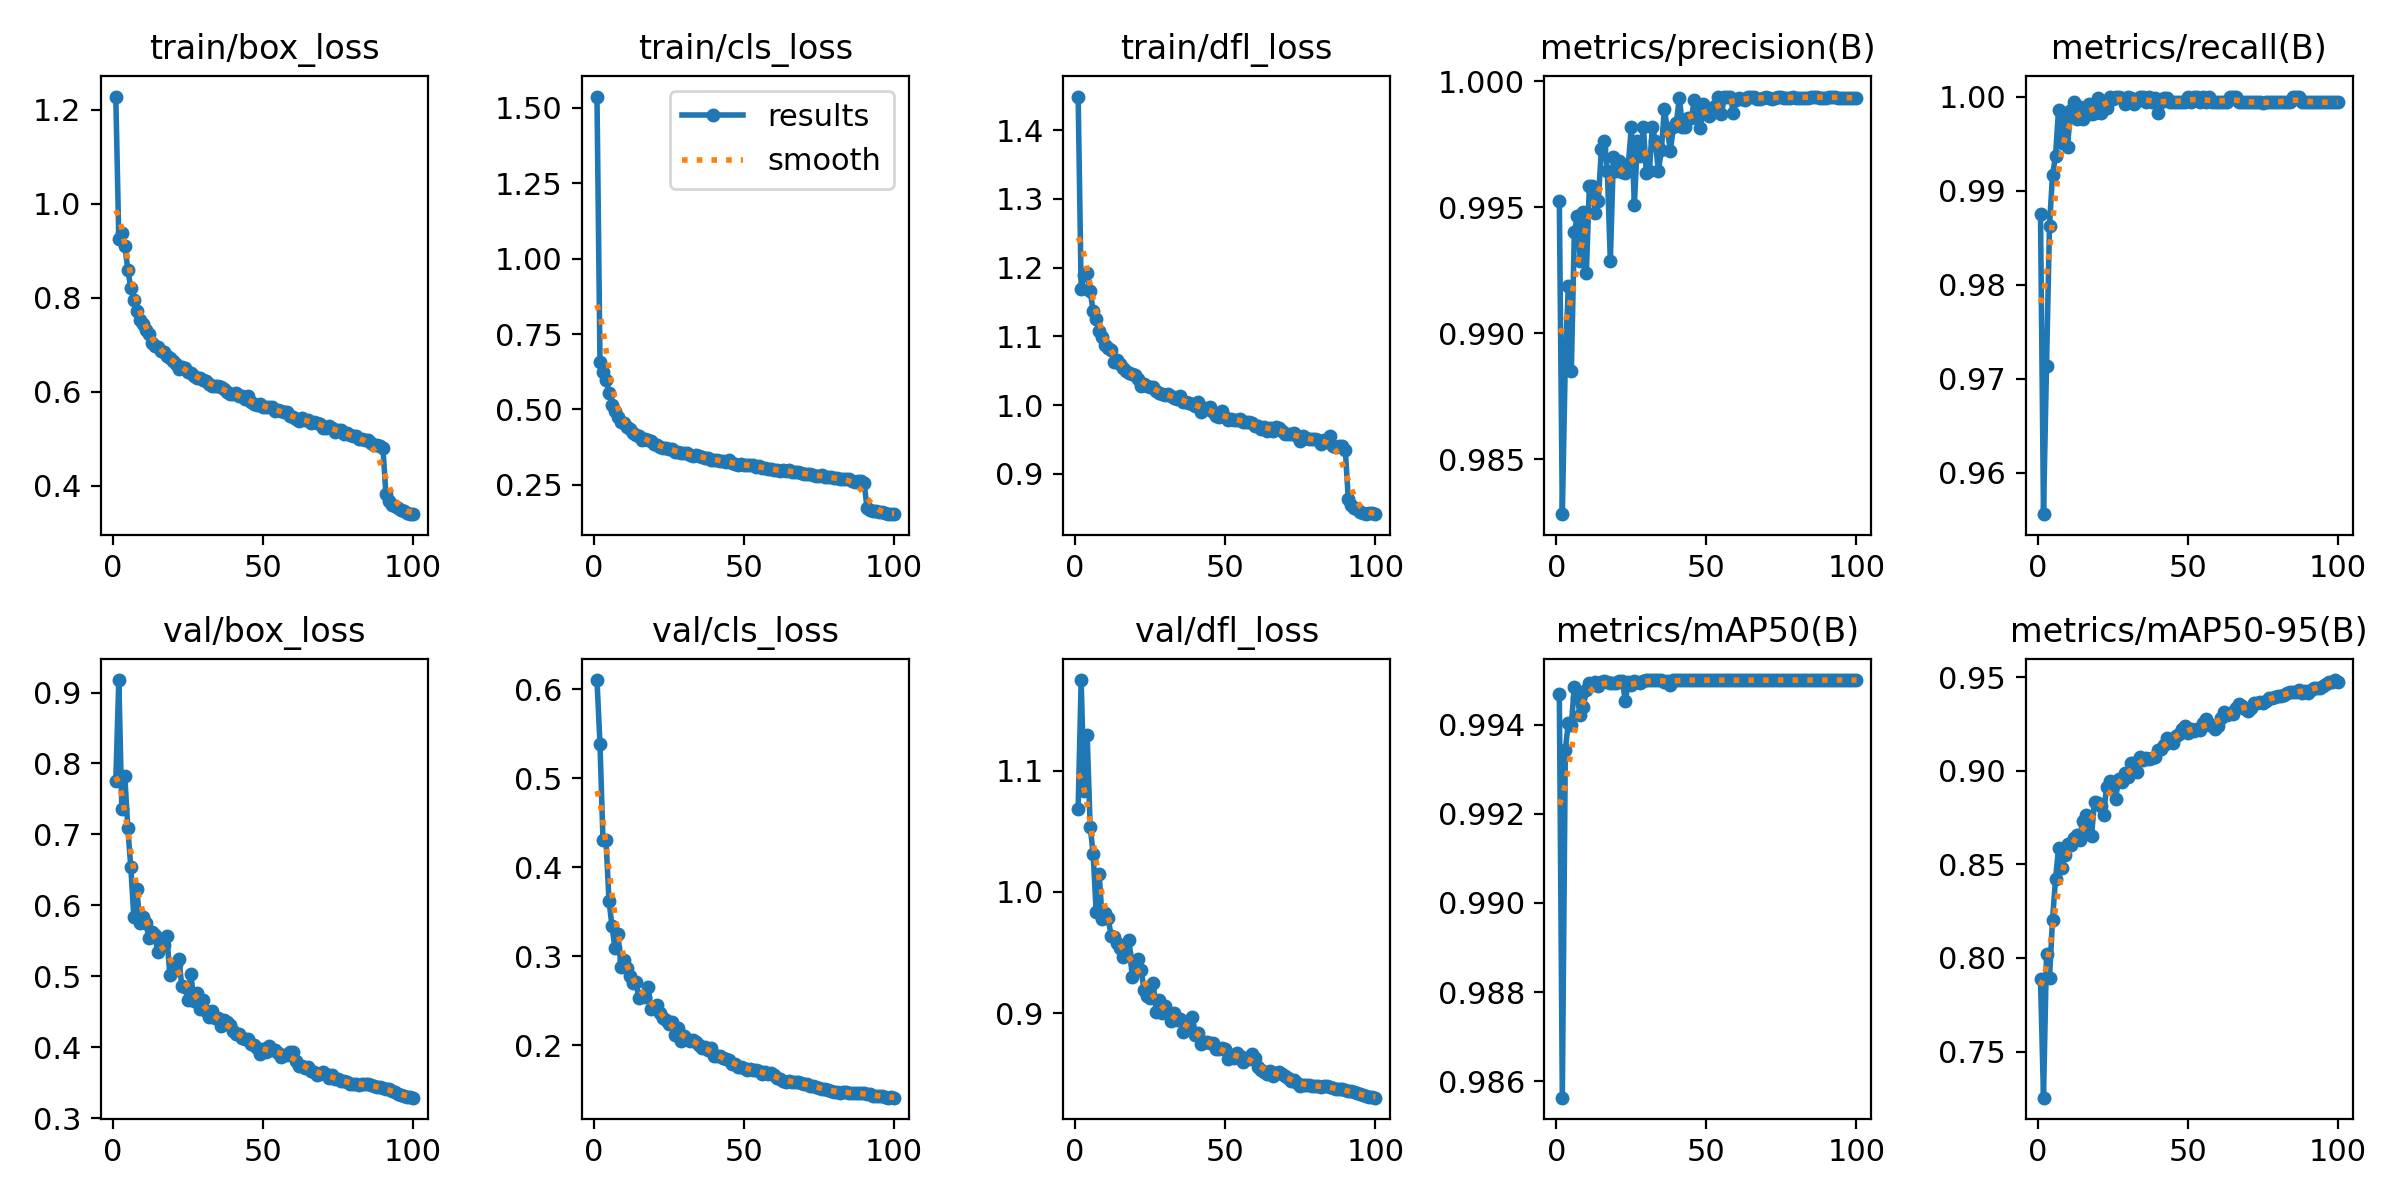
\includegraphics[width=0.8\textwidth]{images/results.png}
    \caption{Trainingsverlauf und Metriken des YOLO-Objektdetektors.}
    \label{fig:training_det}
\end{figure}

Die Wahrheitsmatrix (\emph{engl. Confusion Matrix}) der Objekterkennung (Abbildung \ref{fig:confusion_det}) verdeutlicht die Präzision bei der Lokalisierung. Sie zeigt, dass bei der Validierung 1.676 Katzengesichter korrekt erkannt wurden. Das Modell hat jedoch zwei Katzengesichter erkannt, obwohl dort keines war, und eines hat es komplett übersehen. Die Matrix belegt also dass der Detektor nahezu fehlerfrei auf den Validierungsdaten funktionierte.

\begin{figure}[H]
    \centering
    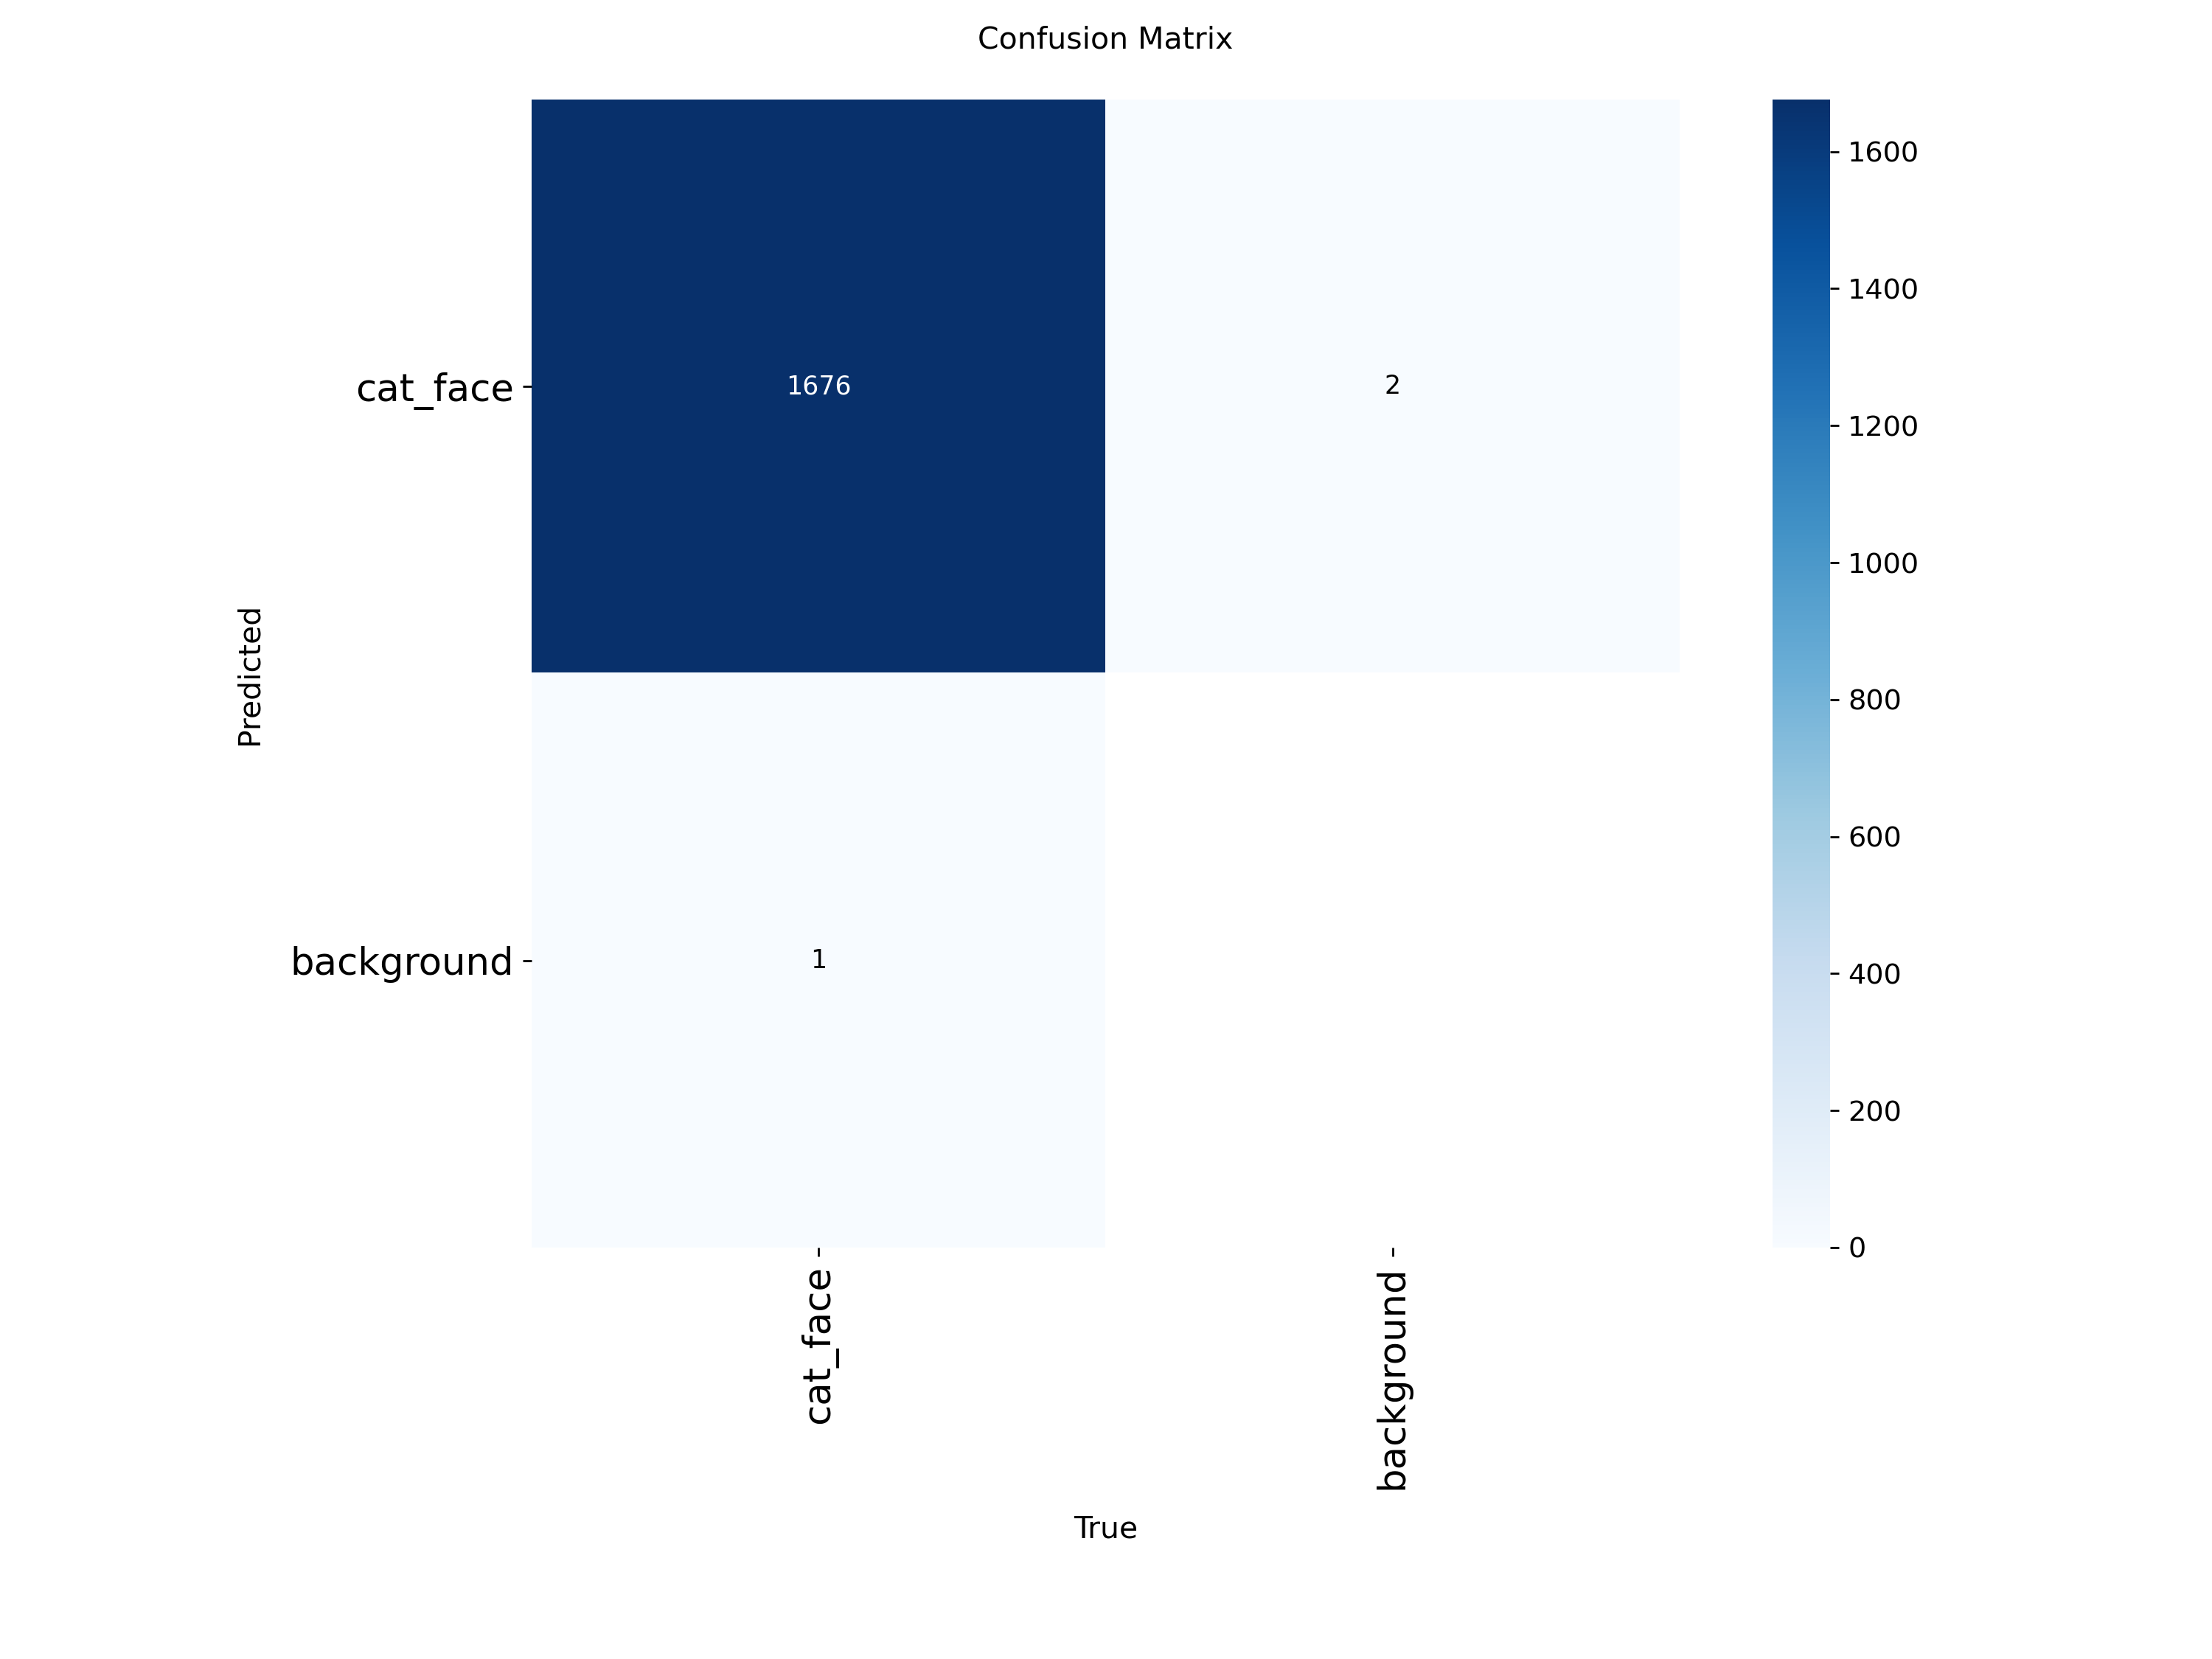
\includegraphics[width=0.6\textwidth]{images/confusion_matrix.png}
    \caption{Wahrheitsmatrix (Detektor).}
    \label{fig:confusion_det}
\end{figure}

Eine wichtige Metrik, welche auch auf den Validierungsdaten beruht, ist die Präzision-Trefferquote-Kurve (\emph{engl. Precision-Recall-Curve}), sie gibt das Verhältnis zwischen richtig erkannten Objekten und Fehlalarmen an wie sicher  das Modell ist \cite{everingham2010pascal, lin2014coco}. In diesem Fall zeigt der Verlauf, dass das Modell extrem sicher ist und nicht raten muss, wenn es ein Katzengesicht sieht.

\begin{figure}[H]
    \centering
    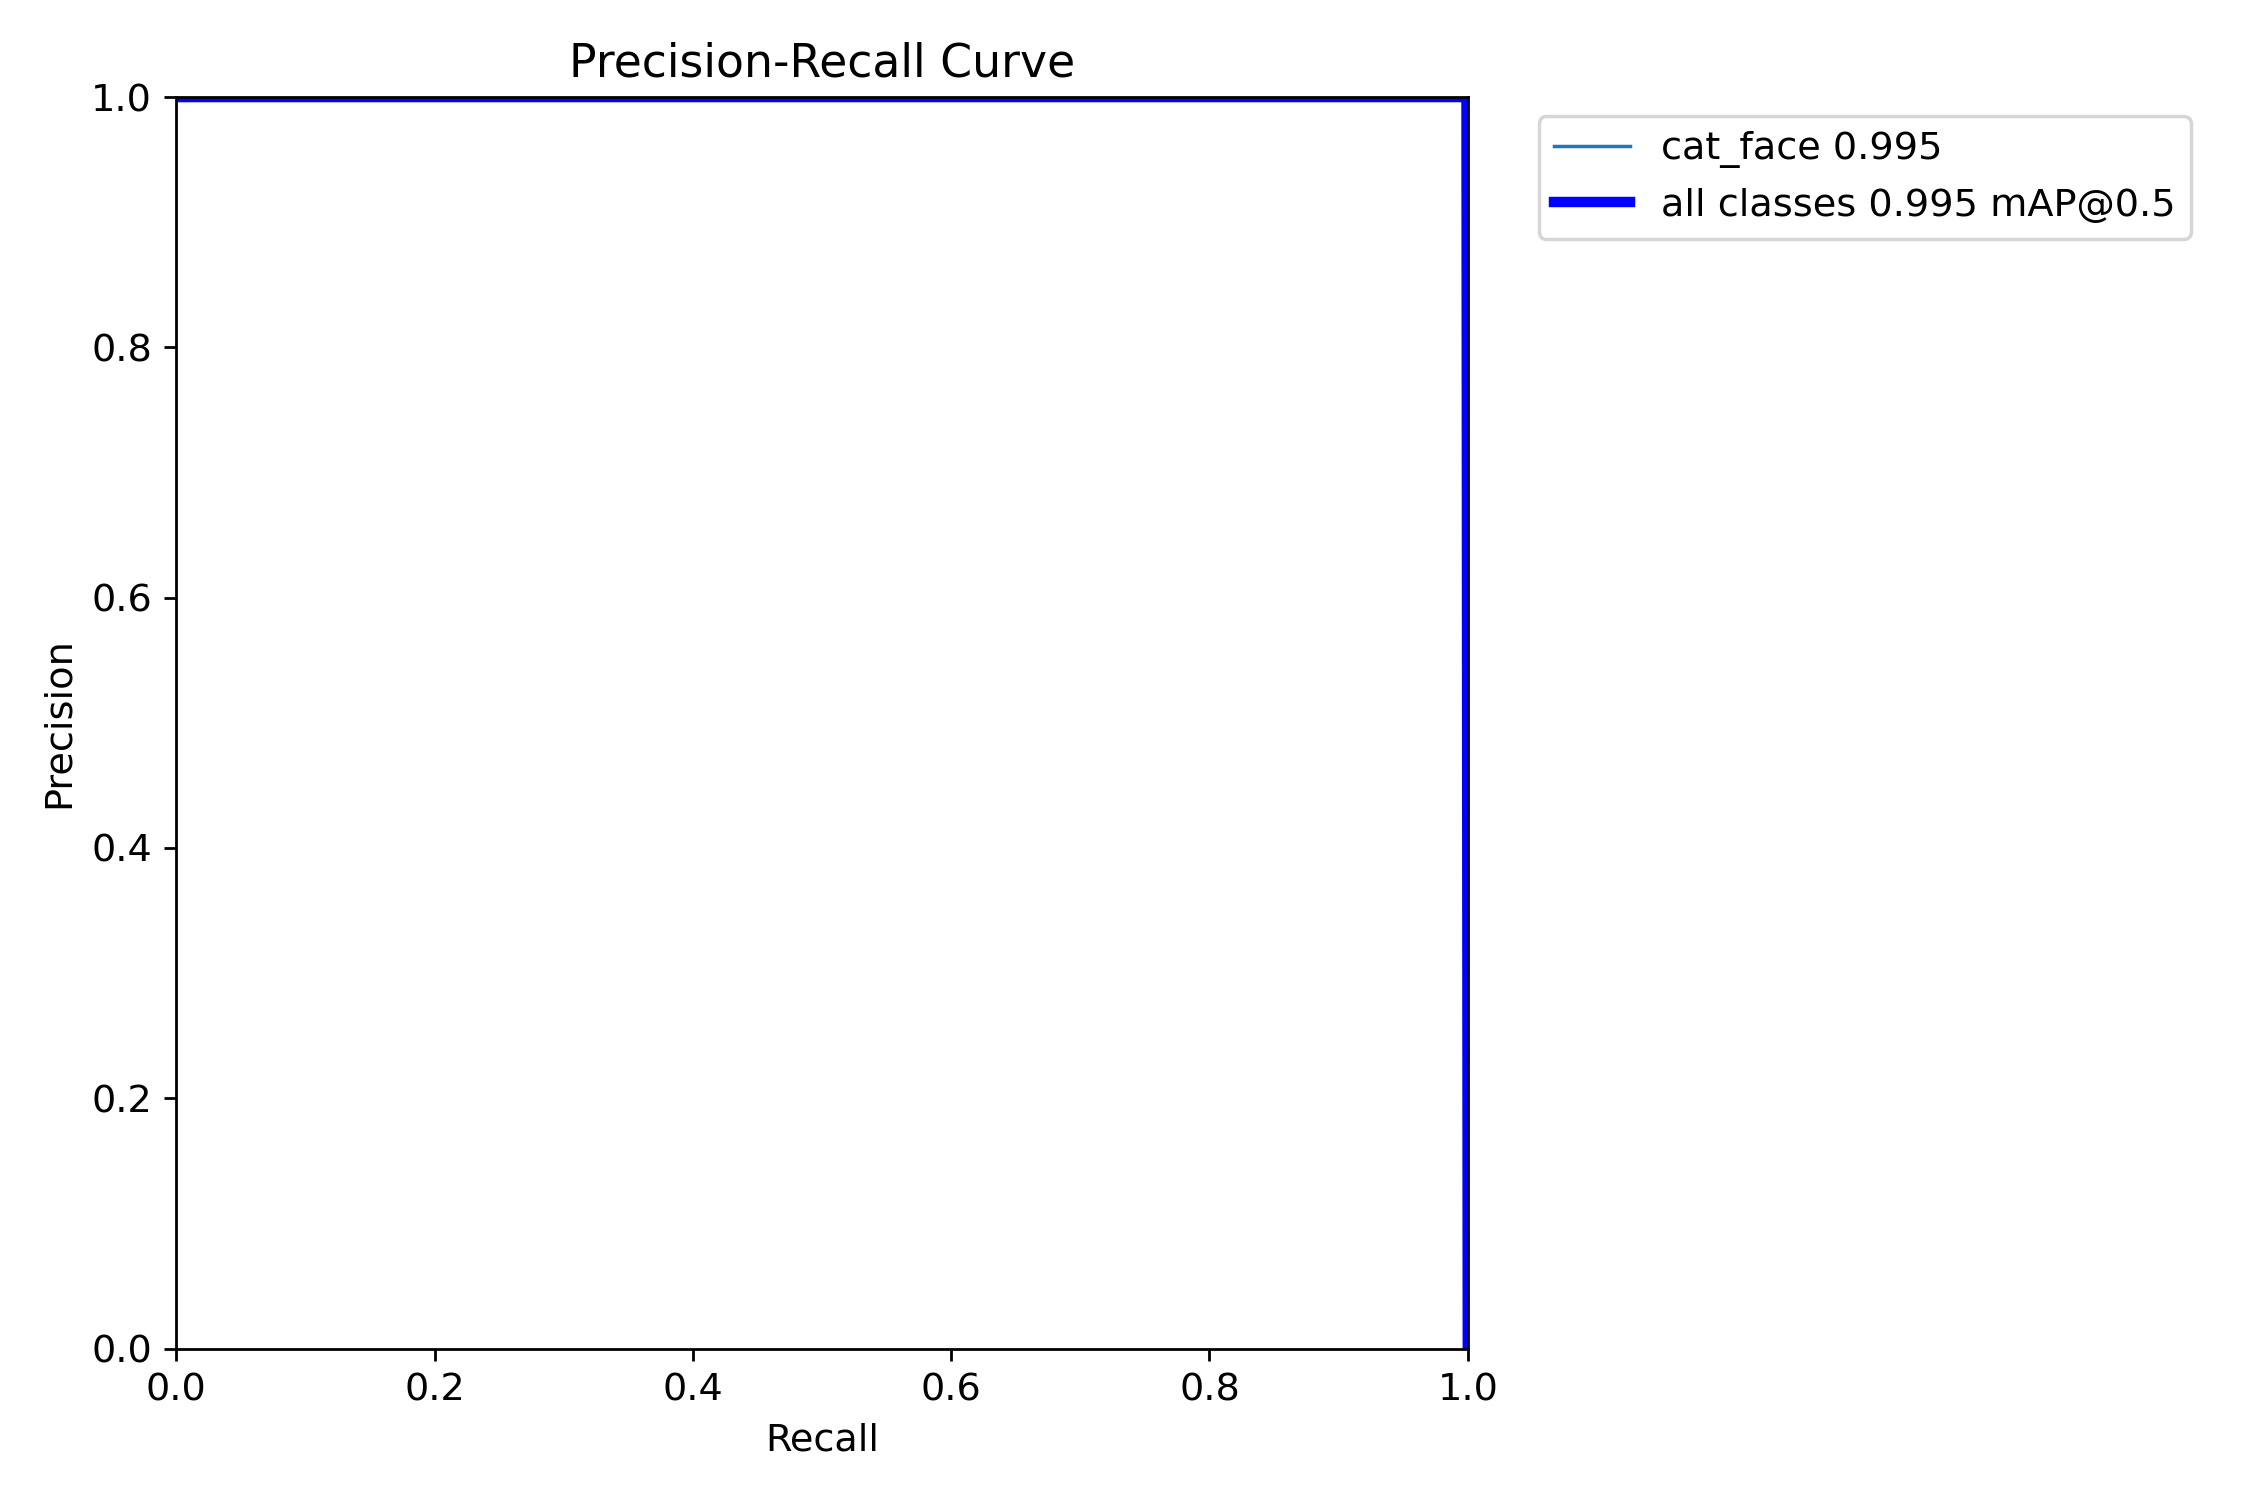
\includegraphics[width=0.6\textwidth]{images/BoxPR_curve.png}
    \caption{Präzision-Trefferquote-Kurve (\emph{engl. Precision-Recall-Curve}).}
    \label{fig:pr_curve_det}
\end{figure}

Die F1-Maß-Kurve (Abbildung \ref{fig:f1_curve_det}) zeigt wie sich die Leistung des Modells bei Änderung des Konfidenzschwellenwerts \cite{ultralytics_confidence} verändert. Dadurch können wir den optimalen Schwellenwert für den realen Betrieb des Modells ermitteln. Da die Kurve bis $\approx 0,85$ flach bleibt, d.h. hier wird keine Katze übersehen, fällt sie $> 0{,}85$ stark ab. Das zeigt, dass ab diesem Schwellenwert auch reale Katzen leicht übersehen werden. In der Praxis zeigt sich, dass bei einem Konfidenzschwellwert von $\approx 0,75$ ein gutes Verhältnis zwischen „Katze wird nicht erkannt“ und „es wird eine Katze erkannt, wo sich keine befindet“ entsteht. Im Betrieb wird der Detektor dennoch mit einem niedrigen Schwellenwert von 0,1 ausgeführt, da ByteTrack auch Erkennungen mit niedrigem Konfidenzwert für die Zuordnung verwendet \cite{zhang2022bytetrack}.

\begin{figure}[H]
    \centering
    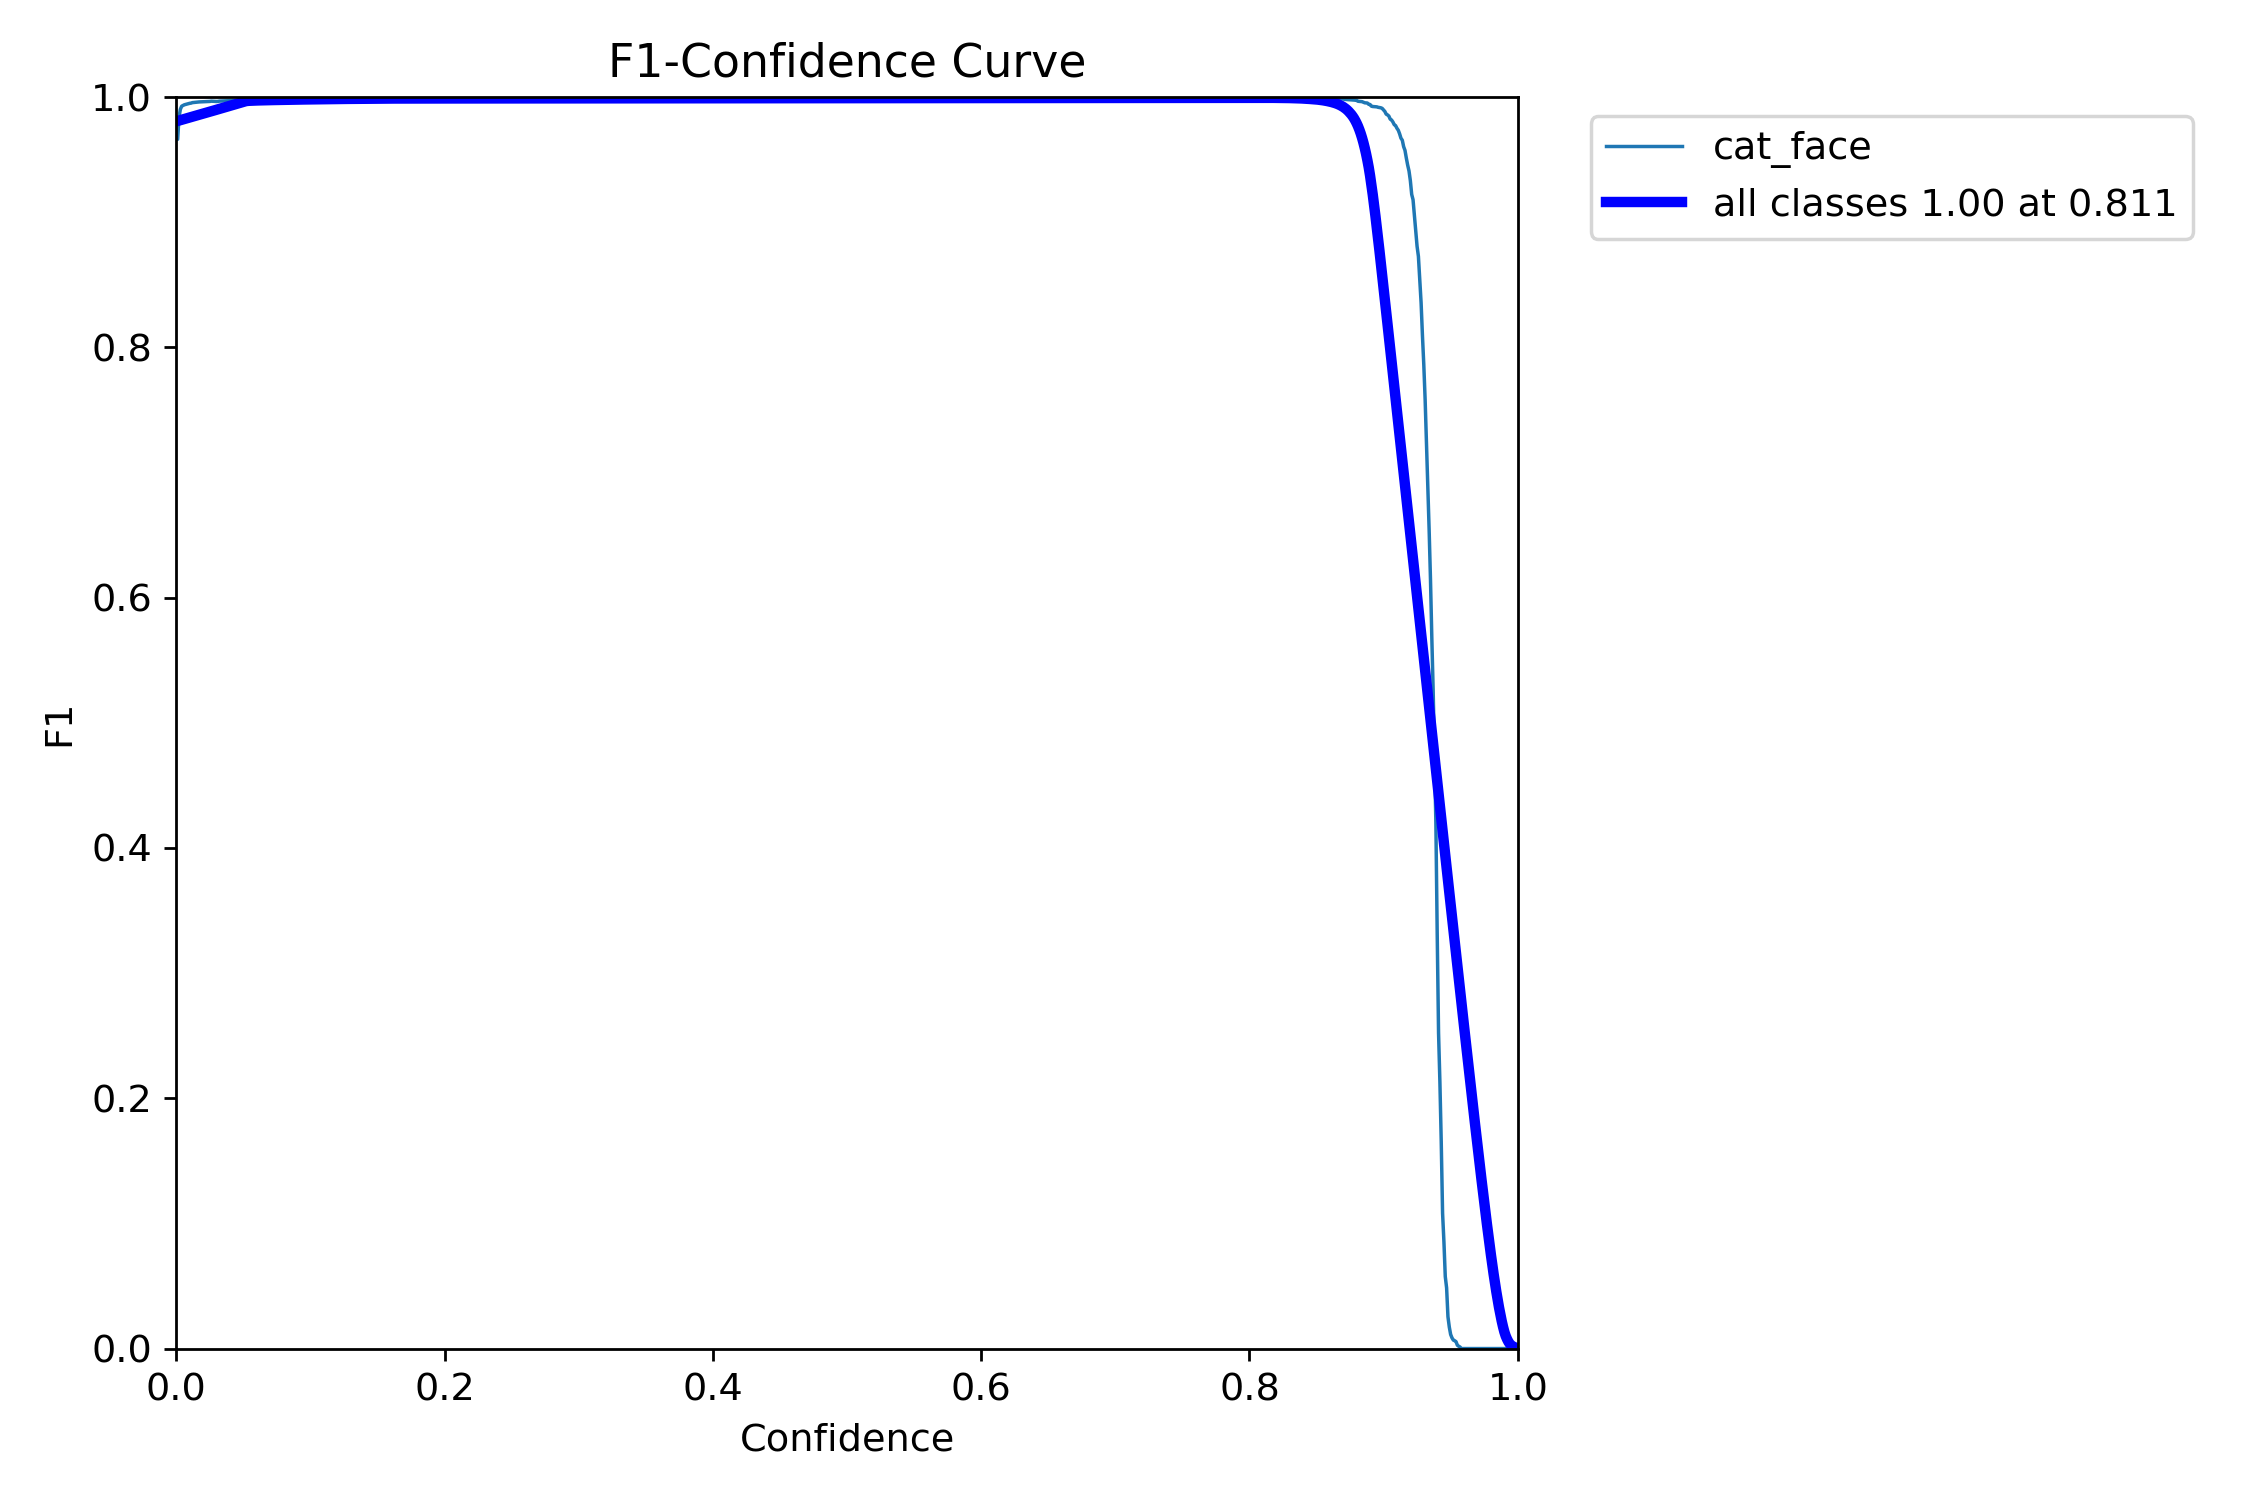
\includegraphics[width=0.6\textwidth]{images/BoxF1_curve.png}
    \caption{F1-Maß-Kurve.}
    \label{fig:f1_curve_det}
\end{figure}

Die Abbildung \ref{fig:val_pred_det} liefert einen Eindruck auf die Erkennungsleistung des Modells, wenn man es auf die Validierungsdaten ansetzt.

\begin{figure}[H]
    \centering
    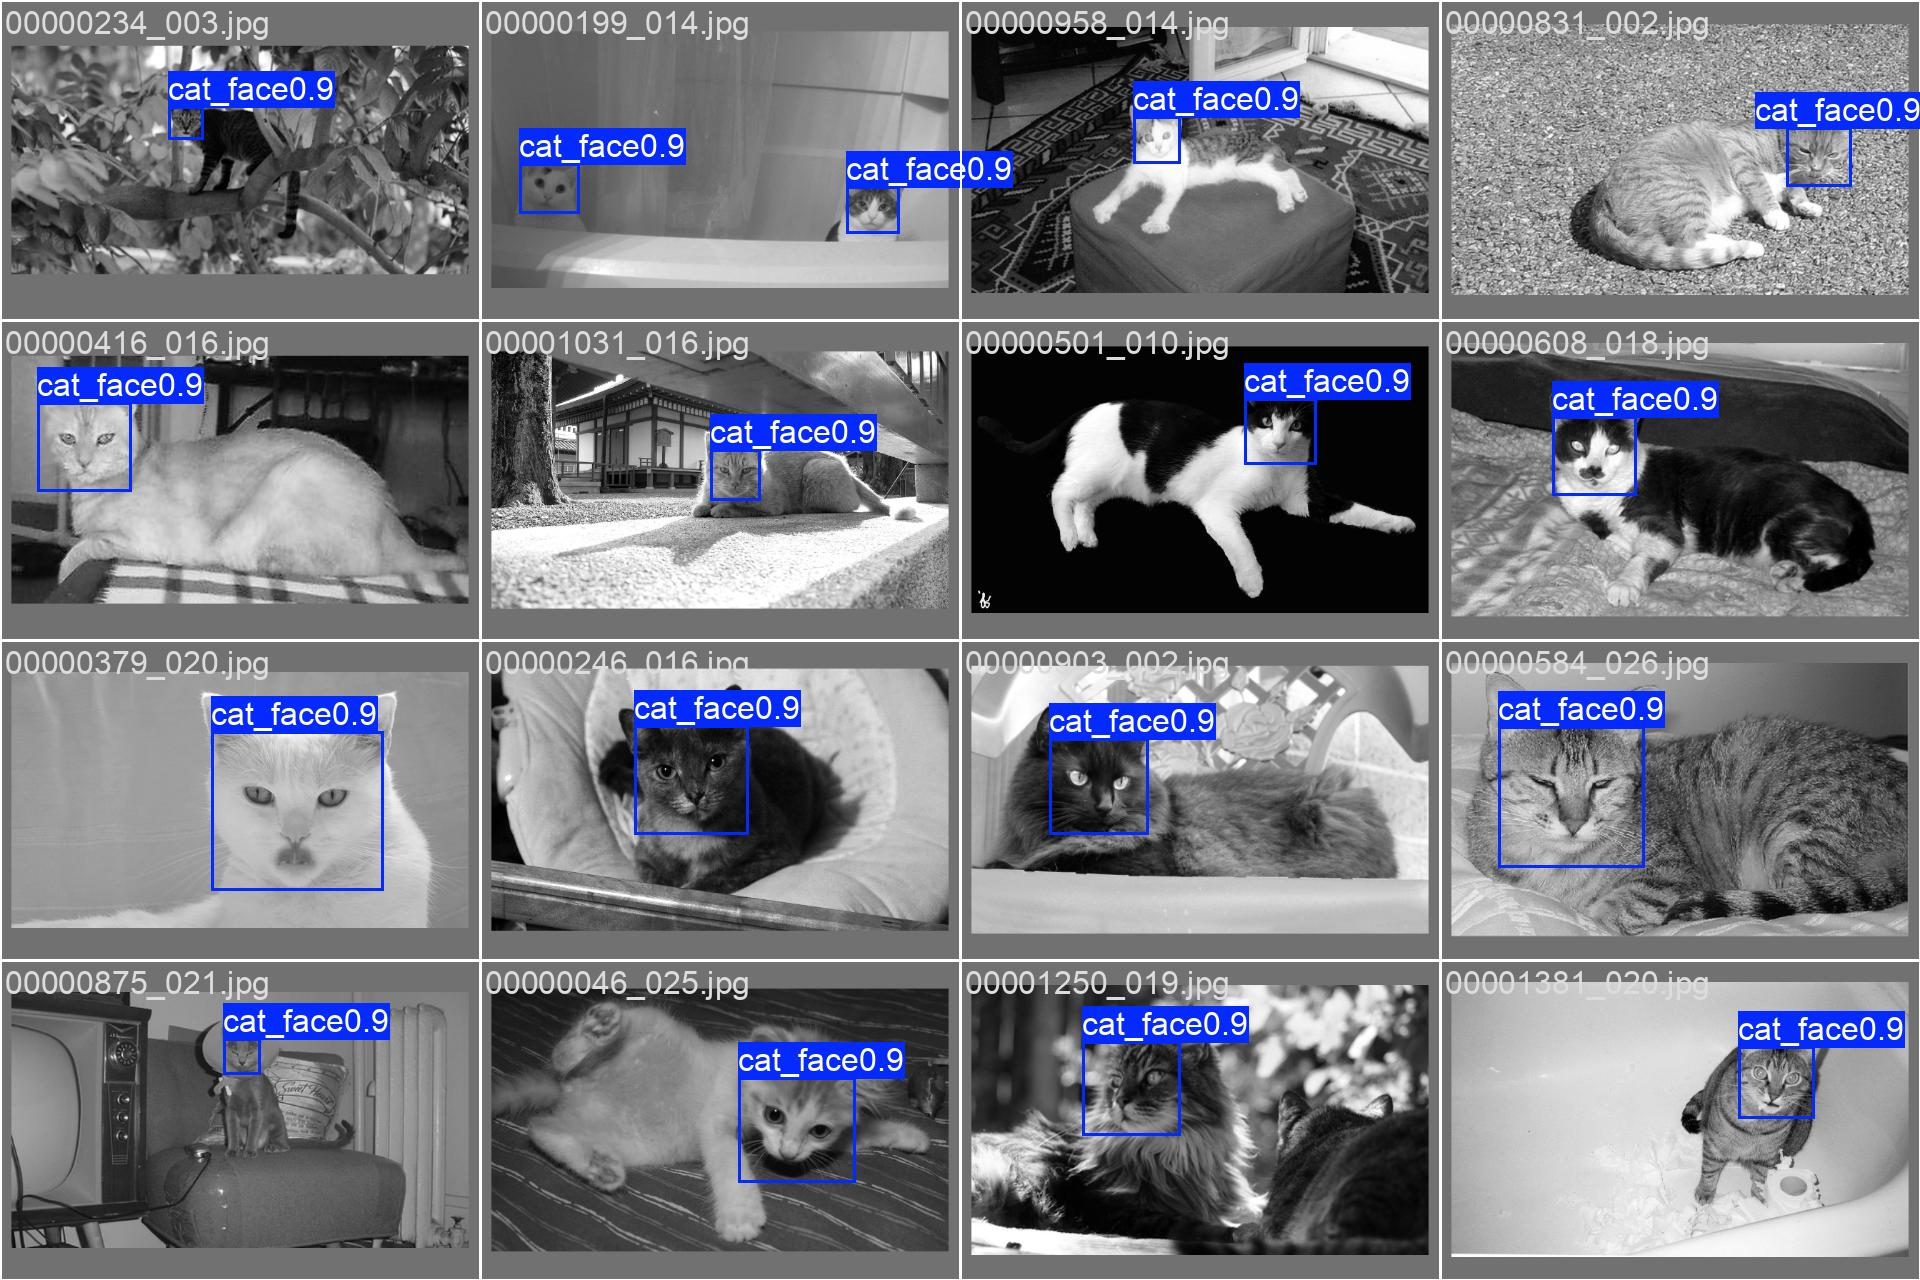
\includegraphics[width=0.8\textwidth]{images/val_batch0_pred.jpg}
    \caption{Vorhersagen des Detektors auf dem Validierungsdatensatz.}
    \label{fig:val_pred_det}
\end{figure}

\subsection{Leistung der Bildsegmentierung}
Die folgenden Trainingsmetriken des Beute-Segmentierungsmodells zeigen, dass das Modell seine Aufgabe erfolgreich gelernt hat.
Beim betrachten der Verlustfunktionen wird ersichtlich, dass das Modell über die Epochen weniger Fehler sowohl bei Training als auch Validierung macht, daraus können wir schließen, dass das Segmentierungsmodell lernt ohne sich dabei zu viel auf den Trainingsdatensatz anpasst.

\begin{figure}[H]
    \centering
    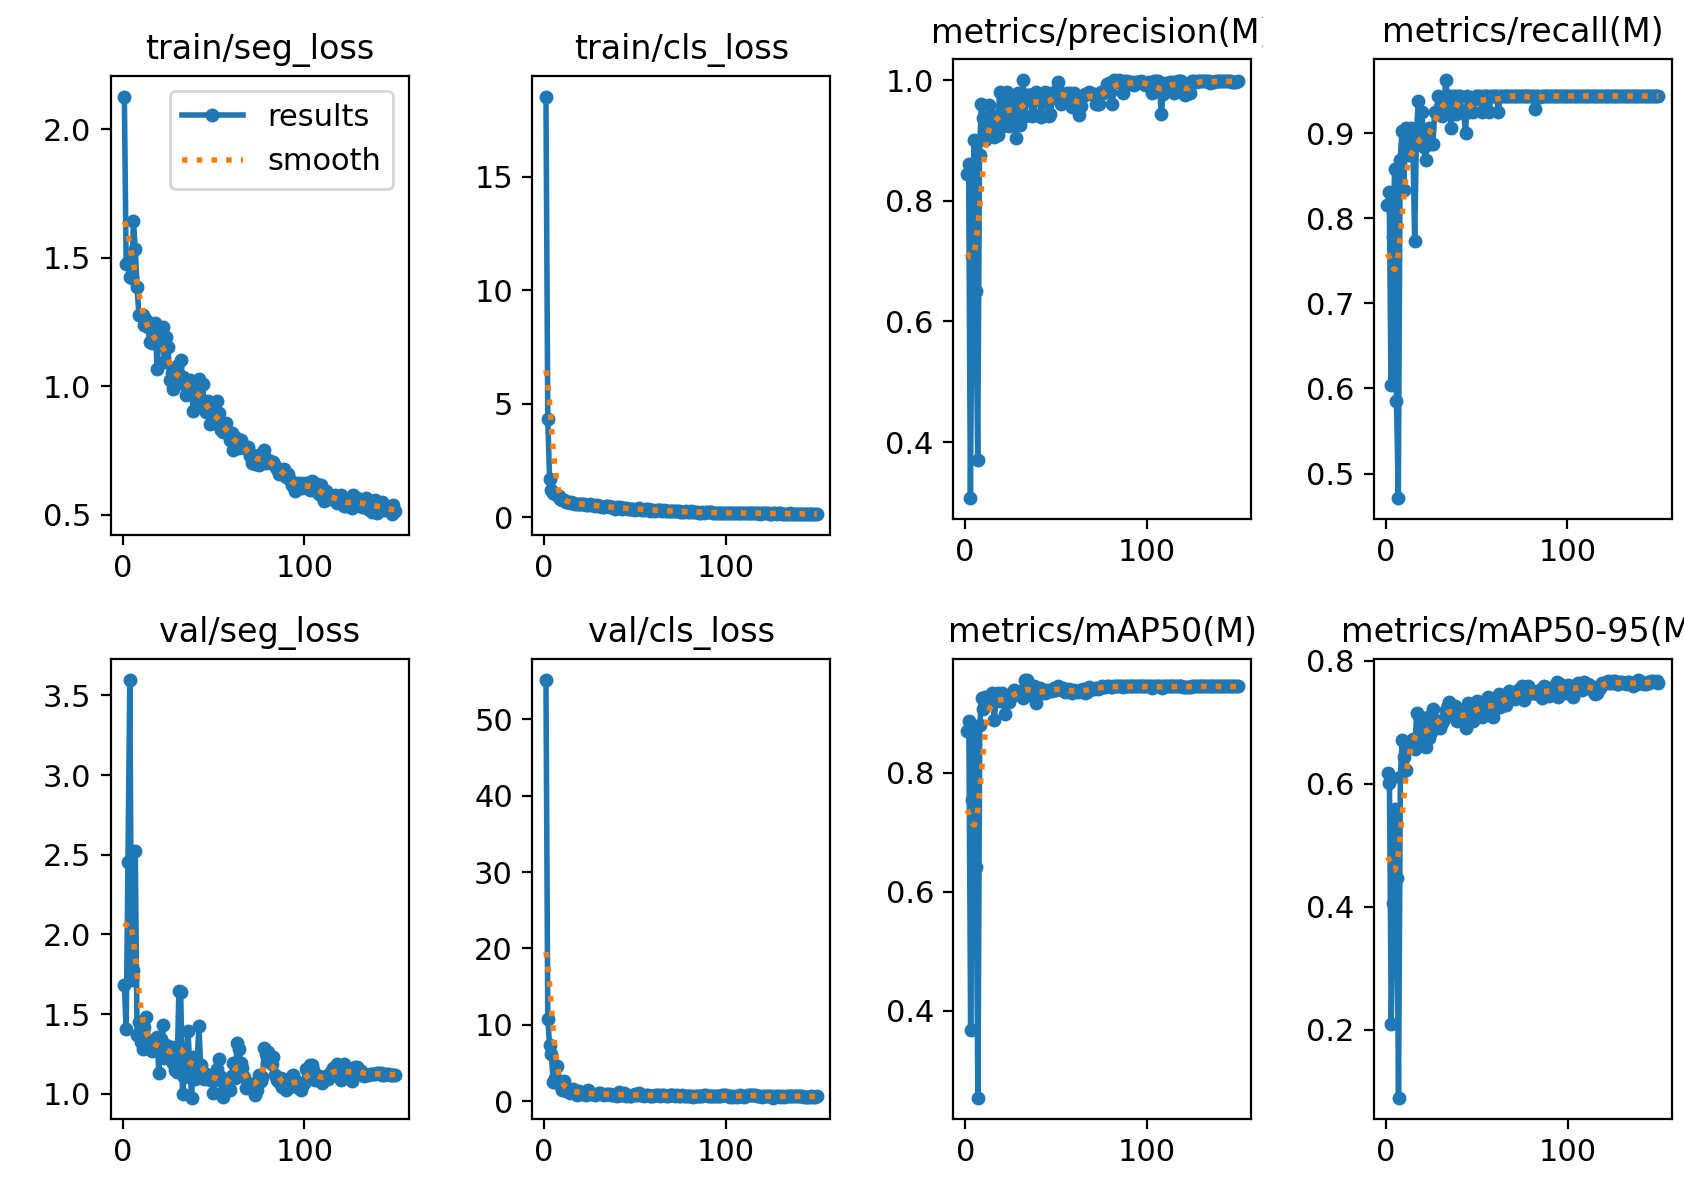
\includegraphics[width=0.8\textwidth]{images/seg_results.png}
    \caption{Trainingsverlauf und Metriken des YOLO-Segmentierungsmodells.}
    \label{fig:training_cls}
\end{figure}

Die Präzision-Trefferquote-Kurve der Segmentierungsmasken (Abbildung \ref{fig:pr_curve_seg}) zeigt, dass das Modell bis zu einer Trefferquote von etwa 94\,\% keine einzige Fehlerkennung liefert. Auf dem Validierungsdatensatz erreicht es eine mAP50 von 0,945.

\begin{figure}[H]
    \centering
    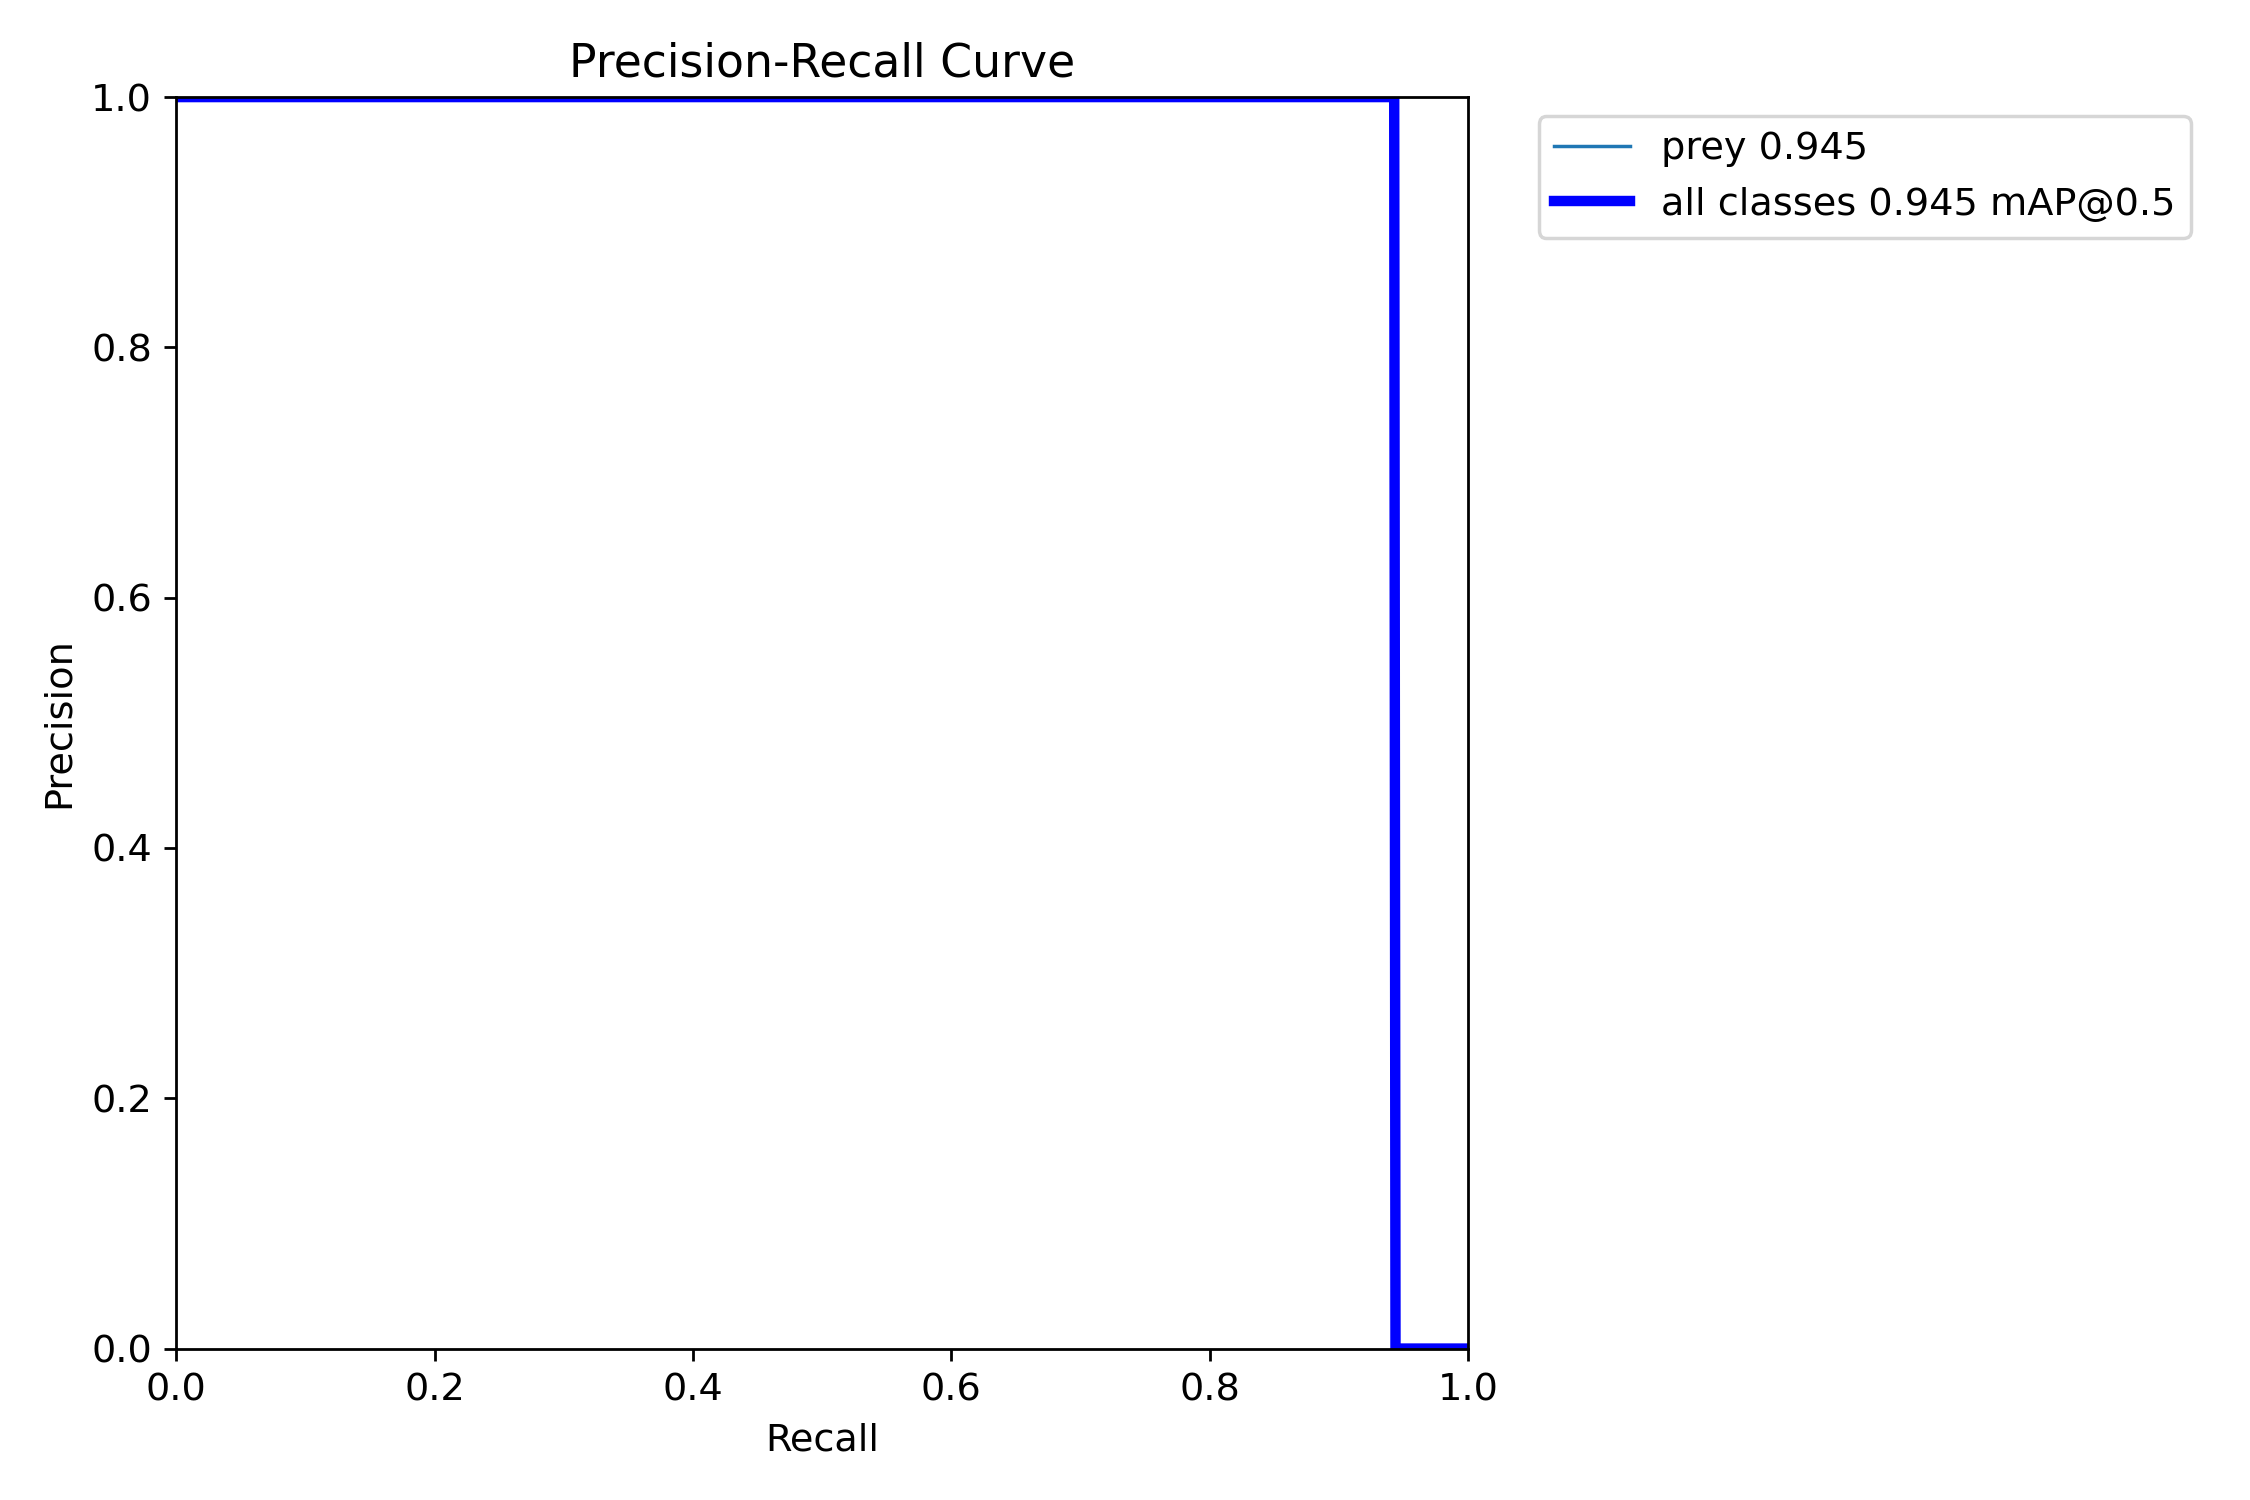
\includegraphics[width=0.6\textwidth]{images/seg_pr_curve.png}
    \caption{Präzision-Trefferquote-Kurve der Segmentierungsmasken.}
    \label{fig:pr_curve_seg}
\end{figure}

Die F1-Maß-Kurve (Abbildung \ref{fig:f1_curve_seg}) erreicht ihr Maximum von 0,97 bei einem Konfidenzschwellenwert von 0,728. Zwischen etwa 0,1 und 0,85 bleibt sie nahezu konstant, das Modell reagiert in diesem Bereich also kaum empfindlich auf die Wahl des Schwellenwerts.

\begin{figure}[H]
    \centering
    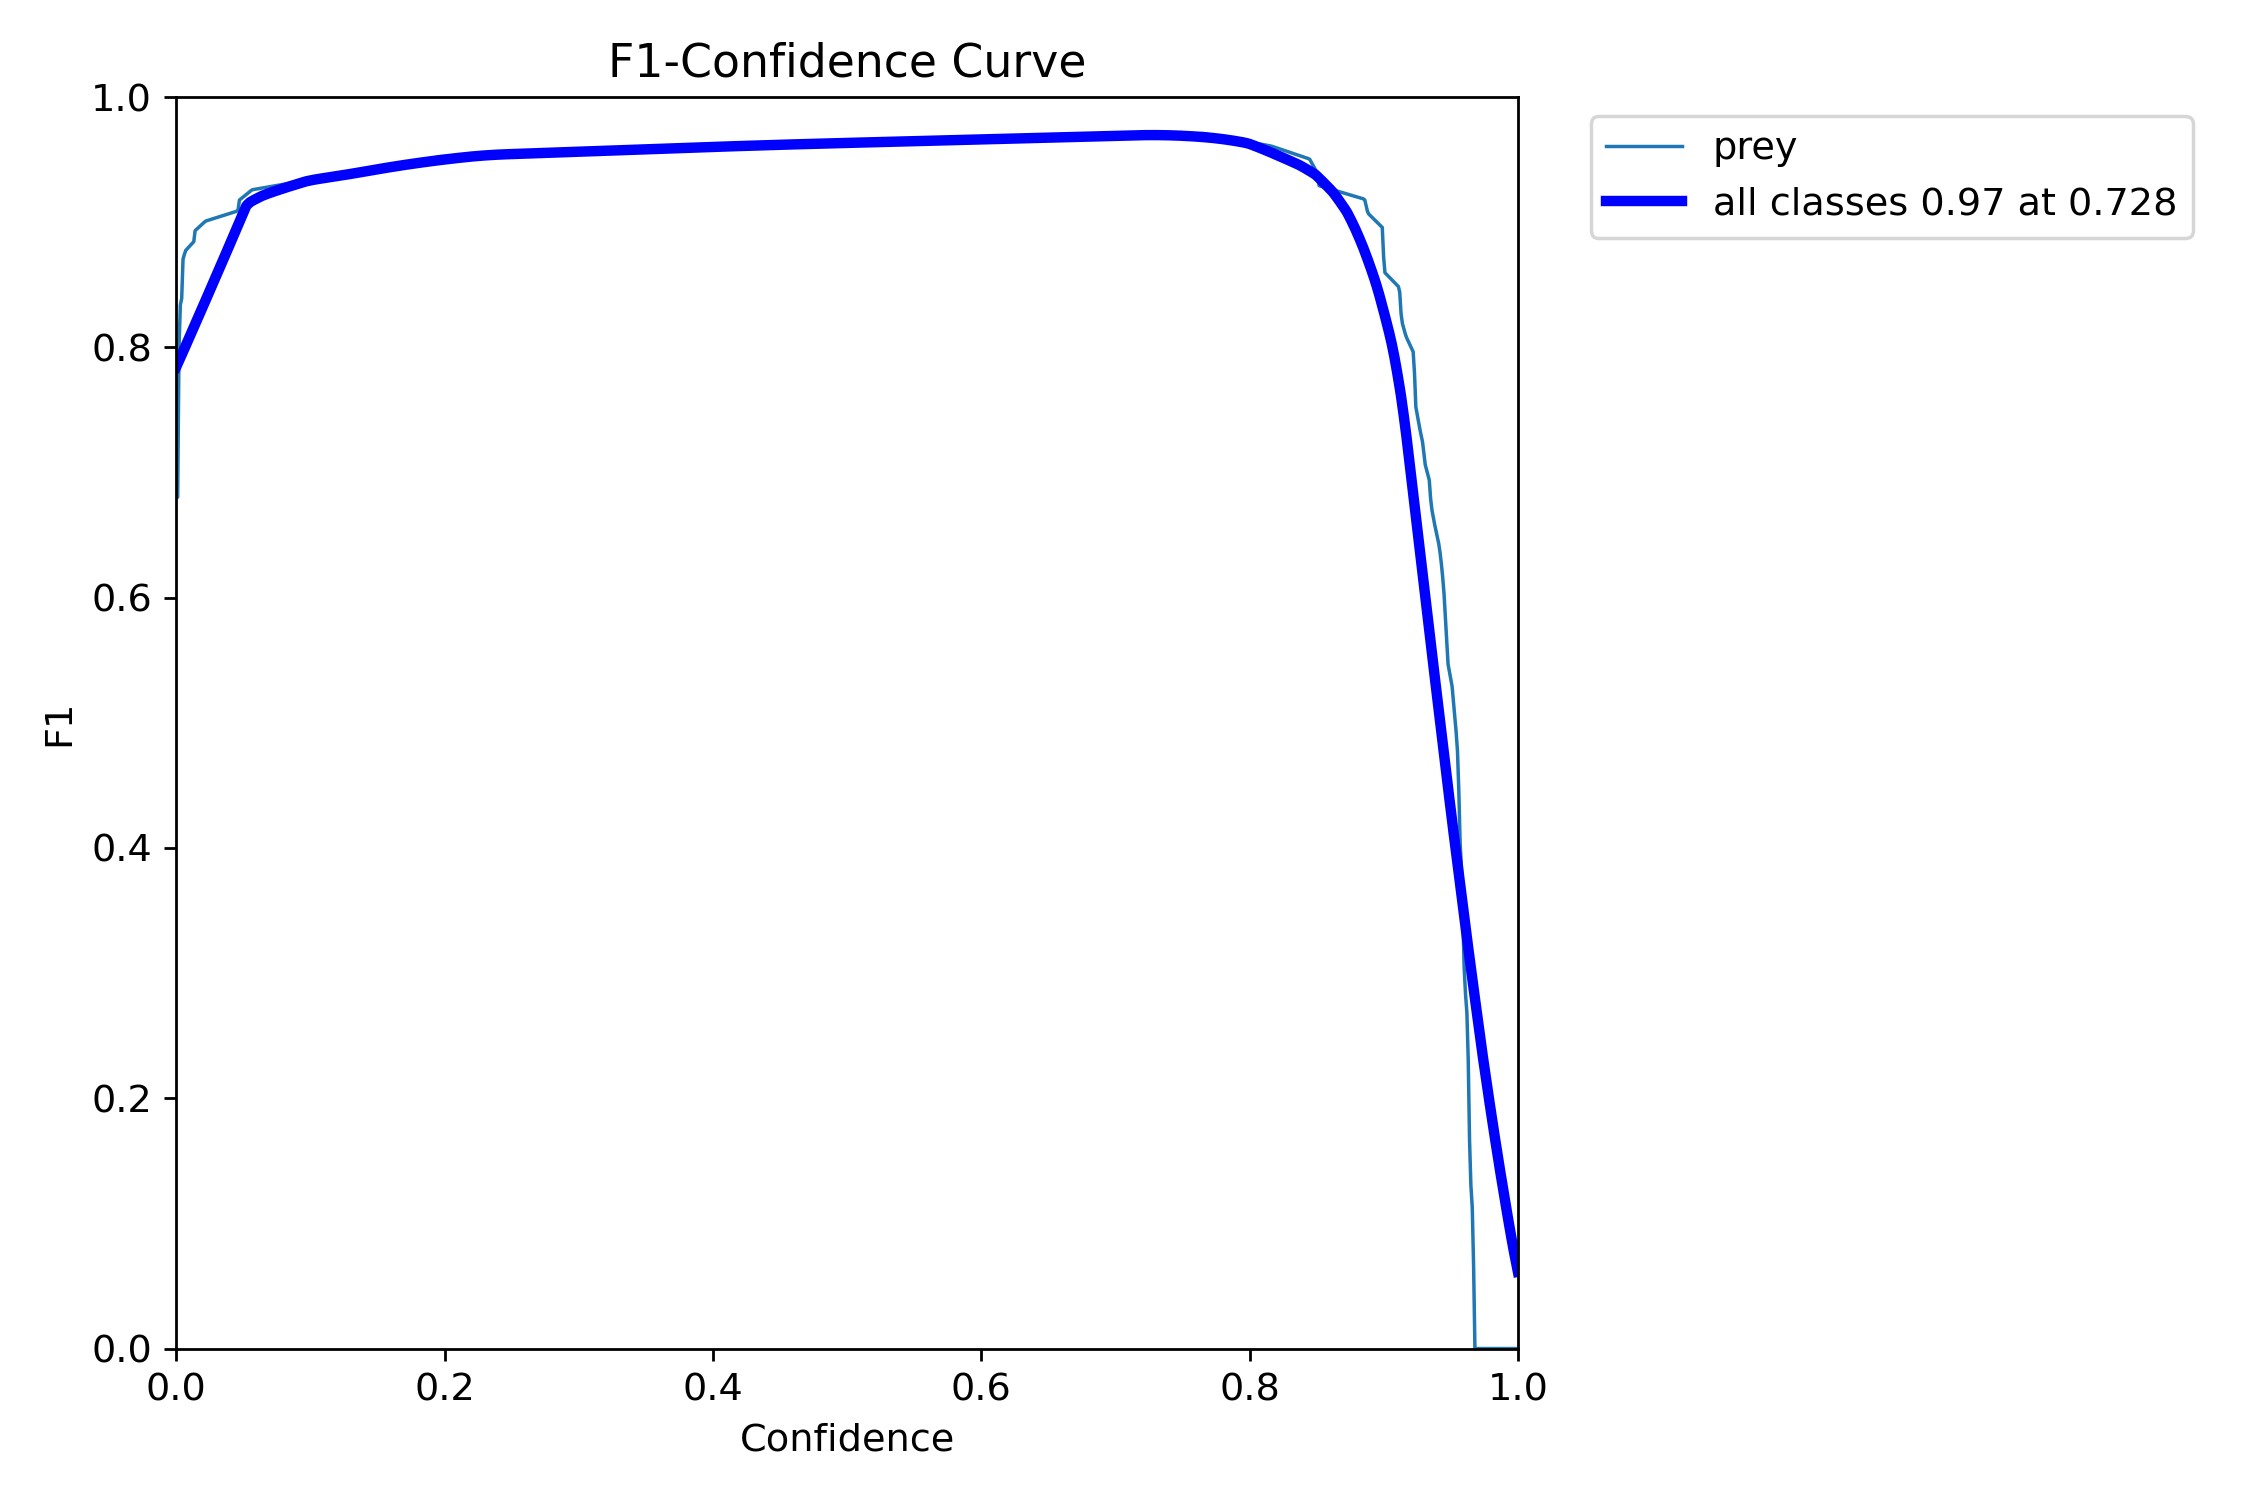
\includegraphics[width=0.6\textwidth]{images/seg_f1_curve.png}
    \caption{F1-Maß-Kurve des Segmentierungsmodells.}
    \label{fig:f1_curve_seg}
\end{figure}

Mithilfe der Abbildung \ref{fig:val_pred_cls} lässt sich gut erkennen, wie gut das Modell mit unbekannten Daten umgeht.

\begin{figure}[H]
    \centering
    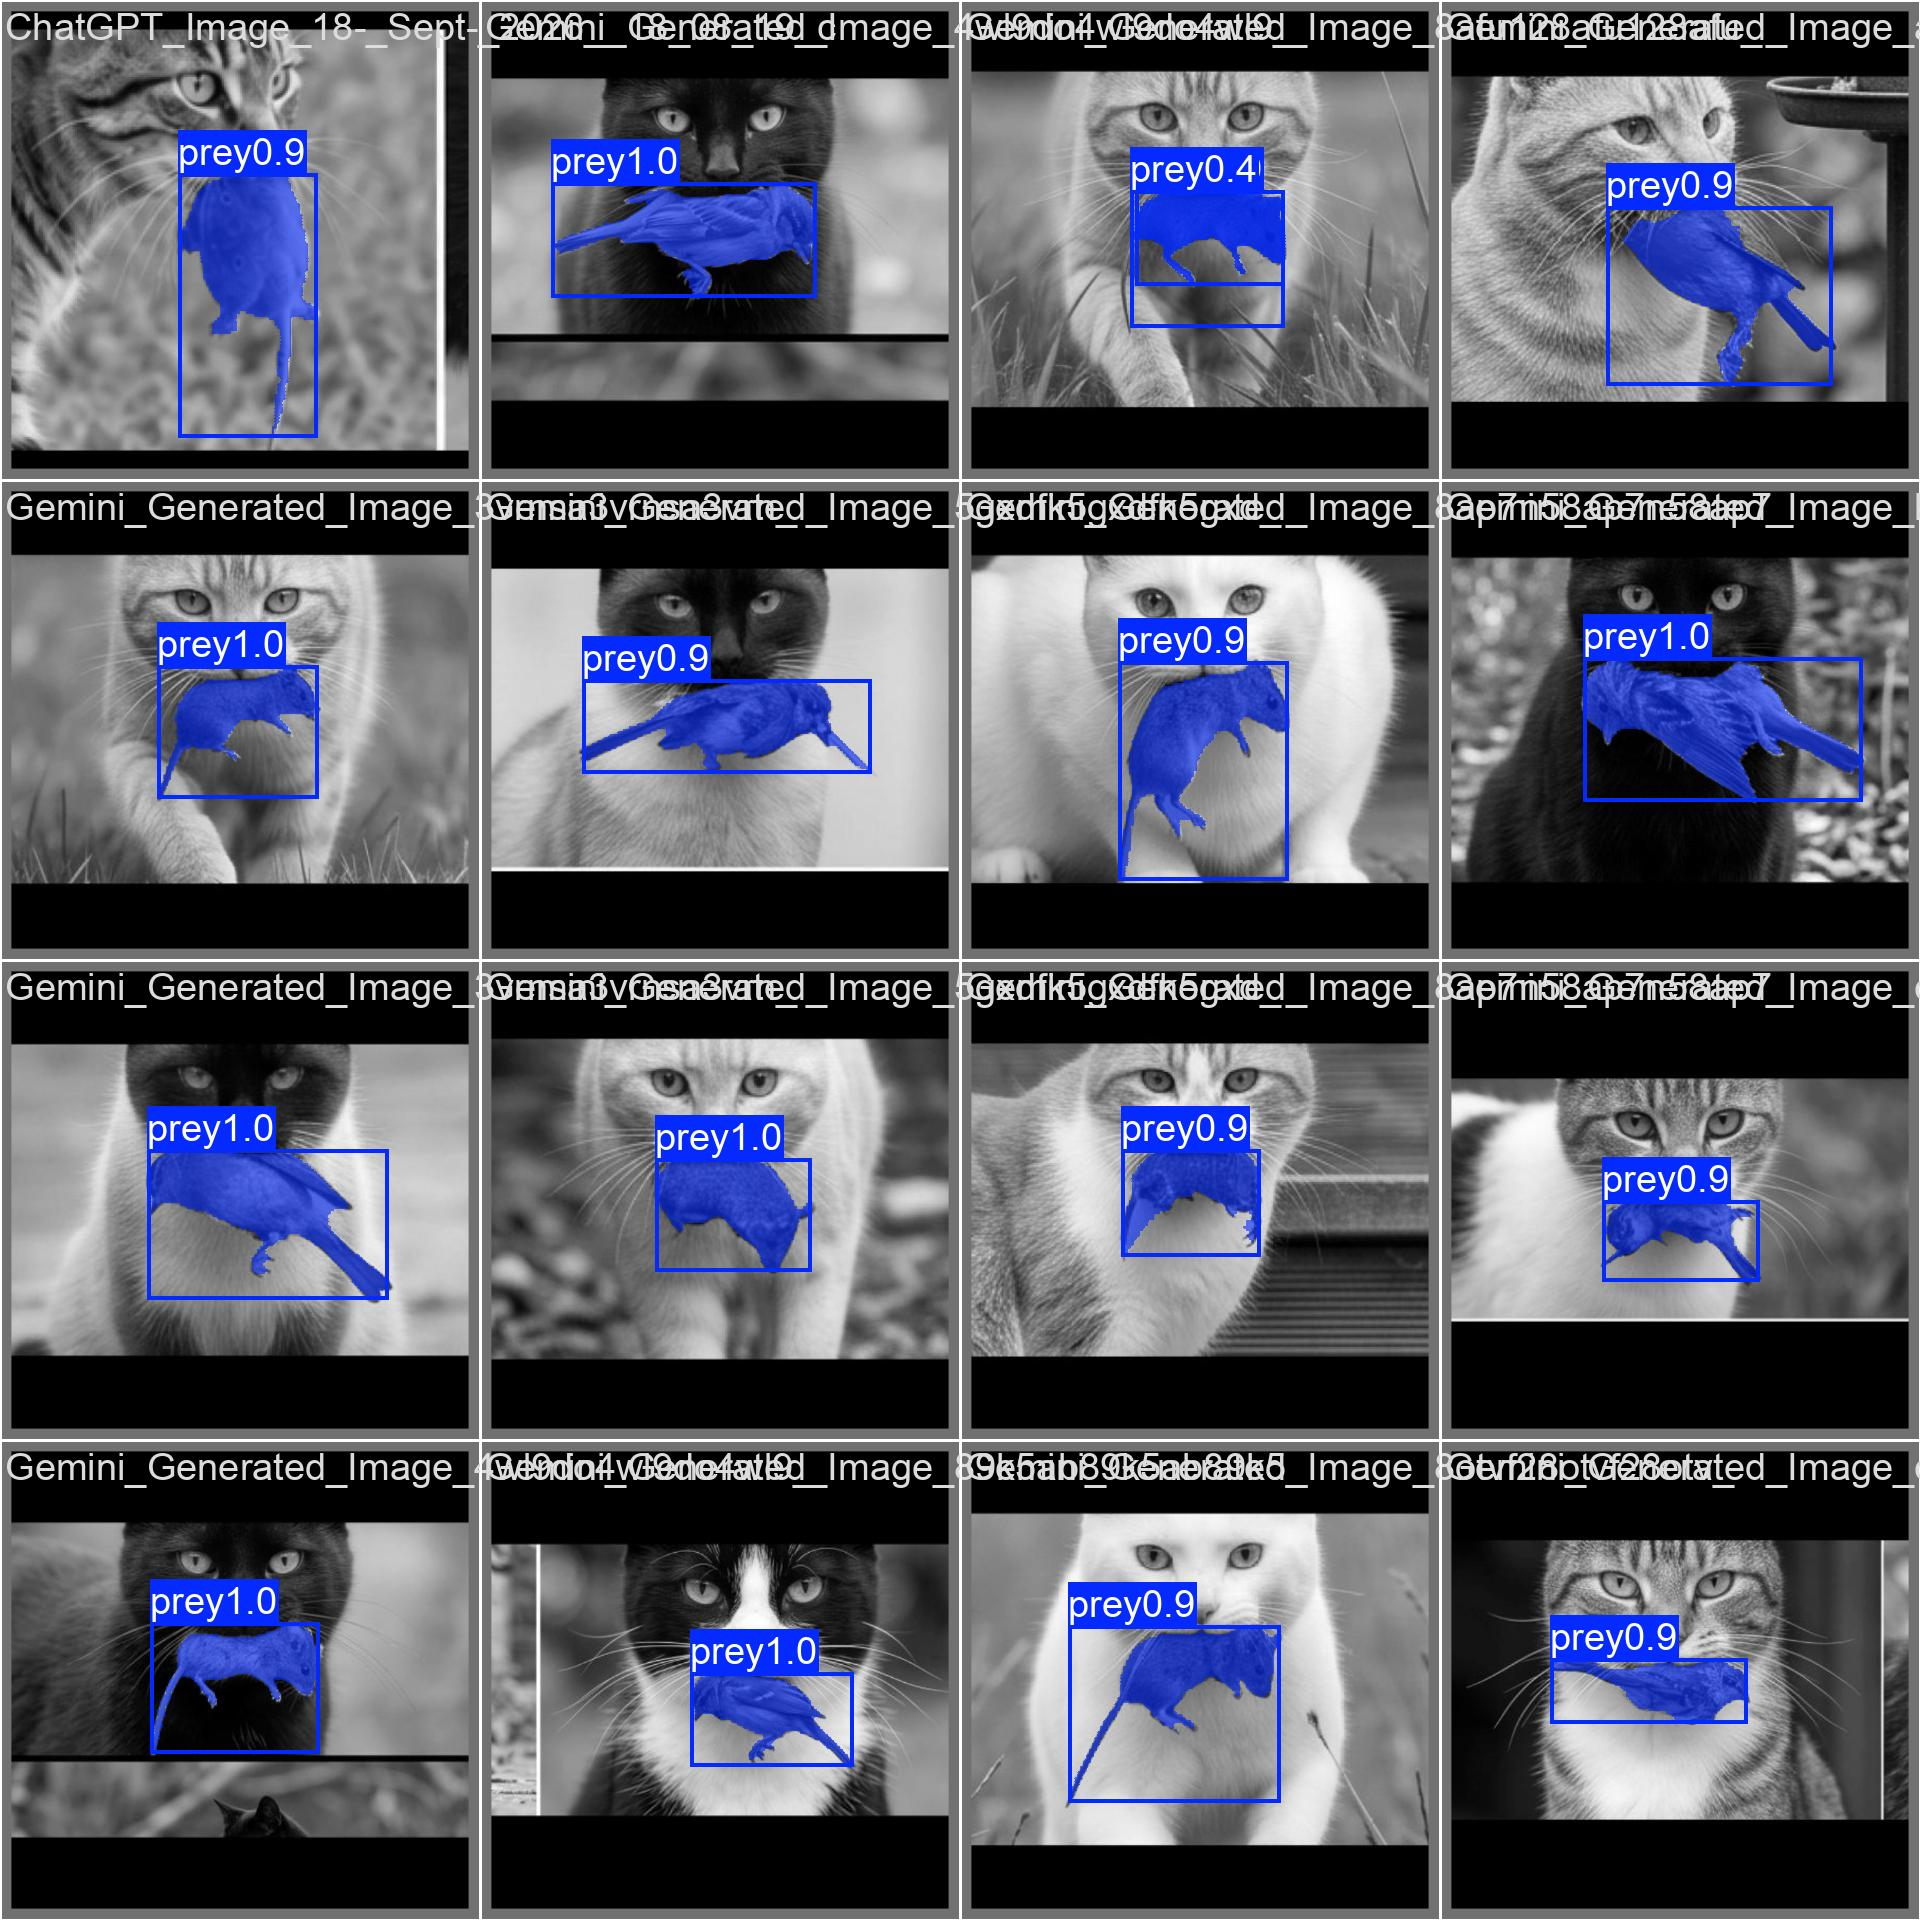
\includegraphics[width=0.8\textwidth]{images/seg_val_pred.jpg}
    \caption{Beispielhafte Vorhersagen des Segmentierungsmodells auf dem Validierungsdatensatz.}
    \label{fig:val_pred_cls}
\end{figure}

Rein auf dem Papier würden diese Modelle fast fehlerfreie Aussagen treffen. Die entscheidende Frage ist jedoch, wie verhält sich das System im Praxiseinsatz und welche Vorteile bietet die Verarbeitungskette gegenüber der reinen Detektion und Segmentierung.

\section{Evaluationsmethodik und Datensatz}
\label{sec:evaluationsmethodik}
Für die Evaluation des Gesamtsystems wird ein eigener Testdatensatz aus KI-generierten Videosequenzen erstellt. Dieses Kapitel beschreibt den Aufbau des Datensatzes, die Annotation der Referenzdaten und die verwendeten Metriken.

\subsection{Testdatensatz}
Die Testbasis bilden zehn Videopaare, die mit dem Videomodell Veo über Gemini \cite{geminiteam2023gemini} erzeugt werden. Jedes Video zeigt die Perspektive einer fest montierten Kamera unmittelbar über der Katzenklappe, auf die sich eine oder zwei Katzen zubewegen. Ein Videopaar besteht aus einer Sequenz, in der eine Katze ein Beutetier im Maul trägt, und einem Gegenstück mit identischer Szene und möglichst identischem Bewegungsablauf, in dem keine Katze Beute trägt. Dadurch unterscheiden sich die beiden Videos eines Paares ausschließlich im Vorhandensein der Beute.

Die Videopaare decken unterschiedliche Fellfarben, Beutetiere (Maus, Vogel, Ratte und Wühlmaus), Lichtverhältnisse (Tag, Dämmerung und Infrarot-Nachtsicht) sowie Szenen mit zwei Katzen ab. Die Videos besitzen eine Länge von zehn Sekunden bei 24 Bildern pro Sekunde. Da das System auf dem Raspberry Pi 5 rund 8 Bilder pro Sekunde verarbeitet, werden die Videos für die Evaluation auf 8 Bilder pro Sekunde ausgedünnt. Dadurch entsprechen die gemessenen Entscheidungszeiten dem realen Betrieb.

\subsection{Annotation der Referenzdaten}
Für jedes Video wird eine Referenzannotation erstellt. Sie legt für jede Katze die Zeitintervalle fest, in denen die Katze im Bild sichtbar ist, in denen ihr Gesicht erkennbar ist und in denen sie Beute trägt. Aus diesen Intervallen ergibt sich für jedes Einzelbild der korrekte Zustand der Katzenklappe: Befindet sich mindestens eine Katze mit Beute im Bild, muss die Klappe gesperrt sein, andernfalls darf sie geöffnet werden.

\subsection{Definition der System-Metriken}
Nachdem alle Videosequenzen die Verarbeitungskette durchlaufen sind, kann man die Metriken für das gesamte System erstellen. Diese leiten sich aus Wahrheitsmatrix ab:

\begin{itemize}
    \item \textbf{Richtig-Positiv-Ergebnis (\emph{engl. True Positive}) (TP):} Katze mit Beute darf nicht ins Haus (korrekte Sperrung).
    \item \textbf{Falsch-Negativ-Ergebnis (\emph{engl. False Negative}) (FN):} Katze mit Beute darf ins Haus (Beute gelangt fälschlicherweise hinein).
    \item \textbf{Richtig-Negativ-Ergebnis (\emph{engl. True Negative}) (TN):} Katze ohne Beute darf ins Haus (korrekter Durchlass).
    \item \textbf{Falsch-Positiv-Ergebnis (\emph{engl. False Positive}) (FP):} Katze ohne Beute darf nicht ins Haus (Fehlalarm).
\end{itemize}

Im Kontext einer Katzenklappe besitzt die Katze aus Nutzersicht die höchste Priorität. Ein Falsch-Positiv-Ergebnis (Fehlalarm) bedeutet, dass das Haustier grundlos vor einer verschlossenen Tür steht. Um das Vertrauen des Tieres in die Klappe nicht zu zerstören, liegt der Fokus der Evaluierung primär auf der Vermeidung solcher Fehlalarme (hohe Präzision). Ein seltenes Falsch-Negativ-Ergebnis (\emph{engl. False Negative}) (eine Maus gelangt ins Haus) wird im Tausch für eine stressfreie Nutzung der Klappe durch die Katze bewusst in Kauf genommen.


Anders als eine Bewertung auf Videoebene erfasst die bildweise Auswertung auch kurzzeitige Fehlentscheidungen. Für jedes Einzelbild mit sichtbarer Katze wird der Zustand der Klappe mit der Referenzannotation verglichen. Daraus ergeben sich folgende Kennzahlen:

\begin{itemize}
    \item \emph{Sicherheitsfehler}: Anteil der Einzelbilder, in denen die Klappe geöffnet ist, obwohl eine Katze mit Beute sichtbar ist.
    \item \emph{Komfortfehler}: Anteil der Einzelbilder, in denen die Klappe gesperrt ist, obwohl nur saubere Katzen sichtbar sind. Gezählt wird erst nach einer Entscheidungszeit von drei Sekunden ab dem Erkennen des Katzengesichts, da der Zustandsautomat zu Beginn bewusst sperrt.
    \item \emph{Präzision}, \emph{Trefferquote} und \emph{F1-Maß} der Entscheidung \glqq Klappe sperren\grqq\ über alle Einzelbilder mit sichtbarer Katze. Einzelbilder mit sauberen Katzen innerhalb der Entscheidungszeit werden dabei nicht berücksichtigt.
    \item \emph{Durchgelassene Beute}: Anzahl der Videos mit Beute, in denen die Klappe mindestens einmal geöffnet wurde.
    \item \emph{Entscheidungszeit}: Zeit vom Erkennen des Katzengesichts bis zur ersten korrekten Entscheidung, also bis zur Sperrung bei einer Katze mit Beute beziehungsweise bis zur Freigabe bei einer sauberen Katze.
    \item \emph{Übersehene Katzen}: Anteil der Einzelbilder mit erkennbarem Katzengesicht, in denen das System keine Katze detektiert.
\end{itemize}

Die Auswertung erfolgt in zwei Schritten. Zunächst werden Detektor und Segmentierungsmodell einmal pro Video und Konfiguration ausgeführt und die Ergebnisse jedes Einzelbildes protokolliert. Anschließend wird der Zustandsautomat auf diesen Protokollen nachgebildet. Dadurch lassen sich unterschiedliche Parameter des Zustandsautomaten ohne erneute Inferenz vergleichen.

\section{Ergebnisse der Evaluation}
Das Gesamtsystem wird in der finalen Konfiguration ausgewertet: Gesichtsdetektor und Segmentierungsmodell arbeiten auf Graustufenbildern, der Zustandsautomat verwendet ein Zeitfenster von 20 Einzelbildern und einen Schwellenwert von 0,3. Die Herleitung dieser Parameter ist in Abschnitt~\ref{sec:ablation_sm} beschrieben. Tabelle~\ref{tab:system_eval} fasst die Ergebnisse auf den 20 Videos des Testdatensatzes zusammen.

\begin{table}[H]
    \centering
    \begin{tabular}{lcc}
        \toprule
        Metrik & Videos mit Beute & Videos ohne Beute \\
        \midrule
        Sicherheitsfehler & 1,6\,\% & -- \\
        Komfortfehler & -- & 4,1\,\% \\
        Durchgelassene Beute & 3 von 10 & -- \\
        Ausgesperrte saubere Katzen & -- & 0 von 10 \\
        Entscheidungszeit & 0,13\,s & 0,67\,s \\
        \bottomrule
    \end{tabular}
    \caption{Ergebnisse des Gesamtsystems auf dem Testdatensatz.}
    \label{tab:system_eval}
\end{table}

Über alle Einzelbilder mit sichtbarer Katze erreicht die Entscheidung \glqq Klappe sperren\grqq\ eine Präzision von 0,980, eine Trefferquote von 0,984 und ein F1-Maß von 0,982. In 4,3\,\% der Einzelbilder mit erkennbarem Katzengesicht detektiert das System keine Katze. Getrennt nach Lichtverhältnissen liegt der Sicherheitsfehler bei Tagaufnahmen bei 1,9\,\% und bei Infrarot-Aufnahmen bei 1,2\,\%, der Komfortfehler bei 6,8\,\% beziehungsweise 0,0\,\%.

Keine saubere Katze wird dauerhaft ausgesperrt. In drei der zehn Videos mit Beute wird die Klappe kurzzeitig geöffnet. Die Analyse dieser Videos zeigt drei Ursachen:

\begin{itemize}
    \item Die Katze ist noch weit von der Kamera entfernt, wodurch die Beute im Bildausschnitt zu klein ist, um vom Segmentierungsmodell erkannt zu werden.
    \item Die Katze dreht den Kopf weg oder läuft am Ende des Videos unter der Kamera hindurch. Das Segmentierungsmodell liefert für diese Einzelbilder keine Beute, und nach Ablauf des Zeitfensters gilt die Katze als sauber.
    \item Der Tracker (ByteTrack) weist derselben Katze eine neue Identität zu. Der neue Track beginnt mit einer leeren Historie, wodurch die bisherigen Beuteerkennungen verloren gehen.
\end{itemize}

\section{Ablationsstudien}
In den folgenden Ablationsstudien wird jeweils eine Komponente des Systems entfernt oder ersetzt, während alle übrigen Komponenten unverändert bleiben. Alle Studien verwenden den Testdatensatz und die Metriken aus Abschnitt~\ref{sec:evaluationsmethodik}.

\subsection{Zustandsautomat}
\label{sec:ablation_sm}
Um die Wirksamkeit und absolute Notwendigkeit der zeitlichen Aggregation (Zustandsautomat) zu validieren, wurde eine Ablationsstudie durchgeführt. Achtung! Eine anfängliche Sperre ist gewollt: Auch wenn die Katze keine Beute trägt, wird ihr der Zugang so lange verweigert, bis sie beweist, dass sie sauber ist. Deshalb werden Komfortfehler erst nach der Entscheidungszeit von drei Sekunden gezählt. Bei dieser Studie wurde das exakt selbe System zweimal auf alle 20 Testvideos angewendet:

\begin{enumerate}
    \item \textbf{Volles System:} Mit aktivem Zustandsautomaten und einem \glqq gleitenden Durchschnitt\grqq\ (\emph{engl. moving average})\ über 20 Einzelbilder (\texttt{history\_length=20}).
    \item \textbf{Ablation:} Da der Zustandsautomat deaktiviert wurde, basierte die Entscheidung über die Klappensperre ausschließlich auf dem Ergebnis des aktuellen Einzelbildes. (\texttt{history\_length=1}).
\end{enumerate}


Tabelle~\ref{tab:sm_ablation} stellt beide Konfigurationen gegenüber. Für die Entscheidung auf Basis des aktuellen Einzelbildes wird ein Schwellenwert von 0,5 verwendet, für das volle System der Schwellenwert 0,3 aus der nachfolgenden Parameterreihe.

\begin{table}[H]
    \centering
    \begin{tabular}{lrr}
        \toprule
        Metrik & Ohne Zustandsautomat & Mit Zustandsautomat \\
        \midrule
        Sicherheitsfehler & 17,3\,\% & 1,6\,\% \\
        Komfortfehler & 20,5\,\% & 4,1\,\% \\
        Präzision & 0,892 & 0,980 \\
        Trefferquote & 0,828 & 0,984 \\
        F1-Maß & 0,859 & 0,982 \\
        Durchgelassene Beute & 10 von 10 & 3 von 10 \\
        Ausgesperrte saubere Katzen & 0 von 10 & 0 von 10 \\
        \bottomrule
    \end{tabular}
    \caption{Zweistufiges System ohne Zustandsautomat (Zeitfenster von einem Einzelbild, Schwellenwert 0,5) und mit Zustandsautomat (Zeitfenster von 20 Einzelbildern, Schwellenwert 0,3).}
    \label{tab:sm_ablation}
\end{table}

Ohne Zustandsautomat ist die Klappe in 17,3\,\% der Einzelbilder mit Beute geöffnet, und in jedem der zehn Videos mit Beute wird die Klappe mindestens einmal freigegeben. Gleichzeitig ist die Klappe in 20,5\,\% der Einzelbilder mit sauberen Katzen gesperrt. Einzelne Fehlentscheidungen des Segmentierungsmodells wirken sich ohne zeitliche Aggregation unmittelbar auf den Zustand der Klappe aus. Mit Zustandsautomat sinkt der Sicherheitsfehler auf 1,6\,\% und der Komfortfehler auf 4,1\,\%.

Zusätzlich wird eine Parameterreihe über die Länge des Zeitfensters (1, 3, 5, 8, 10, 15 und 20 Einzelbilder) und den Schwellenwert (0,3 bis 0,8) ausgewertet. Sie zeigt den Zielkonflikt zwischen Sicherheitsfehlern, Komfortfehlern und Entscheidungszeit und dient der Festlegung der finalen Parameter. Tabelle~\ref{tab:sm_sweep} enthält die Ergebnisse aller Kombinationen. Der Anteil übersehener Katzen beträgt in allen Kombinationen 4,3\,\%, da er nur vom Detektor abhängt. In keiner Kombination wird eine saubere Katze dauerhaft ausgesperrt.

\begin{table}[H]
    \centering
    \footnotesize
    \renewcommand{\arraystretch}{0.92}
    \begin{tabular}{rrrrrrrr}
        \toprule
        & & & & & Durchgel. & \multicolumn{2}{c}{Entscheidungszeit [s]} \\
        \cmidrule(lr){7-8}
        Fenster & Schwelle & Sicherheitsf. & Komfortf. & F1 & Beute & Beute & sauber \\
        \midrule
        1 & 0,3 & 12,8\,\% & 20,0\,\% & 0,886 & 10/10 & 0,03 & 0,00 \\
        1 & 0,4 & 13,4\,\% & 20,0\,\% & 0,882 & 10/10 & 0,03 & 0,00 \\
        1 & 0,5 & 17,2\,\% & 20,5\,\% & 0,859 & 10/10 & 0,46 & 0,00 \\
        1 & 0,6 & 17,5\,\% & 21,0\,\% & 0,856 & 10/10 & 0,46 & 0,00 \\
        1 & 0,7 & 19,9\,\% & 21,0\,\% & 0,842 & 10/10 & 0,46 & 0,00 \\
        1 & 0,8 & 25,1\,\% & 21,0\,\% & 0,809 & 10/10 & 0,57 & 0,00 \\
        \midrule
        3 & 0,3 & 11,1\,\% & 20,8\,\% & 0,893 & 9/10 & 0,03 & 0,00 \\
        3 & 0,4 & 11,9\,\% & 21,0\,\% & 0,888 & 9/10 & 0,03 & 0,00 \\
        3 & 0,5 & 16,2\,\% & 21,3\,\% & 0,863 & 9/10 & 0,46 & 0,00 \\
        3 & 0,6 & 20,2\,\% & 13,1\,\% & 0,857 & 10/10 & 0,46 & 0,00 \\
        3 & 0,7 & 25,8\,\% & 11,3\,\% & 0,826 & 10/10 & 0,46 & 0,00 \\
        3 & 0,8 & 32,5\,\% & 11,3\,\% & 0,780 & 10/10 & 0,06 & 0,00 \\
        \midrule
        5 & 0,3 & 7,9\,\% & 21,5\,\% & 0,909 & 9/10 & 0,03 & 0,00 \\
        5 & 0,4 & 8,5\,\% & 21,3\,\% & 0,907 & 9/10 & 0,03 & 0,00 \\
        5 & 0,5 & 18,2\,\% & 11,3\,\% & 0,873 & 9/10 & 0,51 & 0,00 \\
        5 & 0,6 & 21,1\,\% & 4,1\,\% & 0,872 & 10/10 & 0,54 & 0,00 \\
        5 & 0,7 & 22,6\,\% & 4,1\,\% & 0,863 & 10/10 & 0,61 & 0,00 \\
        5 & 0,8 & 27,8\,\% & 4,1\,\% & 0,829 & 10/10 & 0,43 & 0,00 \\
        \midrule
        8 & 0,3 & 6,8\,\% & 19,5\,\% & 0,920 & 8/10 & 0,04 & 0,16 \\
        8 & 0,4 & 9,8\,\% & 14,1\,\% & 0,916 & 8/10 & 0,05 & 0,16 \\
        8 & 0,5 & 14,5\,\% & 4,1\,\% & 0,912 & 8/10 & 0,55 & 0,16 \\
        8 & 0,6 & 17,1\,\% & 4,1\,\% & 0,897 & 8/10 & 0,57 & 0,16 \\
        8 & 0,7 & 19,8\,\% & 4,1\,\% & 0,881 & 9/10 & 0,65 & 0,16 \\
        8 & 0,8 & 30,0\,\% & 4,1\,\% & 0,814 & 9/10 & 0,36 & 0,16 \\
        \midrule
        10 & 0,3 & 5,0\,\% & 14,1\,\% & 0,941 & 6/10 & 0,05 & 0,16 \\
        10 & 0,4 & 7,6\,\% & 4,1\,\% & 0,950 & 8/10 & 0,06 & 0,16 \\
        10 & 0,5 & 10,8\,\% & 4,1\,\% & 0,933 & 8/10 & 0,54 & 0,16 \\
        10 & 0,6 & 15,2\,\% & 4,1\,\% & 0,908 & 8/10 & 0,64 & 0,16 \\
        10 & 0,7 & 16,5\,\% & 4,1\,\% & 0,900 & 8/10 & 0,72 & 0,16 \\
        10 & 0,8 & 32,0\,\% & 4,1\,\% & 0,800 & 9/10 & 0,39 & 0,16 \\
        \midrule
        15 & 0,3 & 2,2\,\% & 4,1\,\% & 0,979 & 5/10 & 0,07 & 0,30 \\
        15 & 0,4 & 4,6\,\% & 4,1\,\% & 0,966 & 6/10 & 0,16 & 0,30 \\
        15 & 0,5 & 11,2\,\% & 4,1\,\% & 0,931 & 6/10 & 0,66 & 0,30 \\
        15 & 0,6 & 14,1\,\% & 4,1\,\% & 0,914 & 8/10 & 0,79 & 0,30 \\
        15 & 0,7 & 15,6\,\% & 4,1\,\% & 0,905 & 8/10 & 0,96 & 0,30 \\
        15 & 0,8 & 28,2\,\% & 4,1\,\% & 0,826 & 9/10 & 0,67 & 0,30 \\
        \midrule
        \textbf{20} & \textbf{0,3} & \textbf{1,6\,\%} & \textbf{4,1\,\%} & \textbf{0,982} & \textbf{3/10} & \textbf{0,13} & \textbf{0,67} \\
        20 & 0,4 & 2,4\,\% & 4,1\,\% & 0,978 & 4/10 & 0,21 & 0,67 \\
        20 & 0,5 & 6,9\,\% & 4,1\,\% & 0,955 & 6/10 & 0,78 & 0,67 \\
        20 & 0,6 & 8,4\,\% & 4,1\,\% & 0,946 & 6/10 & 1,00 & 0,67 \\
        20 & 0,7 & 11,0\,\% & 4,1\,\% & 0,932 & 9/10 & 1,31 & 0,67 \\
        20 & 0,8 & 23,6\,\% & 4,1\,\% & 0,856 & 10/10 & 1,19 & 0,67 \\
        \bottomrule
    \end{tabular}
    \caption{Parameterreihe des Zustandsautomaten über die Länge des Zeitfensters (in Einzelbildern) und den Schwellenwert. Die gewählte Konfiguration ist fett hervorgehoben. Ein Zeitfenster von einem Einzelbild entspricht einem System ohne Zustandsautomat.}
    \label{tab:sm_sweep}
\end{table}

Aus der Parameterreihe lassen sich folgende Zusammenhänge ablesen:

\begin{itemize}
    \item \emph{Länge des Zeitfensters}: Bei einem Schwellenwert von 0,3 sinken mit zunehmender Länge des Zeitfensters sowohl der Sicherheitsfehler (von 12,8\,\% auf 1,6\,\%) als auch die Anzahl der Videos, in denen Beute durchgelassen wird (von 10 auf 3). Kurze Fehlentscheidungen des Segmentierungsmodells werden über mehr Einzelbilder gemittelt und führen seltener zu einer Freigabe. Bei hohen Schwellenwerten ist dieser Zusammenhang nicht zu beobachten. Ab einem Zeitfenster von zehn Einzelbildern bleibt der Komfortfehler bei Schwellenwerten ab 0,4 konstant bei 4,1\,\%.
    \item \emph{Schwellenwert}: Ein niedriger Schwellenwert sperrt die Klappe bereits bei einem geringen mittleren Beuteanteil. Dadurch sinkt der Sicherheitsfehler, bei Zeitfenstern von drei bis zehn Einzelbildern steigt jedoch der Komfortfehler. Bei langen Zeitfenstern bleibt der Komfortfehler auch bei einem Schwellenwert von 0,3 bei 4,1\,\%.
    \item \emph{Entscheidungszeit}: Längere Zeitfenster verzögern die Freigabe für saubere Katzen, da der Zustandsautomat zuerst eine ausreichende Historie sammeln muss. Gleichzeitig steigt mit dem Schwellenwert in der Regel die Zeit bis zur Sperrung bei Katzen mit Beute. Bei 20 Einzelbildern beträgt die mittlere Entscheidungszeit für saubere Katzen 0,67~Sekunden und liegt damit deutlich unter der Entscheidungszeit von drei Sekunden.
\end{itemize}

Die Kombination aus einem Zeitfenster von 20 Einzelbildern und einem Schwellenwert von 0,3 erreicht den geringsten Sicherheitsfehler (1,6\,\%), das höchste F1-Maß (0,982) und die geringste Anzahl an Videos mit durchgelassener Beute (3 von 10). Der Komfortfehler liegt mit 4,1\,\% auf dem niedrigsten Wert, der bei langen Zeitfenstern erreicht wird, und keine saubere Katze wird ausgesperrt. Bei 8 Bildern pro Sekunde entspricht das Zeitfenster einer Historie von 2,5~Sekunden. Diese Konfiguration wird daher als finale Parametrisierung des Zustandsautomaten festgelegt und in allen folgenden Ablationsstudien verwendet.

\subsection{Detektion und Segmentierung gegenüber Detektion}
Zur Validierung der Architektur unserer zweistufigen Kette (Detektor + Segmentierungsmodell) wurde für diese Studie ein einstufiger Objektdetektor (YOLO26) trainiert. Dieser besitzt zwei Klassen: „Katze mit Beute” und „Katze ohne Beute”. Beide Klassen besitzen gleich viele Daten.

\begin{figure}[H]
    \centering
    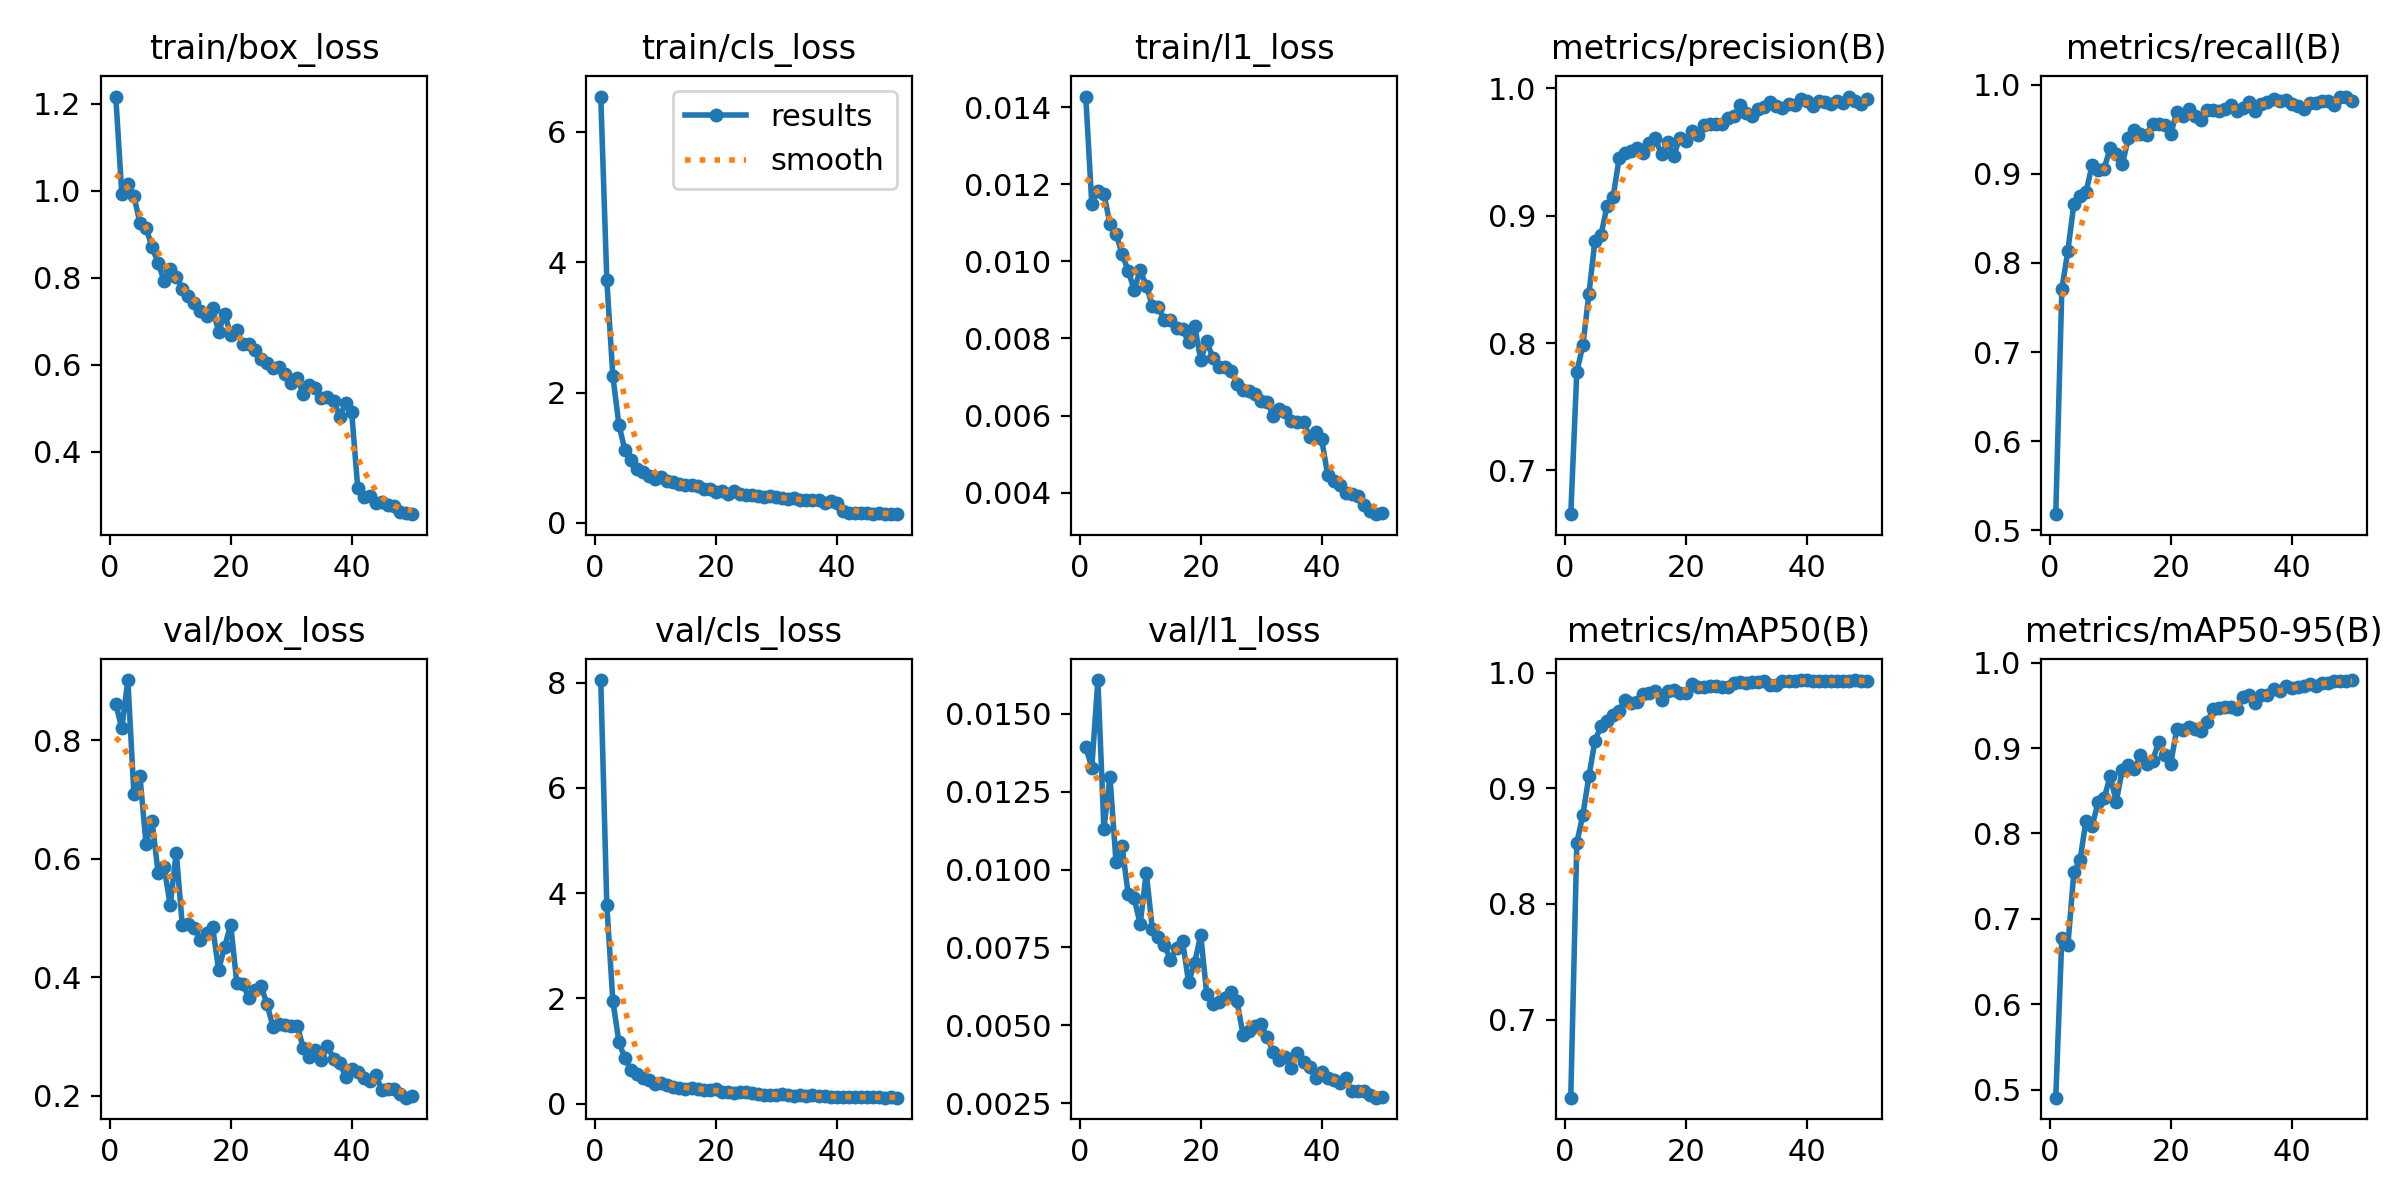
\includegraphics[width=0.8\textwidth]{images/1stage_ablation_results.png}
    \caption{Trainingsmetriken des einstufigen Objektdetektors.}
    \label{fig:ablation_1stage_train}
\end{figure}

\begin{figure}[H]
    \centering
    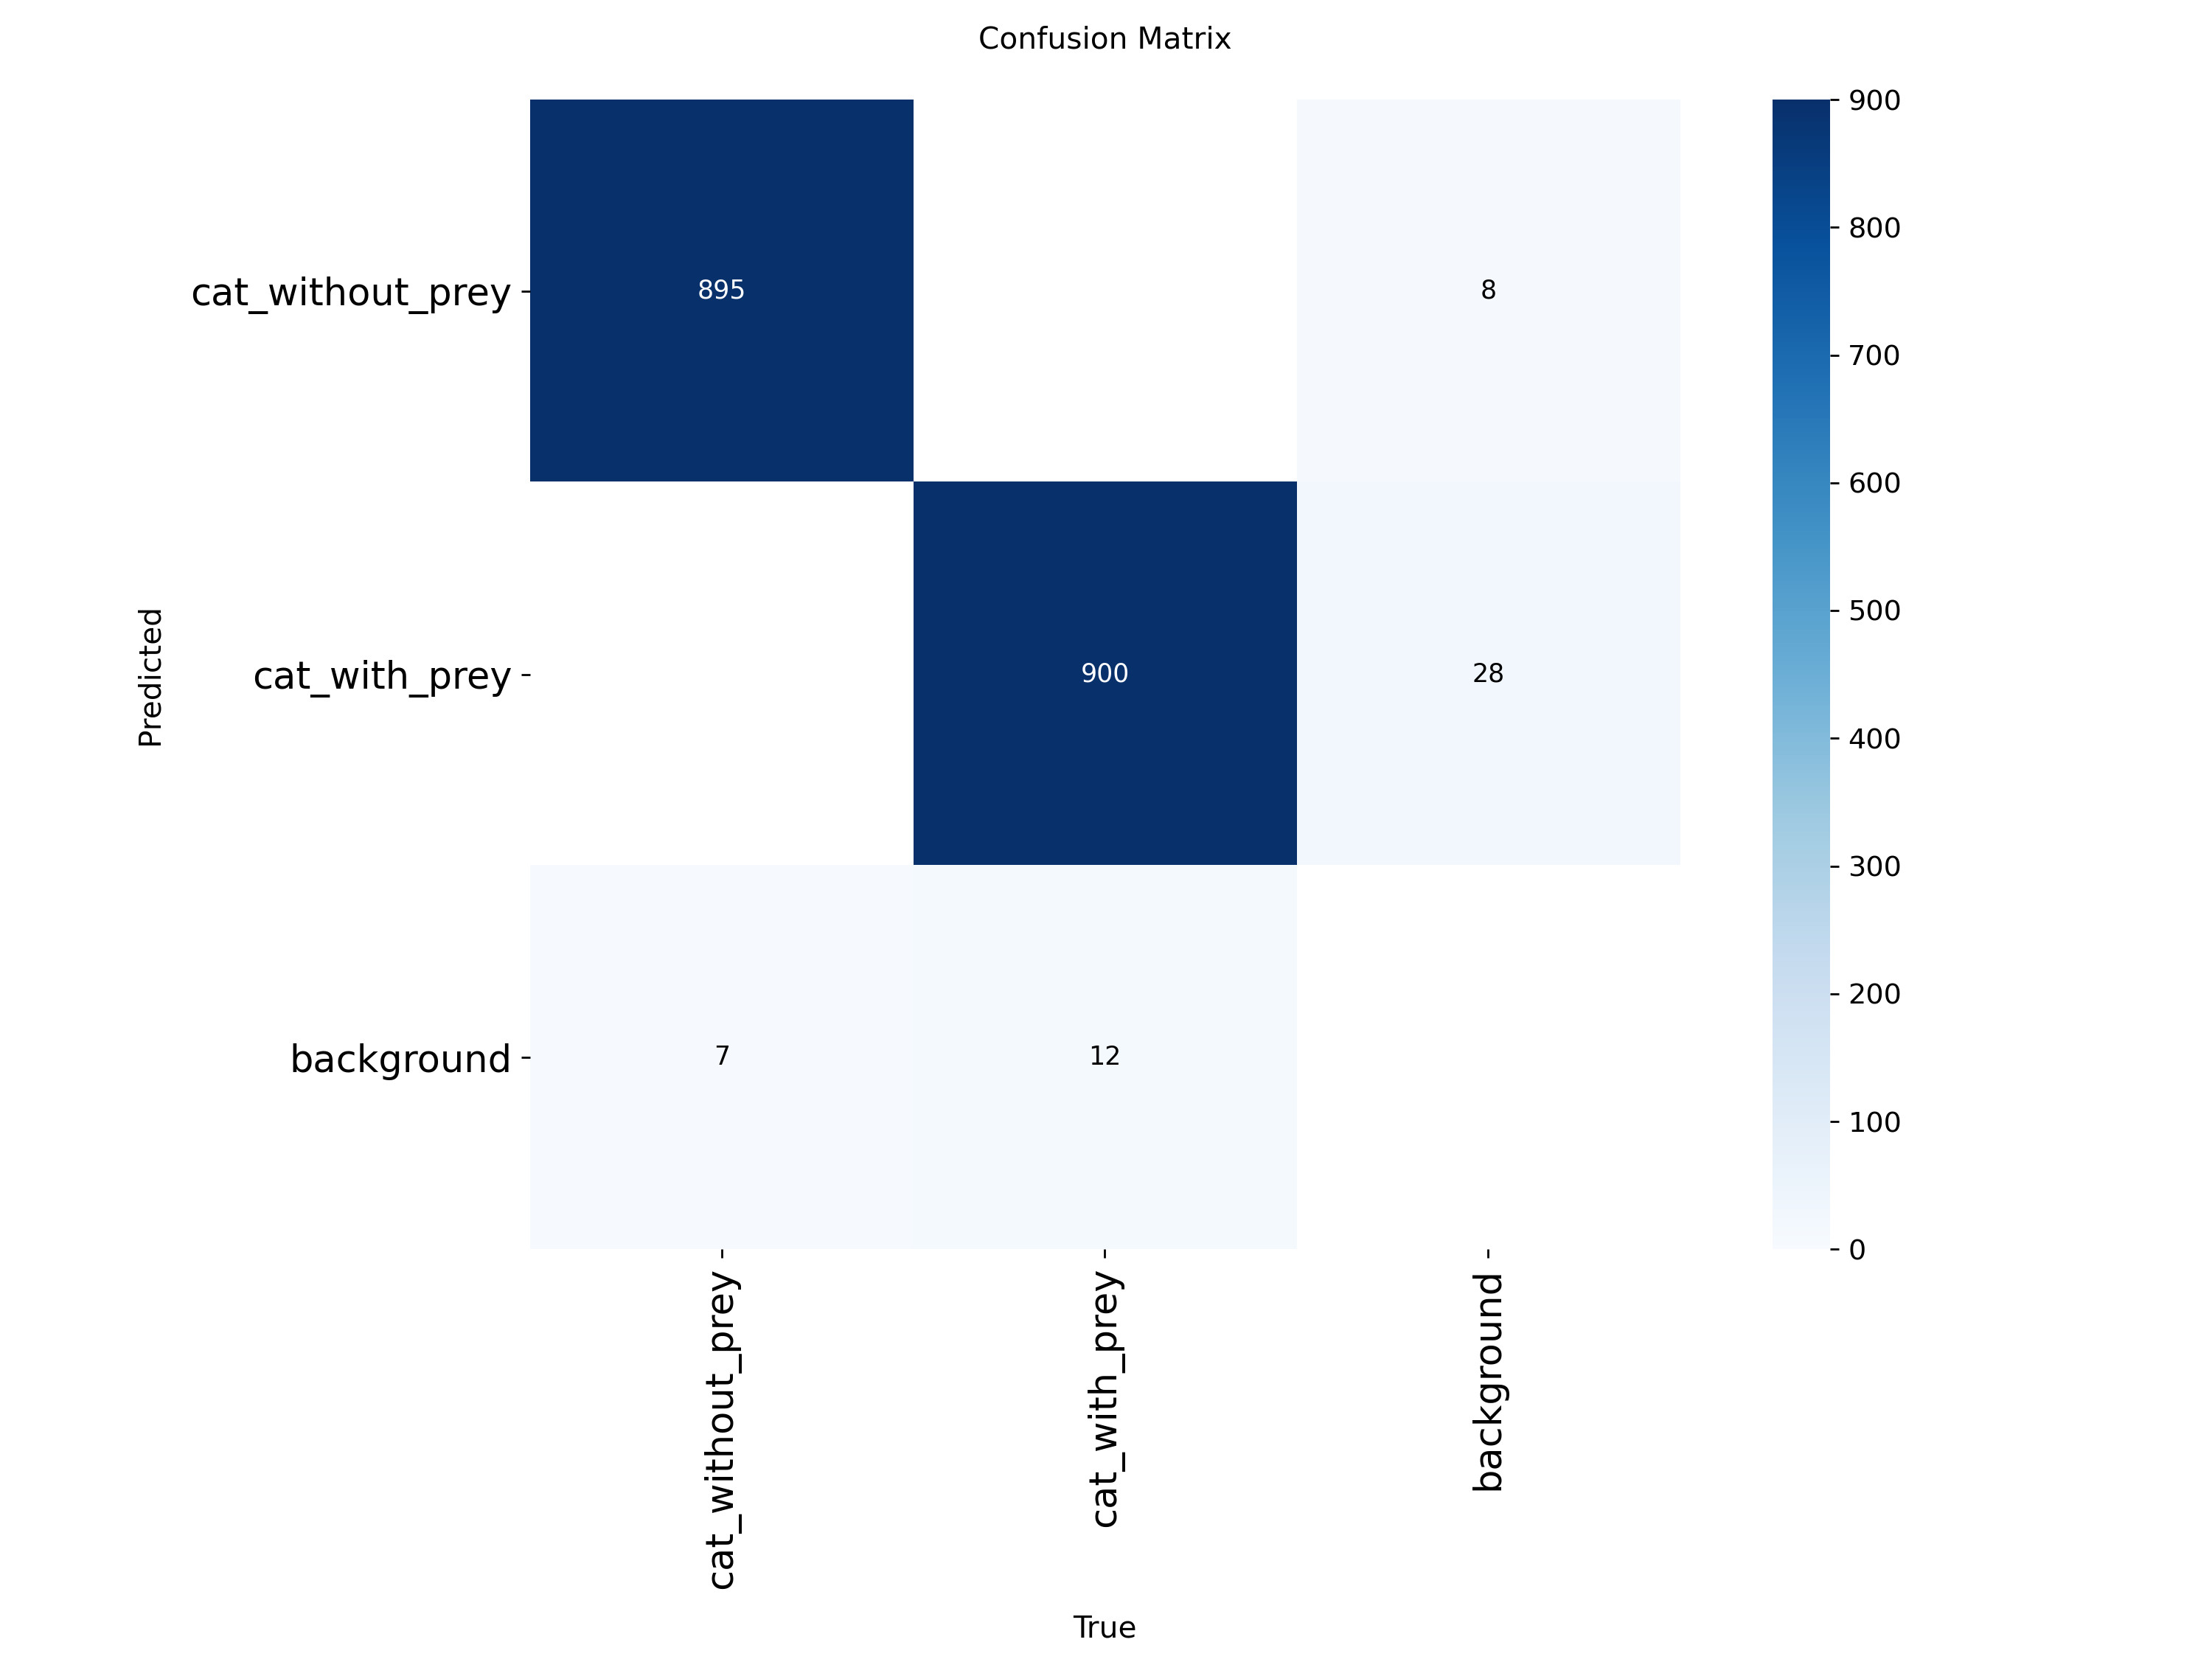
\includegraphics[width=0.7\textwidth]{images/1stage_ablation_confusionmatrix.png}
    \caption{Konfusionsmatrix des einstufigen Objektdetektors auf den Validierungsdaten.}
    \label{fig:ablation_1stage_conf}
\end{figure}


Um die Modelle isoliert zu vergleichen, wurde der Zustandsautomat wieder deaktiviert (\texttt{history\_length=1}). Dabei wurde evaluiert wie viele Sicherheits- und Komfortfehler beide Systeme trafen, sowie wie viele Katzen insgesamt im Video übersehen wurden.
Zusätzlich werden beide Systeme mit dem Zustandsautomaten in der finalen Konfiguration (Zeitfenster von 20 Einzelbildern, Schwellenwert 0,3) ausgewertet. Tabelle~\ref{tab:ablation_1stage} zeigt die Ergebnisse beider Varianten.

\begin{table}[H]
    \centering
    \begin{tabular}{lrrrr}
        \toprule
        & \multicolumn{2}{c}{Ohne Zustandsautomat} & \multicolumn{2}{c}{Mit Zustandsautomat} \\
        \cmidrule(lr){2-3}\cmidrule(lr){4-5}
        Metrik & Zweistufig & Einstufig & Zweistufig & Einstufig \\
        \midrule
        Sicherheitsfehler & 17,3\,\% & 10,1\,\% & 1,6\,\% & 10,6\,\% \\
        Komfortfehler & 20,5\,\% & 62,1\,\% & 4,1\,\% & 30,5\,\% \\
        Präzision & 0,892 & 0,748 & 0,980 & 0,857 \\
        Trefferquote & 0,828 & 0,899 & 0,984 & 0,894 \\
        F1-Maß & 0,859 & 0,817 & 0,982 & 0,875 \\
        Übersehene Katzen & 4,3\,\% & 6,5\,\% & 4,3\,\% & 6,5\,\% \\
        Durchgelassene Beute & 10 von 10 & 10 von 10 & 3 von 10 & 2 von 10 \\
        Entscheidungszeit (sauber) & 0,00\,s & 2,54\,s & 0,67\,s & 3,02\,s \\
        \bottomrule
    \end{tabular}
    \caption{Vergleich des zweistufigen Systems (Detektion und Segmentierung) mit dem einstufigen Objektdetektor, ohne Zustandsautomat (Zeitfenster von einem Einzelbild, Schwellenwert 0,5) und mit Zustandsautomat (Zeitfenster von 20 Einzelbildern, Schwellenwert 0,3).}
    \label{tab:ablation_1stage}
\end{table}

Das einstufige System übersieht mit 6,5\,\% mehr Katzen als der Gesichtsdetektor des zweistufigen Systems (4,3\,\%). Der deutlichste Unterschied zeigt sich beim Komfortfehler: Ohne Zustandsautomat ist die Klappe in 62,1\,\% der Einzelbilder mit sauberen Katzen gesperrt, mit Zustandsautomat in 30,5\,\%. Der einstufige Detektor ordnet saubere Katzen häufig der Klasse \glqq Katze mit Beute\grqq\ zu. Dadurch erreicht er ohne Zustandsautomat zwar einen geringeren Sicherheitsfehler als das zweistufige System, dies geht jedoch zulasten der sauberen Katzen. Mit Zustandsautomat lässt das einstufige System in zwei von zehn Videos Beute durch, das zweistufige System in drei. Der Sicherheitsfehler des einstufigen Systems ist mit 10,6\,\% jedoch mehr als sechsmal so hoch wie jener des zweistufigen Systems (1,6\,\%). Das F1-Maß des zweistufigen Systems liegt mit 0,982 deutlich über jenem des einstufigen Systems (0,875). Zudem benötigt das einstufige System im Mittel 3,02~Sekunden bis zur Freigabe einer sauberen Katze und überschreitet damit die Entscheidungszeit von drei Sekunden.

\subsection{Graustufen gegenüber Farbbildern}
Da die Kamera bei Dunkelheit auf Infrarot-Nachtsicht umschaltet, arbeitet das System durchgehend auf Graustufenbildern. In dieser Studie wird ein auf Graustufenbildern trainiertes System mit einem auf Farbbildern trainierten System verglichen, getrennt nach Tag- und Nachtaufnahmen.
Beide Segmentierungsmodelle besitzen dieselbe Architektur (YOLO26n-seg) und werden mit denselben Trainingsdaten trainiert. Das Farbmodell erhält dabei die ursprünglichen Farbbilder, das Graustufenmodell die in Graustufen umgewandelten Bilder. Der Gesichtsdetektor und der Zustandsautomat (Zeitfenster von 20 Einzelbildern, Schwellenwert 0,3) bleiben in beiden Konfigurationen unverändert. Die Tagaufnahmen umfassen sechs, die Infrarot-Aufnahmen vier Videopaare. Tabelle~\ref{tab:ablation_gray} zeigt die Ergebnisse.

\begin{table}[H]
    \centering
    \small
    \begin{tabular}{lrrrrrr}
        \toprule
        & \multicolumn{2}{c}{Tag} & \multicolumn{2}{c}{Infrarot} & \multicolumn{2}{c}{Gesamt} \\
        \cmidrule(lr){2-3}\cmidrule(lr){4-5}\cmidrule(lr){6-7}
        Metrik & Grau & Farbe & Grau & Farbe & Grau & Farbe \\
        \midrule
        Sicherheitsfehler & 1,9\,\% & 4,4\,\% & 1,2\,\% & 5,6\,\% & 1,6\,\% & 4,9\,\% \\
        Komfortfehler & 6,8\,\% & 1,3\,\% & 0,0\,\% & 0,0\,\% & 4,1\,\% & 0,8\,\% \\
        Präzision & 0,967 & 0,994 & 1,000 & 1,000 & 0,980 & 0,996 \\
        Trefferquote & 0,981 & 0,956 & 0,988 & 0,944 & 0,984 & 0,951 \\
        F1-Maß & 0,974 & 0,975 & 0,994 & 0,971 & 0,982 & 0,973 \\
        Durchgelassene Beute & 2 von 6 & 2 von 6 & 1 von 4 & 2 von 4 & 3 von 10 & 4 von 10 \\
        Entscheidungszeit (Beute) & 0,19\,s & 0,94\,s & 0,03\,s & 0,75\,s & 0,13\,s & 0,86\,s \\
        \bottomrule
    \end{tabular}
    \caption{Vergleich des Segmentierungsmodells für Graustufenbilder mit dem Segmentierungsmodell für Farbbilder, getrennt nach Tag- und Infrarot-Aufnahmen.}
    \label{tab:ablation_gray}
\end{table}

Bei Tagaufnahmen erreichen beide Modelle ein nahezu gleiches F1-Maß (0,974 gegenüber 0,975). Das Graustufenmodell weist einen geringeren Sicherheitsfehler auf (1,9\,\% gegenüber 4,4\,\%), das Farbmodell einen geringeren Komfortfehler (1,3\,\% gegenüber 6,8\,\%). Bei Infrarot-Aufnahmen liegt keine Farbinformation vor. Hier erzielt das Graustufenmodell einen deutlich geringeren Sicherheitsfehler (1,2\,\% gegenüber 5,6\,\%) und ein höheres F1-Maß (0,994 gegenüber 0,971), während beide Modelle keinen Komfortfehler aufweisen. Zudem sperrt das Graustufenmodell die Klappe bei Katzen mit Beute im Mittel nach 0,13~Sekunden, das Farbmodell erst nach 0,86~Sekunden. Über den gesamten Testdatensatz erreicht das Graustufenmodell das höhere F1-Maß und lässt in drei statt vier Videos Beute durch.

\chapter{Diskussion}
\label{sec:diskussion}

Die in Kapitel 6 präsentierten Testergebnisse liefern ein klares Bild der Systemleistung. In diesem Kapitel werden diese Ergebnisse interpretiert und kritisch bewertet. Dabei wird untersucht, inwiefern die Forschungsziele erreicht wurde, wo die grenzen des Systems liegen und welche Funktionalitäten für die Qualität ausschlaggebend waren.

\section{Beantwortung der zentralen Forschungsfrage}
Die primäre Forschungsfrage dieser Arbeit war, ob eine Verarbeitungskette aus Objekterkennung, Bildsegmentierung, Objektverfolgung und zeitlicher Zustandsmodellierung, eine robustere Beute-Erkennung ermöglicht gegenüber Einzelbildmethoden.

Die Evaluierung liefert hierauf eine eindeutig Antwort. Ein einzelbildbasierter Ansatz ist bei der Analyse von Videostreams stark anfällig für Fehler. Bewegungsunschärfe (Motion Blur), wenn die Katze ins Bild läuft, partielle Verdeckungen (Okklusionen) der Beute durch die Pfoten oder rasche Änderungen der Beleuchtung führen zu starken Ungenauigkeiten der Segmentierung. Ohne die zeitliche Aggregation im Zustandsautomaten würde die Zugangskontrolle ständig zwischen den Zuständen \glqq verriegelt\grqq\ und \glqq entriegelt\grqq\ wechseln (Flackern).

Durch die hilfe der \texttt{StateMachine} in Kombination mit ByteTrack wird diese Problem elegant gelöst. Die zeitliche Aggregation über eine Historie von Einzelbildern erzeugt ein robustes Signal, das Ausreißer effektiv glättet. Die Ablationsstudie "Relevanz des Zustandsautomaten" zeigt, dass das System selbst dann richtig entscheidet, wenn einzelne Bilder falsch klassifiziert werden. Somit ist der Beweis erbracht, dass der Zustandsautomat in diesem Anwendungsfall ein wesentlicher Teil ist und zwingend für die Zuverlässigkeit im realen Betrieb ist.

\section{Bewertung des Architektur-Ansatzes}
Die Entscheidung, das Problem in zwei separate neuronale Netze (YOLO-Detektor für das Gesicht und YOLO-Segmentierungsmodell für den Zustand) zu unterteilen, hat sich als äußerst vorteilhaft erwiesen.

\subsection{Stärken der Verarbeitungsketten-Kaskadierung}
Der übliche Ansatz im Bereich maschinelles Sehen bestünde darin, ein einziges Objekterkennungsmodell darauf zu trainieren, direkt die Klassen \glqq Katze\grqq\ und \glqq Beutetier\grqq\ im Gesamtbild zu finden. Bei einer Katzenklappe scheitert dieser Ansatz jedoch häufig. Eine Maus im Maul einer Katze nimmt im Gesamtbild der Kamera nur einen verschwindend geringen Bruchteil der Pixel ein und ist durch das Maul und die Schnurrhaare stark verdeckt. Standard-Objektdetektoren haben immense Schwierigkeiten, derart kleine, okkludierte Objekte zuverlässig mit einem Begrenzungsrahmen zu versehen \cite{tong2020small}.

Der in dieser Arbeit gewählte Kaskadierungs-Ansatz umgeht dieses Problem elegant \cite{baumann2020smartcatflap, zhang2014partbased}. Der erste Detektor muss lediglich das vergleichsweise große und markante Katzengesicht finden – eine triviale Aufgabe für moderne Architekturen wie YOLO26, was sich in der hohen Erkennungsstabilität niederschlug. Durch das anschließende Herausschneiden (Zuschneiden) dieses Bereichs wird die Aufmerksamkeit des nachgelagerten Segmentierungsmodells exklusiv auf die relevante Region fokussiert (Aufmerksamkeitsmechanismus \textit{by design}). Das Segmentierungsmodell muss keine kleine Maus im Hintergrund des Gartens suchen, sondern analysiert lediglich die Pixelstruktur direkt am Maul der Katze.

\subsection{Die Rolle der asymmetrischen Randerweiterung}
Dadurch das die Annotationen des Datensatzes im Detektor (\glqq Cat Dataset\grqq\ von Crawford \cite{kaggle2024cat}) den unteren Teil des Mauls komplett verdecken, ist es unerlässlich für Training und Inferrenz den Begrenzungsrahmen nach untenhin Proportional zu erweitern.

\section{Schwächen, Limitationen und Fehlerquellen}
Aus der Analyse werden die Limitationen des aktuellen Systems genau aufgezeigt. Dadurch entsteht das Potenzial für zukünftige Verbesserungen:

\begin{enumerate}
    \item \textbf{Verlust von Tiefeninformationen:} Dadurch das die Kamera ein 2D Bild aufnimmt kann nicht unterschieden werden, wie weit weg sich ein Objekt unterhalb des Katzenmauls befindet. Daraus folgt, dass das Modell den Unterschied zwischen Hintergrund und Beute nicht zuverlässig trennen kann.
    \item \textbf{Extreme Bewegungsgeschwindigkeit:} Wenn eine Katze fluchtartig durch die Klappe rennt, bleibt sehr wenig Zeit eine klare Aussage zu treffen. Bei einer Laufzeit von ca. 8 FPS verbleiben dem System nur eine Handvoll Einzelbilder zur Analyse.  In diesem Szenario kann die \texttt{StateMachine} ihre Stärke (die zeitliche Glättung) nicht voll ausspielen und die Katze muss warten bis der Zustandsautomat eine klare Entscheidung trifft.
    \item \textbf{Farbe der Katze:} Wenn eine Katze ein sehr dunkles Fell besitzt, hat die Segmentierung Schwierigkeiten und verliert an Genauigkeit. Hier ist es essentiell Daten aus dem Praxisbetrieb zu sammeln, bei denen sich das Modell unsicher war, um genau diese Fälle besser trainieren zu können.
\end{enumerate}

\section{Lokale Datenverarbeitung}
Ziel dieser Arbeit war es auch, dass das System ressourcenschonend konzipiert wird um sicherzustellen dass die Inferrenz auch auf einem Einplatinencomputer lokal operieren kann. Daher viel die Entscheidung auf eine leichtgewichtige Architektur (YOLO26n) und optimierte Formate (TensorFlow Lite). Die dadurch verlorene Genauigkeit wird durch die erreichte Leistung gerechtfertigt (ca. 8 FPS).

Dieser Ansatz beweist, dass eine komplexe Aufgabe auf ressourcenbegrenzter Hardware durch eine intelligent gewählte Architektur gelöst werden kann, ohne dass die Robustheit zu stark beeinträchtigt wird. Dadurch wird eine Auslagerung von Berechnungen in externe Rechenzentren vermieden. Das spart Geld und macht die Lösung zuverlässiger, da keine Internetverbindung notwendig ist.

Abschließend lässt sich sagen, dass die Architektur ihre Aufgabe größtenteils erfüllt. Die verbleibenden Fehlalarme sind kein Architekturfehler, sondern zeigen die Grenzen des begrenzten Segmentierungsdatensatzes auf. Mithilfe des in Kapitel 5 integrierten Modells zum Speichern von Bildern, bei denen das Modell unsicher war, können genau diese Lücken im Datensatz ergänzt werden. So kann das Modell kontinuierlich verbessert werden.
\chapter{Zusammenfassung und Ausblick}
\label{sec:zusammenfassung}

In der vorliegenden Bachelorarbeit wird ein robustes Zugangssystem für Katzen entwickelt, dass das eindringen von Beutetieren (z. B. Mäuse oder Vögel) in den Wohnraum verhindert. Durch die Kombination von mehrschitigen Lernen (eng. Deep Learning) und zeitlicher Aggregation wurde ein System geschaffen, das die einzelbildbasierte Objekterkennung auf den Testdaten deutlich übertrifft.

\section{Zusammenfassung der Erkenntnisse}
\label{subsec:zusammenfassung_erkenntnisse}

Die theoretischen Annahmen konnten durch die praktische Evaluierung erfolgreich validiert werden. In diesem Anwendungsfall ist der klassische monolithische Objektdetektor deutlich ungenauer als die in der Arbeit vorgestellte Verarbeitungskette, die aus einem Objektdetektor, einer Bildsegmentierung und einer zeitlichen Aggregation besteht.

Zunächst detektiert ein YOLO-Detektor das Gesicht der Katze. Um zu verhindern, dass die eventuelle Beute im Maul der Katze okkludiert wird, wird der Ausschnitt des Gesichts um rund eine Gesichtshöhe nach unten erweitert. Im zweiten Schritt analysiert ein YOLO-Segmentierungsmodell, ob sich Beute im Maul der Katze befindet. Um Fehlklassifikationen auszugleichen, muss eine Katze beweisen, dass sie sauber ist. Erst dann darf sie in den Wohnraum eintreten. Dazu wird die Katze über mehrere Sekunden hinweg mithilfe von ByteTrack verfolgt. Der gleitende Durchschnitt der letzten 30 Einzelbilder (was bei 8 Bildern pro Sekunde 3,75 Sekunden entspricht) entscheidet dann, ob die Katze ins Haus darf oder nicht.

Die Evaluierung mit KI-generierten Videodaten zeigte den Erfolg des gewählten Architektur-Ansatzes. Das System gab die Klappe in keinem Einzelbild mit Beute fälschlicherweise frei und sperrte keine saubere Katze aus. Der gewählte Schwellenwert von 0,3 sperrt die Klappe bereits bei geringen Anzeichen von Beute. Saubere Katzen warten dafür im Mittel 2,0 Sekunden, bis die Klappe freigegeben wird. Das System erweist sich somit als sehr praxistauglich und läuft mit durchschnittlich 8 Bildern pro Sekunde ressourcenschonend auf lokalen Endgeräten.

Somit konnte die zentrale Forschungsfrage bejaht werden. Eine Kombination aus Objekterkennung, Objektverfolgung und zeitlicher Glättung ist deutlich robuster als herkömmliche Einzelbildauswertungen.

\section{Ausblick und Weiterentwicklungsmöglichkeiten}
\label{subsec:ausblick}

Obwohl das System in seiner aktuellen Form bereits zuverlässig Beutetiere aussperrt, zeigt die Praxis, dass auch dieser Ansatz Schwächen und Limitierungen hat. Das eröffnet die Möglichkeit, konkrete Ansatzpunkte für zukünftige Verbesserungen zu identifizieren.

\subsection{Kontinuierliches Sammeln unsicherer Beispiele}
Die vielversprechendste Methode, um die Systemleistung zu steigern, ist die Erweiterung des Datensatzes für Katzen mit Beute. Um dieses Ziel zu automatisieren, verfügt die Applikation über eine Funktionalität, die Bilder speichert, bei denen die Bildsegmentierung unsicher war. Dadurch können zukünftige Arbeiten diesen stetig wachsenden Datensatz nutzen, um das YOLO-Segmentierungsmodell iterativ nachzutrainieren. Sobald das Segmentierungsmodell aus diesen Fehlern lernen kann, kann die Fehlalarmrate des gesamten Systems sinken. Dieses Vorgehen entspricht dem Prinzip des aktiven Lernens, bei dem gezielt jene Beispiele ausgewählt werden, bei denen das Modell am unsichersten ist \cite{settles2009active}.

\subsection{Verlust der Tiefeninformationen}
Eine weitere Einschränkung ist der Verlust von 3D-Informationen im Bild. Dadurch kann es passieren, dass Objekte im Hintergrund oder sogar der Körper der Katze fälschlicherweise als \glqq im Maul der Katze\grqq\ interpretiert werden. Eine mögliche Erweiterung bestünde darin, diese 3D-Informationen mithilfe von Stereo-Kameras oder Time-of-Flight-Sensoren zurückzugewinnen. Dadurch könnten Fehlalarme herausgefiltert werden, bei denen sich das vermeintliche Beutetier weit hinter dem Maul der Katze befindet.

\subsection{Hardware-Beschleunigung}
Derzeit wird das System ausschließlich auf der CPU ausgeführt. Ein Wechsel auf eine dedizierte Hardware (z. B. Google Coral) würde die Anzahl der pro Sekunde verarbeiteten Bilder deutlich erhöhen. Dadurch können wir in der gleichen Zeit mehr Daten der Katze sammeln, was die zeitliche Glättung verbessern würde. Das Flackern des Systems würde dadurch noch weiter eingeschränkt.

\vspace{0.5cm}

Abschließend lässt sich zusammenfassen, dass die in dieser Arbeit entwickelte Verarbeitungskette ein kompaktes und robustes Fundament bildet. Sie löst das Problem des unerwünschten Beuteeintrags durch Katzen zuverlässig und ermöglicht zugleich spannende Erweiterungen und Verbesserungen.


\backmatter

\MakeBibliography

\end{document}
